% =============================================================================
% NeurIPS 2026 Paper: TinkerRL Lab
% =============================================================================
% Template: NeurIPS 2026 (based on neurips_2025.sty)
% Track: Evaluations & Datasets (recommended) or Main Track
% =============================================================================
% SUBMISSION NOTE: For anonymous submission, comment out author block above
% and uncomment: \author{Anonymous Authors}
% Also anonymize: GitHub URLs, HuggingFace URLs, PES University references
% Replace with: \url{https://anonymous.4open.science/r/tinker-rl-lab}

\documentclass{article}

% NeurIPS 2026 style (download from https://neurips.cc)
% \usepackage{neurips_2025}       % For camera-ready
\usepackage[preprint,nonatbib]{neurips_2026} % For preprint (remove for submission)
\usepackage[numbers]{natbib}
% \usepackage[nonatbib]{neurips_2026} % Submission mode (anonymized, line numbers)

\usepackage[utf8]{inputenc}
\usepackage[T1]{fontenc}
\usepackage{hyperref}
\usepackage{url}
\usepackage{booktabs}
\usepackage{amsfonts}
\usepackage{amsmath}
\usepackage{amssymb}
\usepackage{nicefrac}
\usepackage{microtype}
\usepackage{xcolor}
\usepackage{graphicx}
\usepackage{subcaption}
\usepackage{algorithm}
\usepackage{algorithmic}
\usepackage{multirow}
\usepackage{enumitem}
\usepackage{tikz}
\usetikzlibrary{positioning, fit, arrows.meta, backgrounds, calc, shadows, shapes.geometric, shapes.misc, decorations.pathreplacing}

% Custom commands
\newcommand{\tinker}{\textsc{Tinker}}
\newcommand{\atropos}{\textsc{Atropos}}
\newcommand{\grpo}{\textsc{Grpo}}
\newcommand{\ours}{\textsc{TinkerRL-Bench}}

\title{A Unified Benchmark for RL Post-Training of Language Models}

% For submission, use anonymous authors:
% \author{Anonymous Authors}

\author{
  Arvind C R\thanks{Equal contribution.} \\
  PES University\\
  \texttt{arvindcr4@gmail.com} \\
  \And
  Sandhya Jeyaraj\footnotemark[1] \\
  PES University\\
  \texttt{sandhya.jeyaraj2014@gmail.com} \\
  \And
  Madhu Kumara L \\
  PES University\\
  \texttt{madhukumara1993@gmail.com} \\
  \And
  Mohammad Rafi \\
  PES University\\
  \texttt{gmd.rafi.2024@gmail.com} \\
  \And
  Dhruva N Murthy \\
  PES University\\
  \texttt{dhruva.n.murthy@gmail.com} \\
  \And
  Arumugam K \\
  PES University\\
  \texttt{chettyarumugam@mail.com} \\
  \And
  Anwesh Reddy Paduri \\
  Great Learning / PES University\\
  \texttt{anwesh@greatlearning.in} \\
  \And
  Narayana Darapaneni \\
  Northwestern University / Great Learning\\
  \texttt{narayana.darapaneni@northwestern.edu} \\
}

% Custom command for partial answers in NeurIPS checklist
\newcommand{\answerPartial}[1][]{\textcolor{purple}{[Partial] #1}}

\begin{document}
\sloppy
\hbadness=10000
\vbadness=10000
\hfuzz=2pt

\maketitle

% =============================================================================
% Abstract reframed around F1--F5 (see sections/abstract.tex)
% =============================================================================
% Abstract — reframed around the five empirical discoveries (F1--F5)
% Drop-in include: % =============================================================================
% Abstract — reframed around the five empirical discoveries (F1--F5)
% Drop-in include: % =============================================================================
% Abstract — reframed around the five empirical discoveries (F1--F5)
% Drop-in include: \input{sections/abstract}
% Target: <= 250 words
% =============================================================================
\begin{abstract}
RL post-training of language models is now shaped by a handful of algorithms
(PPO, GRPO, DPO) and a growing fleet of frameworks (TRL, \tinker{}, OpenRLHF,
veRL), yet which choices actually drive performance remains empirically
unsettled.  We present \ours{}, a controlled study of 79 runs spanning 7 RL
libraries, 5 model families, and 0.6B--$\sim$1T parameters, designed to isolate
cause from confound on GSM8K, MATH-500, HumanEval, and tool-use.

Five discoveries reframe what should be measured and reported.
\textbf{(F1) ZVF dominance.}  Zero-Variance Fraction---the share of GRPO
groups with no within-group reward variance---is the single strongest predictor
of final reward (Pearson $r{=}{-}0.769$, $p{=}0.0008$), outranking scale,
algorithm, and library, and elevates 5--10 steps before reward collapses.
\textbf{(F2) Inverted-U in group size.}  $G{=}32$ maximizes gradient
utilization (54.5\%) and latest saturation onset (step 29); smaller and larger
$G$ are both worse, contradicting ``more rollouts is better.''
\textbf{(F3) Base vs.\ instruct dichotomy.}  Instruction tuning delivers a
$+0.922$ GSM8K delta (0.047$\to$0.969); Qwen3-30B-A3B-Instruct hits 100\%
last-10 where its base twin stalls at 32.5\%.  SFT, not RL, is the
trainability gate.
\textbf{(F4) PPO vs.\ GRPO is model-dependent.}  GRPO beats PPO on Qwen3-8B
(34.4\% vs.\ 22.5\%); PPO beats GRPO on Llama-3.1-8B (97.5\% vs.\ 84.4\%,
Mann-Whitney $r{=}0.94$, $p{<}10^{-10}$)---the ranking reverses across
families.
\textbf{(F5) Kimi-K2 sustained ceiling.}  Where Nemotron-120B peaks 87.5\%
then collapses to 16.2\%, Kimi-K2 holds peak 100\% / last-10 80\% in 20 steps
(Kimi-K2-Thinking: 91.7\% last-10)---ceiling stability is architecture-
and pre-training-conditional, not a monotone function of scale.

Code, 79 run logs, and checkpoints:
\url{https://github.com/arvindcr4/tinker-rl-lab}.
\end{abstract}

% Target: <= 250 words
% =============================================================================
\begin{abstract}
RL post-training of language models is now shaped by a handful of algorithms
(PPO, GRPO, DPO) and a growing fleet of frameworks (TRL, \tinker{}, OpenRLHF,
veRL), yet which choices actually drive performance remains empirically
unsettled.  We present \ours{}, a controlled study of 79 runs spanning 7 RL
libraries, 5 model families, and 0.6B--$\sim$1T parameters, designed to isolate
cause from confound on GSM8K, MATH-500, HumanEval, and tool-use.

Five discoveries reframe what should be measured and reported.
\textbf{(F1) ZVF dominance.}  Zero-Variance Fraction---the share of GRPO
groups with no within-group reward variance---is the single strongest predictor
of final reward (Pearson $r{=}{-}0.769$, $p{=}0.0008$), outranking scale,
algorithm, and library, and elevates 5--10 steps before reward collapses.
\textbf{(F2) Inverted-U in group size.}  $G{=}32$ maximizes gradient
utilization (54.5\%) and latest saturation onset (step 29); smaller and larger
$G$ are both worse, contradicting ``more rollouts is better.''
\textbf{(F3) Base vs.\ instruct dichotomy.}  Instruction tuning delivers a
$+0.922$ GSM8K delta (0.047$\to$0.969); Qwen3-30B-A3B-Instruct hits 100\%
last-10 where its base twin stalls at 32.5\%.  SFT, not RL, is the
trainability gate.
\textbf{(F4) PPO vs.\ GRPO is model-dependent.}  GRPO beats PPO on Qwen3-8B
(34.4\% vs.\ 22.5\%); PPO beats GRPO on Llama-3.1-8B (97.5\% vs.\ 84.4\%,
Mann-Whitney $r{=}0.94$, $p{<}10^{-10}$)---the ranking reverses across
families.
\textbf{(F5) Kimi-K2 sustained ceiling.}  Where Nemotron-120B peaks 87.5\%
then collapses to 16.2\%, Kimi-K2 holds peak 100\% / last-10 80\% in 20 steps
(Kimi-K2-Thinking: 91.7\% last-10)---ceiling stability is architecture-
and pre-training-conditional, not a monotone function of scale.

Code, 79 run logs, and checkpoints:
\url{https://github.com/arvindcr4/tinker-rl-lab}.
\end{abstract}

% Target: <= 250 words
% =============================================================================
\begin{abstract}
RL post-training of language models is now shaped by a handful of algorithms
(PPO, GRPO, DPO) and a growing fleet of frameworks (TRL, \tinker{}, OpenRLHF,
veRL), yet which choices actually drive performance remains empirically
unsettled.  We present \ours{}, a controlled study of 79 runs spanning 7 RL
libraries, 5 model families, and 0.6B--$\sim$1T parameters, designed to isolate
cause from confound on GSM8K, MATH-500, HumanEval, and tool-use.

Five discoveries reframe what should be measured and reported.
\textbf{(F1) ZVF dominance.}  Zero-Variance Fraction---the share of GRPO
groups with no within-group reward variance---is the single strongest predictor
of final reward (Pearson $r{=}{-}0.769$, $p{=}0.0008$), outranking scale,
algorithm, and library, and elevates 5--10 steps before reward collapses.
\textbf{(F2) Inverted-U in group size.}  $G{=}32$ maximizes gradient
utilization (54.5\%) and latest saturation onset (step 29); smaller and larger
$G$ are both worse, contradicting ``more rollouts is better.''
\textbf{(F3) Base vs.\ instruct dichotomy.}  Instruction tuning delivers a
$+0.922$ GSM8K delta (0.047$\to$0.969); Qwen3-30B-A3B-Instruct hits 100\%
last-10 where its base twin stalls at 32.5\%.  SFT, not RL, is the
trainability gate.
\textbf{(F4) PPO vs.\ GRPO is model-dependent.}  GRPO beats PPO on Qwen3-8B
(34.4\% vs.\ 22.5\%); PPO beats GRPO on Llama-3.1-8B (97.5\% vs.\ 84.4\%,
Mann-Whitney $r{=}0.94$, $p{<}10^{-10}$)---the ranking reverses across
families.
\textbf{(F5) Kimi-K2 sustained ceiling.}  Where Nemotron-120B peaks 87.5\%
then collapses to 16.2\%, Kimi-K2 holds peak 100\% / last-10 80\% in 20 steps
(Kimi-K2-Thinking: 91.7\% last-10)---ceiling stability is architecture-
and pre-training-conditional, not a monotone function of scale.

Code, 79 run logs, and checkpoints:
\url{https://github.com/arvindcr4/tinker-rl-lab}.
\end{abstract}


% Introduction reframed around F1--F5 (see sections/intro.tex)
% =============================================================================
% Introduction — conservative, evidence-aligned framing
% Drop-in include: % =============================================================================
% Introduction — conservative, evidence-aligned framing
% Drop-in include: % =============================================================================
% Introduction — conservative, evidence-aligned framing
% Drop-in include: \input{sections/intro}
% Target: <= 1.5 pages
% =============================================================================
\section{Introduction}
\label{sec:intro}

Reinforcement learning post-training now underpins much of modern
language-model reasoning and alignment~\citep{ouyang2022training,%
guo2025deepseekr1nature}, but empirical claims in this area are often hard to
compare. PPO~\citep{schulman2017proximal}, GRPO~\citep{shao2024deepseekmath},
and DPO~\citep{rafailov2024direct} are usually evaluated on different model
families, with different framework defaults, different reward functions, and
different notions of ``success.'' What the field needs is not another
leaderboard but a substrate that separates algorithmic conclusions from
implementation, initialization, and task-design effects.

\ours{} is an attempt at such a substrate. It aggregates 79 runs spanning 7 RL
libraries, 5 model families, 32+ checkpoints, and scales from 0.6B to
$\sim$1T parameters, with common reporting conventions and released artifacts.
At the same time, we emphasize a central caveat: the current benchmark is
\emph{not} uniformly mature across tasks. The strongest evidence comes from
short-horizon GSM8K experiments with verifiable binary rewards. Frontier API
runs, tool-use experiments, and code-generation studies are useful case
studies, but many remain single-seed, short-horizon, partially completed, or
custom-evaluated.

The first contribution of the benchmark is therefore methodological rather than
triumphalist: it makes visible how much end-to-end stack choice matters. In our
results, model family, initialization, rollout regime, and framework defaults
can all change the apparent algorithm ranking. Several comparisons that look
like ``PPO vs.\ GRPO'' are better understood as \emph{stack-level comparisons},
because the training backends differ in tokenizer/runtime integration, managed
defaults, and rollout plumbing. This is precisely why a shared measurement
substrate is needed.

Our second contribution is a descriptive diagnostic for sparse-reward GRPO:
Zero-Variance Fraction (ZVF), the fraction of rollout groups with identical
rewards, together with Gradient Utilization (GU = $1-\mathrm{ZVF}$). ZVF is
useful because it directly reveals when within-group contrast disappears.
However, because our main tasks use binary outcome rewards, ZVF is mechanically
coupled to reward sparsity, group size, and baseline accuracy. We therefore use
ZVF/GU as diagnostics of signal degeneracy, not as proof of an independent or
causal failure mode beyond simpler observables such as reward mean, entropy,
advantage variance, or divergence proxies.

Our third contribution is a set of targeted ablations on trainability. In the
current benchmark, instruction-tuned checkpoints are consistently easier to
optimize than comparable base models, and intermediate rollout group sizes
outperform extremes in limited sweeps. These observations support a cautious
claim: whether RL fine-tuning works at all often depends more on
initialization and reward-bearing rollout structure than on the nominal choice
of RL algorithm. They do \emph{not} yet justify a universal optimal group size
or a general ``SFT dominates RL'' law.

Finally, we explicitly separate training reward from held-out generalization.
For Qwen3-8B on GSM8K, a five-seed held-out evaluation yields 83.3\% accuracy,
but the base model under the same greedy protocol already scores 82.0\%; the
+1.3 percentage-point delta is not statistically significant ($p{=}0.26$).
This negative control matters: strong online reward curves do not by themselves
establish generalization gains. We release the benchmark, step-level traces,
and checkpoints so that stronger follow-up work can test exactly these failure
points.

% Target: <= 1.5 pages
% =============================================================================
\section{Introduction}
\label{sec:intro}

Reinforcement learning post-training now underpins much of modern
language-model reasoning and alignment~\citep{ouyang2022training,%
guo2025deepseekr1nature}, but empirical claims in this area are often hard to
compare. PPO~\citep{schulman2017proximal}, GRPO~\citep{shao2024deepseekmath},
and DPO~\citep{rafailov2024direct} are usually evaluated on different model
families, with different framework defaults, different reward functions, and
different notions of ``success.'' What the field needs is not another
leaderboard but a substrate that separates algorithmic conclusions from
implementation, initialization, and task-design effects.

\ours{} is an attempt at such a substrate. It aggregates 79 runs spanning 7 RL
libraries, 5 model families, 32+ checkpoints, and scales from 0.6B to
$\sim$1T parameters, with common reporting conventions and released artifacts.
At the same time, we emphasize a central caveat: the current benchmark is
\emph{not} uniformly mature across tasks. The strongest evidence comes from
short-horizon GSM8K experiments with verifiable binary rewards. Frontier API
runs, tool-use experiments, and code-generation studies are useful case
studies, but many remain single-seed, short-horizon, partially completed, or
custom-evaluated.

The first contribution of the benchmark is therefore methodological rather than
triumphalist: it makes visible how much end-to-end stack choice matters. In our
results, model family, initialization, rollout regime, and framework defaults
can all change the apparent algorithm ranking. Several comparisons that look
like ``PPO vs.\ GRPO'' are better understood as \emph{stack-level comparisons},
because the training backends differ in tokenizer/runtime integration, managed
defaults, and rollout plumbing. This is precisely why a shared measurement
substrate is needed.

Our second contribution is a descriptive diagnostic for sparse-reward GRPO:
Zero-Variance Fraction (ZVF), the fraction of rollout groups with identical
rewards, together with Gradient Utilization (GU = $1-\mathrm{ZVF}$). ZVF is
useful because it directly reveals when within-group contrast disappears.
However, because our main tasks use binary outcome rewards, ZVF is mechanically
coupled to reward sparsity, group size, and baseline accuracy. We therefore use
ZVF/GU as diagnostics of signal degeneracy, not as proof of an independent or
causal failure mode beyond simpler observables such as reward mean, entropy,
advantage variance, or divergence proxies.

Our third contribution is a set of targeted ablations on trainability. In the
current benchmark, instruction-tuned checkpoints are consistently easier to
optimize than comparable base models, and intermediate rollout group sizes
outperform extremes in limited sweeps. These observations support a cautious
claim: whether RL fine-tuning works at all often depends more on
initialization and reward-bearing rollout structure than on the nominal choice
of RL algorithm. They do \emph{not} yet justify a universal optimal group size
or a general ``SFT dominates RL'' law.

Finally, we explicitly separate training reward from held-out generalization.
For Qwen3-8B on GSM8K, a five-seed held-out evaluation yields 83.3\% accuracy,
but the base model under the same greedy protocol already scores 82.0\%; the
+1.3 percentage-point delta is not statistically significant ($p{=}0.26$).
This negative control matters: strong online reward curves do not by themselves
establish generalization gains. We release the benchmark, step-level traces,
and checkpoints so that stronger follow-up work can test exactly these failure
points.

% Target: <= 1.5 pages
% =============================================================================
\section{Introduction}
\label{sec:intro}

Reinforcement learning post-training now underpins much of modern
language-model reasoning and alignment~\citep{ouyang2022training,%
guo2025deepseekr1nature}, but empirical claims in this area are often hard to
compare. PPO~\citep{schulman2017proximal}, GRPO~\citep{shao2024deepseekmath},
and DPO~\citep{rafailov2024direct} are usually evaluated on different model
families, with different framework defaults, different reward functions, and
different notions of ``success.'' What the field needs is not another
leaderboard but a substrate that separates algorithmic conclusions from
implementation, initialization, and task-design effects.

\ours{} is an attempt at such a substrate. It aggregates 79 runs spanning 7 RL
libraries, 5 model families, 32+ checkpoints, and scales from 0.6B to
$\sim$1T parameters, with common reporting conventions and released artifacts.
At the same time, we emphasize a central caveat: the current benchmark is
\emph{not} uniformly mature across tasks. The strongest evidence comes from
short-horizon GSM8K experiments with verifiable binary rewards. Frontier API
runs, tool-use experiments, and code-generation studies are useful case
studies, but many remain single-seed, short-horizon, partially completed, or
custom-evaluated.

The first contribution of the benchmark is therefore methodological rather than
triumphalist: it makes visible how much end-to-end stack choice matters. In our
results, model family, initialization, rollout regime, and framework defaults
can all change the apparent algorithm ranking. Several comparisons that look
like ``PPO vs.\ GRPO'' are better understood as \emph{stack-level comparisons},
because the training backends differ in tokenizer/runtime integration, managed
defaults, and rollout plumbing. This is precisely why a shared measurement
substrate is needed.

Our second contribution is a descriptive diagnostic for sparse-reward GRPO:
Zero-Variance Fraction (ZVF), the fraction of rollout groups with identical
rewards, together with Gradient Utilization (GU = $1-\mathrm{ZVF}$). ZVF is
useful because it directly reveals when within-group contrast disappears.
However, because our main tasks use binary outcome rewards, ZVF is mechanically
coupled to reward sparsity, group size, and baseline accuracy. We therefore use
ZVF/GU as diagnostics of signal degeneracy, not as proof of an independent or
causal failure mode beyond simpler observables such as reward mean, entropy,
advantage variance, or divergence proxies.

Our third contribution is a set of targeted ablations on trainability. In the
current benchmark, instruction-tuned checkpoints are consistently easier to
optimize than comparable base models, and intermediate rollout group sizes
outperform extremes in limited sweeps. These observations support a cautious
claim: whether RL fine-tuning works at all often depends more on
initialization and reward-bearing rollout structure than on the nominal choice
of RL algorithm. They do \emph{not} yet justify a universal optimal group size
or a general ``SFT dominates RL'' law.

Finally, we explicitly separate training reward from held-out generalization.
For Qwen3-8B on GSM8K, a five-seed held-out evaluation yields 83.3\% accuracy,
but the base model under the same greedy protocol already scores 82.0\%; the
+1.3 percentage-point delta is not statistically significant ($p{=}0.26$).
This negative control matters: strong online reward curves do not by themselves
establish generalization gains. We release the benchmark, step-level traces,
and checkpoints so that stronger follow-up work can test exactly these failure
points.


% =============================================================================
% Related Work (v2)
% =============================================================================
% Related Work v2 --- expanded related work for NeurIPS 2026 submission
% Replaces the Related Work section in paper/main.tex (sec:related).
% Grouped into five themes:
%   (1) RL algorithms for LLMs
%   (2) Reasoning RL (and process reward models)
%   (3) Tool-use RL
%   (4) Scaling laws for RL post-training
%   (5) Frameworks, benchmarks, and reproducibility
% Every paragraph references entries defined in paper/references.bib.
% =============================================================================

\section{Related Work}
\label{sec:related}

\ours{} sits at the intersection of five rapidly evolving lines of work:
policy-gradient \emph{algorithms} for language models, RL for \emph{reasoning}
(including process reward models), RL for \emph{tool use} and agentic behaviour,
empirical \emph{scaling laws} for RL post-training, and the \emph{frameworks}
and \emph{benchmarks} that instantiate these algorithms. We situate our
contribution against more than fifty recent works; entries marked with
\textsuperscript{\dag} appeared at NeurIPS, ICML, or ICLR in the 2025--2026 cycle.

% -----------------------------------------------------------------------------
\subsection{RL Algorithms for Large Language Models}
\label{sec:related:algos}

Proximal Policy Optimization (PPO)~\cite{schulman2017proximal} is the workhorse
algorithm behind InstructGPT-style RLHF~\cite{ouyang2022training,
christiano2017deeprlhf, stiennon2020summarize, bai2022hhrlhf, bai2022claudecai}
and has dominated production deployments for five years. Direct Preference
Optimization~\cite{rafailov2024direct} reframed preference learning as
contrastive classification and spawned a large family of RL-free alternatives,
including IPO~\cite{azar2024ipo}, KTO~\cite{ethayarajh2024kto},
SimPO~\cite{meng2024simpo}, ORPO~\cite{hong2024orpo}, and
SLiC~\cite{zhao2023slic}, all of which we consider as no-rollout baselines in
our cross-library protocol.

The current wave is defined by \emph{group-relative} policy gradient methods.
GRPO was introduced with DeepSeekMath~\cite{shao2024deepseekmath} and
popularised by DeepSeek-R1~\cite{guo2025deepseekr1,guo2025deepseekr1nature}, the
first reasoning RL method published in \emph{Nature}, which showed that
pure outcome-reward RL can elicit chain-of-thought behaviour from a base
model without supervised cold-start data. A second wave of refinements
dissects the biases of vanilla GRPO. Dr.~GRPO~\cite{liu2025drgrpo} removes a
response-length bias and a question-difficulty amplification bias by using a
constant loss normaliser and dropping the standard-deviation denominator in the
advantage. GDPO~\cite{liu2026gdpo} decouples group-relative normalisation per
reward component, preventing advantage collapse when rewards are multi-valued.
MAD~GRPO~\cite{wang2025madgrpo} replaces the standard-deviation advantage
scaler with the Median Absolute Deviation for heavy-tailed reward
distributions. G$^{2}$RPO~\cite{hu2026openvlthinker} forces per-prompt
advantages to match $\mathcal{N}(0,1)$ to fix reward-topology variance in
multimodal settings. Wu et al.~\cite{wu2025grpo_dpo} prove that GRPO is
``secretly DPO'' --- the group-level advantage is an implicit contrastive
objective --- and show that 2-GRPO retains $98.1\%$ of the performance of
16-GRPO at $12.5\%$ of the rollout budget. iGRPO~\cite{hatamizadeh2026igrpo}
adds a two-stage self-feedback loop that conditions subsequent rollouts on the
policy's best draft, reaching $85.6\%$ on AIME24. AERO~\cite{zhang2026aero}
combines adaptive rollout sizing, rejection sampling, and a Bayesian posterior
over prompt difficulty to eliminate zero-advantage dead zones, cutting RL
compute by $48\%$. Target Policy Optimization (TPO)~\cite{kaddour2026tpo}
decouples target-distribution construction from policy fitting: given scored
completions, TPO builds a target $q \propto p_{\text{old}} \exp(u)$ and fits
the policy via cross-entropy, giving a zero-gradient fixed point once the
policy matches the target. RGRA~\cite{carrino2026rgra} shows that PPO-style
clipping is unnecessary on top of group relative advantages, outperforming
GRPO on 17 of 27 comparisons. EFRame~\cite{wang2025eframe} augments GRPO with
exploration rollouts and experience replay for rare trajectories.

A parallel thread focuses on \emph{production-scale} refinements. GSPO, from
the Qwen team~\cite{qwen2025gspo}, redefines the importance ratio at the
sequence level (rather than token level) and was credited with stabilising the
Qwen3 series, especially its Mixture-of-Experts variants. DAPO, from
ByteDance~\cite{yu2025dapo}, contributes asymmetric Clip-Higher, dynamic
sampling, token-level loss normalisation, and overlong filtering, reaching
$50$ points on AIME~2024 with a 32B model. Kimi-K1.5~\cite{team2025kimi15,
team2025kimik2} and DeepSeek-V3~\cite{deepseek2024v3} both report their own
GRPO variants and online mirror-descent-style updates. Orthogonal
production variants include
Flow-GRPO~\cite{liu2025flowgrpo}, VAPO~\cite{bytedance2025vapo}, and
Dr.~SAC~\cite{ahmadian2024backtobasics}; the last argues that classical
REINFORCE with a value baseline, when carefully implemented, matches GRPO on
several RLHF tasks.

A third thread attacks the \emph{zero-variance failure mode} (ZVF) directly.
AERO~\cite{zhang2026aero} and GRESO~\cite{zhang2026greso} pre-screen prompts
before sampling; CPPO~\cite{lin2025cppo} prunes completions post-rollout,
giving up to $7.98\times$ speedup on GSM8K. NGRPO~\cite{nan2025ngrpo} adds
Advantage Calibration and asymmetric clipping so that all-incorrect groups
still carry gradient. Scaf-GRPO~\cite{zhang2025scaffgrpo} injects tiered
scaffolding hints when learning stagnates, boosting AIME~2024 by $44.3\%$
relative. EBPO~\cite{han2026ebpo} uses a Bayesian shrinkage estimator that
guarantees non-vanishing penalties in saturated failure scenarios with formal
MSE bounds. MO-GRPO~\cite{ichihara2025mogrpo} addresses vanilla GRPO's
collapse to a single reward component under multiple objectives via
variance-based reward re-weighting. Finally, Demystifying
GRPO~\cite{zhou2026demystify} proves that the GRPO policy gradient is a
$U$-statistic, deriving a universal scaling law for optimal group size;
MinPRO~\cite{lei2026minpro} shows that token-level importance sampling in
GRPO is only an approximation to the rigorous prefix importance ratio;
SSPO~\cite{yang2025sspo} operates at sentence granularity to balance the
stability of GSPO against the expressiveness of token-level GRPO, improving
by $3.56$ points on math benchmarks. Taken together, these results explain at
a theoretical level why implementation details at the granularity of the
importance ratio have such large empirical effects --- an explanation our
benchmark complements with a $73\,\mathrm{pp}$ cross-library measurement.

% -----------------------------------------------------------------------------
\subsection{Reasoning RL and Process Reward Models}
\label{sec:related:reasoning}

The shift from outcome rewards to \emph{process} supervision has reshaped
reasoning RL. Let's-Verify-Step-by-Step~\cite{lightman2024stepbystep} showed
that step-level PRMs dramatically outperform outcome reward models on GSM8K
and MATH. Math-Shepherd~\cite{wang2024mathshepherd} derives process rewards
from auto-generated process annotations, avoiding costly human labels.
PRM800K~\cite{uesato2022prm800k} and PRMBench~\cite{song2024prmbench} provide
evaluation data for step-level scoring. OmegaPRM~\cite{luo2024omegaprm} uses
Monte-Carlo tree search to supervise process rewards without human-in-the-loop,
while ReasonEval~\cite{xia2024reasoneval} introduces reasoning-specific reward
models. Implicit PRM~\cite{yuan2024implicitprm} learns PRMs implicitly from
outcome labels, and VersaPRM~\cite{yuan2025versaprm} extends process rewards
to multi-domain tasks. These supervision signals are the backbone of recent
reasoning models, including OpenAI's o1/o3 family~\cite{openai2024o1,
openai2025o3}, DeepSeek-R1~\cite{guo2025deepseekr1, guo2025deepseekr1nature},
Qwen2.5-Math~\cite{yang2024qwen25math}, Qwen3~\cite{qwen2025qwen3},
Gemini~2.5 Pro's deliberative mode~\cite{google2025gemini25}, and
Kimi-K2~\cite{team2025kimik2}. Complementary results demonstrate that
self-consistency~\cite{wang2023selfconsistency}, tree-of-thought
search~\cite{yao2024tot}, and critic-style post-hoc
verifiers~\cite{mcaleese2024criticgpt} all benefit from or substitute for
process reward supervision. VerifyBench~\cite{zhang2025verifybench} and
A~Sober Look~\cite{hochlehnert2025sober} warn, however, that reward hacking
and evaluation artefacts can inflate perceived gains, motivating our
insistence on binary verifiable rewards for mathematical reasoning.

Reasoning-specific algorithmic contributions also continue to accumulate.
ReFT~\cite{luong2024reft} studies supervised fine-tuning versus RL for
reasoning. Let's Reward Step~\cite{zhang2025rewardstep} and
STaR~\cite{zelikman2022star} bootstrap reasoning chains from weak
supervisors. rStar-Math~\cite{guan2025rstarmath} combines MCTS-based PRMs
with self-evolved reasoning. ReST-EM~\cite{singh2024restem} alternates
expectation and maximisation steps over self-generated rationales.
Self-Taught Evaluator~\cite{wang2024stevaluator} adapts an LLM to score its
own reasoning chains. GRPO-Lead~\cite{lu2025grpolead}, LCPO~\cite{lu2025lcpo},
and LIMR~\cite{li2025limr} each tune reasoning depth with length-aware
rewards. Search-R1~\cite{jin2025searchr1} trains reasoning agents to
interleave search queries with chain-of-thought. TTRL~\cite{pu2025ttrl}
performs test-time RL against self-generated verifiers. We use the
Dr.~GRPO~\cite{liu2025drgrpo} and GSPO~\cite{qwen2025gspo} formulations as
reference implementations when measuring reasoning accuracy across the
0.6B--235B frontier.

% -----------------------------------------------------------------------------
\subsection{Tool-Use and Agentic RL}
\label{sec:related:tooluse}

Tool-use RL trains LLMs to interleave natural-language reasoning with external
API calls. Toolformer~\cite{schick2023toolformer} introduced self-supervised
tool-call insertion for a small set of APIs; Gorilla~\cite{patil2023gorilla}
retrieved from a large API catalogue; and ToolLLM~\cite{qin2024toolllm} scaled
training to thousands of real-world REST APIs. ReAct~\cite{yao2023react}
established the interleaved reason--act--observe pattern that most subsequent
agents inherit. RL specifically for tool use was pioneered by
ToolACE~\cite{liu2024toolace}, which couples a tool-calling reward with a
self-evolving synthesis pipeline; ToolRL~\cite{qian2025toolrl} applies GRPO
with verifiable tool-call rewards; ToRL~\cite{li2025torl} optimises the joint
reasoning--action trajectory. Further advances include
APIGen~\cite{lin2024apigen} (high-quality synthetic API data),
Nexus-Raven~\cite{nexusflow2024nexusraven}, and
Octopus~\cite{chen2024octopus}. Agentic RL extends tool use to long-horizon
tasks: WebGPT~\cite{nakano2021webgpt} and
WebShop~\cite{yao2022webshop} were the first large-scale web agents,
Reflexion~\cite{shinn2023reflexion} and Voyager~\cite{wang2023voyager} add
episodic self-reflection, and AutoGPT-style agents have been formalised by
AgentBench~\cite{liu2024agentbench}. 2025--2026 produced a wave of RL-trained
agents: SWE-RL~\cite{wei2025swerl} trains coding agents with execution
rewards; SWE-Gym~\cite{pan2025swegym} provides an RL training environment for
real GitHub issues; ARTIST~\cite{singh2025artist} trains tool-integrated
reasoning agents with GRPO; RAGEN~\cite{wang2025ragen} studies multi-turn
RL with tool access; OpenAI's Deep Research~\cite{openai2025deepresearch}
and Perplexity Deep Research~\cite{perplexity2025deepresearch} both report
GRPO-style training over web-browsing traces. Our benchmark currently focuses
on single-turn verifiable mathematical reasoning; we adopt Tinker's
\texttt{message\_with\_tool} interface as the neutral substrate for future
tool-use extensions and explicitly cite these works as concurrent settings in
which \ours{}'s ZVF measurements will need to be re-evaluated.

% -----------------------------------------------------------------------------
\subsection{Scaling Laws for RL Post-Training}
\label{sec:related:scaling}

Compute-optimal training of base language models is governed by
well-known scaling laws~\cite{kaplan2020scalinglaws, hoffmann2022chinchilla,
muennighoff2023datascaling}, but RL post-training is much less well
characterised. Hilton et al.~\cite{hilton2023rlscaling} first derived
compute-efficiency frontiers for RL in games and robotics. For RLHF,
Gao et al.~\cite{gao2023reward} characterise the over-optimisation curve of
reward models, and Rafailov et al.~\cite{rafailov2024rlhfscaling} provide
scaling laws for DPO and PPO that show a strong dependence on reward-model
quality. Nimmaturi et al.~\cite{nimmaturi2025scalinglaws} derive an
empirical scaling law specifically for GRPO, identifying three training
phases (slow start, rapid improvement, plateau) and showing that most
benefit is exhausted by roughly $80\%$ of one epoch. Liu et
al.~\cite{liu2025rlsubnetworks} find that RL fine-tuning updates only
$5$--$30\%$ of model parameters across seven algorithms and ten model
families, suggesting RL activates a sparse ``RL subnetwork.''
MiniCPM~\cite{hu2024minicpm} and the SLM survey of
Subramanian et al.~\cite{subramanian2025slm} characterise scaling in the
sub-8B regime that forms the bulk of our frontier. Schaeffer et
al.~\cite{schaeffer2024emergent} caution that apparent emergent abilities may
be metric artefacts, a concern that persists into RL. Our measurements
extend these works by providing cross-family scaling data for RL from
0.6B to 235B across five families and four frameworks, supplying empirical
ground truth against which future RL scaling laws can be calibrated.

% -----------------------------------------------------------------------------
\subsection{Frameworks, Benchmarks, and Reproducibility}
\label{sec:related:frameworks}

The proliferation of algorithms has been matched by a proliferation of
training \emph{frameworks}: TRL~\cite{vonwerra2022trl},
OpenRLHF~\cite{hu2024openrlhf}, veRL~\cite{sheng2024verl},
NeMo-RL~\cite{nvidia2024nemorl}, DeepSpeed-Chat~\cite{yao2023deepspeedchat},
trlX~\cite{havrilla2023trlx}, Axolotl~\cite{axolotl2024}, and
\tinker{}~\cite{thinkingmachines2024tinker}. Each framework makes different
default choices about advantage normalisation, KL estimators, tokenisation
loss masking, rollout batching, and importance-sampling granularity; those
differences are the principal source of the cross-library gap we quantify.
On the inference side, vLLM~\cite{kwon2023vllm} and
SGLang~\cite{zheng2024sglang} provide the rollout backends on which all
modern frameworks depend; FlashAttention~\cite{dao2022flashattention} and
LoRA~\cite{hu2022lora} are load-bearing kernels.

In the RL \emph{benchmarking} tradition, Henderson et
al.~\cite{henderson2018deep} first exposed the fragility of deep-RL results
to implementation choices and seeds;
\texttt{rliable}~\cite{agarwal2021deep} introduced interquartile-mean
reporting and performance profiles; BenchMARL~\cite{bettini2023benchmarl}
unified multi-agent RL benchmarks; Patterson et
al.~\cite{patterson2024empirical} surveyed empirical design practices;
Jordan et al.~\cite{jordan2024benchmarking} argued that most published RL
comparisons lack statistical power; and Madaan et
al.~\cite{zhang2024benchvariance} quantified LLM evaluation variance along
seed, monotonicity, and scaling axes. Pineau et
al.~\cite{pineau2020improving} formalised NeurIPS reproducibility criteria
and ACM's Artifact Review and Badging~\cite{acm2020badges} established
community standards for available, evaluated, and reproduced artifacts.
Reproducibility studies in adjacent fields include
\cite{cavenaghi2023systematic, lynnerup2019survey, yamerenko2025generating,
paparella2023reproducibility, huang2022state, lopezibañez2021reproducibility,
leeser2026artifact, sedghpour2024artifact, colas2019hitchhiker}, alongside
Hoffman et al.'s Acme~\cite{hoffman2022acme}. Classical evaluations rest on
GSM8K~\cite{cobbe2021gsm8k}, MATH~\cite{hendrycks2021math},
AIME~\cite{maa2024aime}, MMLU~\cite{hendrycks2021mmlu},
HumanEval~\cite{chen2021codex}, MBPP~\cite{austin2021mbpp}, and
BBH~\cite{suzgun2023bbh}. \ours{} ports these statistical traditions to the
LLM RL post-training regime, contributing the first cross-library
measurement protocol for GRPO-family algorithms, a ZVF diagnostic that
scales from 0.6B to 235B parameters, and an empirical grounding for the
scaling laws, frameworks, and algorithmic refinements surveyed above.

% =============================================================================


% =============================================================================
% =============================================================================
\section{Benchmark Design}
\label{sec:benchmark}
% =============================================================================

% Figure 2: Library Taxonomy
\begin{figure}[t]
\centering
\includegraphics[width=0.85\textwidth]{tikz/taxonomy.pdf}
\caption{Taxonomy of RL libraries in \ours{}. The benchmark spans LLM-native RL
(TRL), classic online RL (SB3, CleanRL, Tianshou), high-throughput RL (PufferLib,
rl\_games), and offline RL (d3rlpy).}
\label{fig:taxonomy}
\end{figure}

\subsection{Task Suite}

% Table of tasks
\begin{table}[htbp]
\centering
\caption{Benchmark task suite with standardized reward functions.}
\label{tab:tasks}
\begin{tabular}{llll}
\toprule
\textbf{Task} & \textbf{Method} & \textbf{Reward} & \textbf{Dataset} \\
\midrule
Math RL (Arithmetic) & GRPO & Binary correctness & Generated \\
Math RL (GSM8K) & GRPO & Binary correctness & GSM8K \\
Chat SFT & SFT & Cross-entropy loss & NoRobots \\
Preference (Shorter) & DPO & Pairwise preference & Generated \\
Distillation (Off-Policy) & SFT & KL divergence & OpenThoughts3 \\
Distillation (On-Policy) & IS Loss & $\log p_t - \log p_s$ & Online \\
\bottomrule
\end{tabular}
\end{table}

\subsection{Cross-Library Implementation}

% Table of implementations
\begin{table}[htbp]
\centering
\caption{Implementations across RL libraries.}
\label{tab:implementations}
\begin{tabular}{lll}
\toprule
\textbf{Library} & \textbf{Implementation} & \textbf{Category} \\
\midrule
TRL (HuggingFace) & GRPOTrainer, DPOTrainer, SFTTrainer & LLM-native \\
Stable Baselines3 & PPO & Classic RL \\
CleanRL & PPO (single-file) & Research RL \\
Tianshou & PPO & Modular RL \\
PufferLib & PPO (high-throughput) & High-perf RL \\
rl\_games (NVIDIA) & PPO (GPU-optimized) & High-perf RL \\
d3rlpy & CQL (offline) & Offline RL \\
\bottomrule
\end{tabular}
\end{table}

\subsection{Hyperparameter Mapping}

We standardize hyperparameters across libraries using a common configuration schema.
Table~\ref{tab:hyperparams} shows the mapping from Tinker PPO defaults to each library's
native parameter names.

\begin{table}[htbp]
\centering
\caption{Hyperparameter mapping across libraries (PPO defaults).}
\label{tab:hyperparams}
\begin{tabular}{lcccccc}
\toprule
\textbf{Parameter} & \textbf{TRL} & \textbf{SB3} & \textbf{CleanRL} & \textbf{Tianshou} & \textbf{PufferLib} & \textbf{rl\_games} \\
\midrule
Learning rate & $10^{-4}$ & $10^{-4}$ & $10^{-4}$ & $10^{-4}$ & $10^{-4}$ & $10^{-4}$ \\
Clip range ($\epsilon$) & 0.2 & 0.2 & 0.2 & 0.2 & 0.2 & 0.2 \\
Entropy coeff. & 0.01 & 0.01 & 0.01 & 0.01 & 0.01 & 0.01 \\
GAE $\lambda$ & 0.95 & 0.95 & 0.95 & 0.95 & 0.95 & 0.95 \\
Discount $\gamma$ & 0.99 & 0.99 & 0.99 & 0.99 & 0.99 & 0.99 \\
Max grad norm & 0.5 & 0.5 & 0.5 & 0.5 & 0.5 & 0.5 \\
Target KL & 0.01 & 0.01 & 0.01 & N/A & N/A & N/A \\
\bottomrule
\end{tabular}
\end{table}

\subsection{Reward Verification}

% Figure 3: Verifiable Reward Flow
\begin{figure}[t]
\centering
\includegraphics[width=0.55\textwidth]{tikz/reward_flow.pdf}
\caption{Verifiable reward paradigm in \ours{}. Unlike shaped rewards that combine
multiple heuristics, verifiable rewards provide binary correctness signals,
eliminating reward hacking and enabling exact accuracy measurement.}
\label{fig:reward_flow}
\end{figure}

\subsection{Baselines: Floor and Ceiling}

Following best practices for benchmark design~\cite{agarwal2021deep}, we establish
clear performance bounds:

\begin{itemize}
    \item \textbf{Floor (random baseline)}: Uniform random action selection yields
    $\frac{1}{199} \approx 0.50\%$ accuracy on the arithmetic task.
    \item \textbf{Ceiling (oracle)}: Direct computation achieves $100\%$ accuracy.
    \item \textbf{Human baseline}: College-level adults achieve $\sim$99.5\% on
    two-digit addition under timed conditions.
\end{itemize}

% =============================================================================
\section{Experimental Setup}
\label{sec:setup}
% =============================================================================

\subsection{Models}

We evaluate a total of 32+ models spanning \textbf{0.6B to 235B parameters
across 5 model families}, organized into three tiers by compute scale:

\paragraph{Small scale (0.6B--8B).}
Qwen3-0.6B-Instruct, Qwen3.5-4B, Qwen3-4B, Qwen3-8B,
Llama-3.2-1B, Llama-3.2-3B, Llama-3.1-8B-Instruct.

\paragraph{Mid scale (14B--32B).}
Qwen3-14B, Qwen3-30B-A3B (MoE), Qwen3-32B, Qwen3.5-27B,
GPT-OSS-20b, Kimi-K2 (selected scale points).

\paragraph{Frontier scale (70B--235B).}
Qwen3-235B-A22B (MoE), DeepSeek-V3.1, Nemotron-120B.
Frontier models are evaluated via the Tinker API in inference mode
with standardized generation parameters; LoRA fine-tuning at this
scale is conducted on selected checkpoints (see Section~\ref{sec:frontier}).

\paragraph{Model family coverage.}
The benchmark covers (1) \textbf{Qwen3}: a dense family from 0.6B to 32B;
(2) \textbf{Qwen3.5}: an improved series including 4B and 27B;
(3) \textbf{Llama-3.x}: Meta's 1B--8B instruction-tuned models;
(4) \textbf{DeepSeek-V3.1}: a frontier MoE optimized for reasoning;
(5) \textbf{Nemotron-120B}: NVIDIA's dense frontier model;
and emerging architectures \textbf{GPT-OSS-20b} and \textbf{Kimi-K2}.

\subsection{Training Protocol}

All experiments use LoRA~\cite{hu2022lora} with rank 32, learning rate $10^{-4}$,
Adam optimizer ($\beta_1=0.9$, $\beta_2=0.95$, $\epsilon=10^{-8}$).

\paragraph{Seed management.} Each experiment is run with 5 seeds:
$\{42, 123, 456, 789, 1024\}$. Seeds are set for Python \texttt{random},
NumPy, PyTorch, and CUDA backends.

% Figure 4: Experiment Pipeline
\begin{figure}[t]
\centering
\includegraphics[width=\textwidth]{tikz/pipeline.pdf}
\caption{Experiment workflow pipeline. Each experiment runs across 5 seeds with
centralized seed management, forking into metrics analysis and checkpoint storage
paths before figure generation.}
\label{fig:pipeline}
\end{figure}

\subsection{Statistical Methodology}

Following Colas et al.~\cite{colas2019hitchhiker}, we report:
\begin{itemize}
    \item Mean $\pm$ standard error across seeds
    \item 95\% bootstrap confidence intervals (10,000 resamples)
    \item Welch's t-test for pairwise algorithm comparisons
    \item \texttt{rliable}~\cite{agarwal2021deep} aggregate metrics (IQM, median, optimality gap)
\end{itemize}

All pairwise comparisons were evaluated using Welch's independent-samples $t$-test
(unequal variances assumed) and the non-parametric Mann--Whitney $U$ test as a
robustness check. Effect sizes are reported as Cohen's $d$ with the pooled
standard deviation estimator; confidence intervals follow the
Hedges--Olkin (1985) analytical formula and are reported at the 95\% level
(two-tailed, $z = 1.96$). Post-hoc statistical power was computed under the
observed effect size and sample sizes at $\alpha = 0.05$.

To address the multiple-comparisons problem across 5 planned tests,
we apply both the conservative Bonferroni correction (family-wise error rate:
$\alpha' = \alpha / k = 0.0100$) and the Benjamini--Hochberg procedure
(false discovery rate $< 0.05$). Results surviving Bonferroni correction are
marked $^*$; those surviving BH--FDR correction are marked $^\dag$.

\paragraph{Power Analysis.}
All inferential tests in this paper are evaluated against pre-specified power
requirements using \texttt{statsmodels.stats.power.TTestIndPower} with
$\alpha = 0.05$ and target power $1 - \beta = 0.80$.

\textbf{Modal H100 experiments ($n = 5$ seeds per arm).}
The minimum detectable effect size (MDE) at 80\% power for a two-sample
Welch $t$-test with $n_1 = n_2 = 5$ is
$d_{\min} = 2.024$ (Cohen's $d$).
Table~\ref{tab:power-analysis} reports achieved power for a range of effect sizes.
This threshold falls in the \emph{very large} range, meaning that
comparisons yielding $|d| < 2.02$
are not adequately powered to detect true differences.

\textbf{Single-seed Tinker experiments ($n = 1$).}
Single-seed runs have \emph{zero statistical power}: with only one observation per
condition, no inferential test can be computed and no confidence intervals can be
formed.  All Tinker single-run results are treated as \emph{descriptive only} and
are not subject to significance testing.

\textbf{TRL baseline ($n = 5$ seeds).}
The TRL-GRPO baseline (Qwen2.5-0.5B, 5 seeds) achieves MDE
$d_{\min} = 2.024$ for equal-$n$ comparisons.
When compared to the pooled Classic-RL group ($n = 15$), the MDE
improves to $d_{\min} = 1.530$,
reflecting higher power from the larger reference group.

\paragraph{Multiple-Comparison Correction.}
We report 20 hypothesis tests across the paper.
To control the false discovery rate (FDR), we apply the
\textbf{Benjamini--Hochberg (BH)} procedure~\cite{benjamini1995controlling}
at FDR $= 0.05$.  Under BH, the $i$-th ranked $p$-value (ordered ascending)
is deemed significant when $p_{(i)} \le \frac{i}{m} \cdot 0.05$,
where $m = 20$ is the total number of tests.
Table~\ref{tab:bh-pvalues} lists all raw $p$-values alongside BH-adjusted
$p$-values; 19 of 20 tests
survive correction.

All tests are two-sided.  Effect sizes are reported as Cohen's $d$ for
$t$-tests and Pearson/Spearman $r$ for correlations.  Bootstrap 95\%
confidence intervals ($B = 10{,}000$) are reported for all means.

% Table: Power analysis at various effect sizes
\begin{table}[!ht]
\centering
\caption{Statistical power for two-sample Welch $t$-tests at $\alpha = 0.05$,
         power target $1{-}\beta = 0.80$.
         Column~(3): equal groups $n_1 = n_2 = 5$ (Modal H100 / TRL within-group).
         Column~(4): unequal groups $n_1 = 5$, $n_2 = 15$ (TRL vs.\ pooled Classic RL).}
\label{tab:power-analysis}
\small
\begin{tabular}{@{}cccc@{}}
\toprule
Cohen's $d$ & Conventional size & Power ($n{=}5$ vs $n{=}5$) & Power ($n{=}5$ vs $n{=}15$) \\
\midrule
        0.2 & small & 0.059 & 0.066 \\
        0.5 & medium & 0.108 & 0.151 \\
        0.8 & large & 0.201 & 0.311 \\
        1.0 & very large & 0.286 & 0.450 \\
        1.2 & very large & 0.386 & 0.594 \\
        1.5 & very large & 0.549 & 0.784 \\
        2.0 & very large & 0.790 & 0.955 \\
\midrule
\multicolumn{4}{l}{\textit{MDE at 80\% power:} $d = 2.024$ (equal-$n$ 5 vs 5);\; $d = 1.530$ (5 vs 15)} \\
\bottomrule
\end{tabular}
\end{table}

% Table: All p-values with BH correction
\begin{table}[!ht]
\centering
\caption{All hypothesis tests reported in the paper with Benjamini--Hochberg (BH) adjusted
         $p$-values at FDR $= 0.05$.  Tests are ranked by raw $p$-value (ascending).
         $\checkmark$ = significant after BH correction; $\times$ = not significant.
         Total tests: 20.  Significant after BH: 19.}
\label{tab:bh-pvalues}
\scriptsize
\begin{tabular}{@{}rp{6.2cm}ccc@{}}
\toprule
Rank & Comparison & Raw $p$ & BH-adj.\ $p$ & Sig. \\
\midrule
        1 & Dense vs MoE Architecture (Welch t-test) & 2.357e-21 & 0 & $\checkmark$ \\
        2 & PPO vs GRPO on Llama-3.1-8B (Welch t-test) & 3.924e-10 & 0 & $\checkmark$ \\
        3 & Method ANOVA (F-test across algorithm families) & 3.091e-06 & 2.1e-05 & $\checkmark$ \\
        4 & Library ANOVA (F-test across 5 libraries) & 4.996e-06 & 2.5e-05 & $\checkmark$ \\
        5 & TRL vs Tinker (Welch t-test, implementation effect) & 2.064e-05 & 8.3e-05 & $\checkmark$ \\
        6 & PPO vs GRPO on Llama-3.1-8B (Mann-Whitney) & 3.29e-05 & 0.00011 & $\checkmark$ \\
        7 & Model Family ANOVA (F-test) & 7.363e-05 & 0.00021 & $\checkmark$ \\
        8 & ZVF vs Final Performance (Spearman) & 0.0005424 & 0.001356 & $\checkmark$ \\
        9 & ZVF vs Final Performance (Pearson) & 0.0008108 & 0.001802 & $\checkmark$ \\
        10 & TRL vs Tinker (Mann-Whitney) & 0.001198 & 0.002396 & $\checkmark$ \\
        11 & Rolling Variance vs Last-10 (Pearson) & 0.003524 & 0.006407 & $\checkmark$ \\
        12 & Peak-to-Tail Drift vs Last-10 (Pearson) & 0.004811 & 0.007219 & $\checkmark$ \\
        13 & GRPO vs PPO Stability Index (t-test) & 0.005 & 0.007219 & $\checkmark$ \\
        14 & Dense vs MoE Architecture (Mann-Whitney) & 0.005053 & 0.007219 & $\checkmark$ \\
        15 & Model Scale ANOVA (F-test) & 0.01261 & 0.01682 & $\checkmark$ \\
        16 & Tinker GRPO vs TRL GRPO (Welch t-test) & 0.0158 & 0.01975 & $\checkmark$ \\
        17 & GRPO vs PPO Peak-to-Tail Drift (t-test) & 0.018 & 0.02076 & $\checkmark$ \\
        18 & Tinker GRPO vs TRL GRPO (Mann-Whitney) & 0.01869 & 0.02076 & $\checkmark$ \\
        19 & Stability Index vs Last-10 (Pearson) & 0.02024 & 0.0213 & $\checkmark$ \\
        20 & PPO vs GRPO on Qwen3-8B (Welch t-test) & 0.7605 & 0.7605 & $\times$ \\
\bottomrule
\end{tabular}
\end{table}

\paragraph{TRL baseline characterisation.}
The TRL GRPO reference implementation was evaluated across five random seeds
($s \in \{42, 123, 456, 789, 1024\}$) on GSM8K using Qwen/Qwen2.5-0.5B on
an NVIDIA L4 GPU. We report mean accuracy $\bar{x} = 0.734$ ($\sigma = 0.0703$),
median $= 0.740$, and IQM $= 0.747$. Normality was not rejected by Shapiro--Wilk
($W = 0.9018$, $p = 0.4198$); bootstrap 95\% CI $= [0.6720, 0.7820]$.

\paragraph{Variance decomposition.}
One-way ANOVAs across 42 experiments with valid performance observations show
that library/framework ($\eta^2 = 0.546$) and training algorithm ($\eta^2 = 0.558$)
are the dominant variance sources, consistent with our central thesis. Model
family explains $\eta^2 = 0.471$; model scale explains $\eta^2 = 0.322$.

\subsection{Compute Resources}

Experiments are distributed across two compute platforms:

\paragraph{Tinker API (14 experiments).}
Scaling experiments across Qwen3-8B, Qwen3-32B, Qwen3.5-4B, Qwen3.5-27B,
and Llama-3.1-8B-Instruct; frontier model evaluation on Qwen3-235B-A22B,
DeepSeek-V3.1, and Nemotron-120B; Dense vs.~MoE comparison; cross-task
tool-use experiments; and emerging architecture evaluation (GPT-OSS-20b,
Kimi-K2). Tinker provides scalable API access that makes frontier model
experiments economically tractable.

\paragraph{Modal H100 GPU cluster (6 experiments).}
PPO baseline training on Qwen3-8B and Llama-3.1-8B; full HumanEval
benchmark evaluation; KL divergence tracking across GRPO training steps;
and held-out evaluation for Qwen3-32B and Qwen3.5-27B. Modal H100s
provide the low-level GPU access required for PPO value-model training.

All experiment logs are available on Weights \& Biases (project:
\texttt{tinker-rl-lab-world-class}) and model checkpoints on HuggingFace
Hub (\url{https://huggingface.co/arvindcr4/tinker-rl-bench-*}).
See Appendix~\ref{app:compute} for full details. Total project compute:
$\sim$1,200 A100 GPU-hours across both platforms.

% =============================================================================
\section{Results}
\label{sec:results}
% =============================================================================

\subsection{Main Results: GRPO Across Models and Algorithms}
\label{sec:main_results}

Table~\ref{tab:main_results} presents the consolidated main results for GRPO
training on GSM8K across all models evaluated on the Tinker API, alongside
PPO baselines from the Modal H100 cluster. Peak reward and last-10-step mean
reward are reported; all metrics are single-seed training rewards.
Partial experiments (fewer steps than planned) are marked $\dagger$.

\begin{table*}[t]
\centering
\caption{\textbf{Main Results:} GRPO and PPO training reward on GSM8K across model scales.
All Tinker runs are single-seed; all Modal runs are single-seed on H100.
$\dagger$~Training interrupted; reported metrics are from available steps.}
\label{tab:main_results}
\scriptsize
\setlength{\tabcolsep}{3pt}
\begin{tabular}{@{}l l l l r c c@{}}
\toprule
\textbf{Algo} & \textbf{Plat.} & \textbf{Model} & \textbf{Size} & \textbf{Steps} & \textbf{Peak} & \textbf{Last-10} \\
\midrule
\multicolumn{7}{l}{\textit{GRPO on Tinker API (GSM8K)}} \\
\midrule
GRPO & Tinker & Qwen3-8B & 8B & 30 & 62.5\% & 34.4\% \\
GRPO & Tinker & Qwen3.5-4B & 4B & 30 & 100\% & 85.0\% \\
GRPO & Tinker & Qwen3.5-27B$^\dagger$ & 27B & 10 & 75.0\% & 43.7\% \\
GRPO & Tinker & Qwen3-32B$^\dagger$ & 32B & 10 & 31.2\% & 25.0\% \\
GRPO & Tinker & Llama-3.1-8B-Inst & 8B & 30 & 100\% & 84.4\% \\
GRPO & Tinker & DeepSeek-V3.1 & 671B (37B) & 20 & 100\% & 85.0\% \\
GRPO & Tinker & Nemotron-120B$^\dagger$ & 120B & 20 & 87.5\% & 16.2\% \\
GRPO & Tinker & Qwen3-235B-A22B$^\dagger$ & 235B (22B) & 15 & 100\% & 100\% \\
GRPO & Tinker & Q3-30B-A3B$^\dagger$ & 30B (3B) & partial & 50.0\% & 32.5\% \\
GRPO & Tinker & Q3-30B-Inst$^\dagger$ & 30B (3B) & partial & 100\% & 100\% \\
GRPO & Tinker & Kimi-K2 & MoE & 20 & 100\% & 80.0\% \\
\midrule
\multicolumn{7}{l}{\textit{Bitter Lesson Campaign --- New Frontier Models (GRPO, Tinker)}} \\
\midrule
GRPO & Tinker & Qwen3-8B-Base & 8B & 30 & 100\% & 84.4\% \\
GRPO & Tinker & Kimi-K2-Thinking & MoE & 30 & 100\% & 95.8\% \\
GRPO & Tinker & Kimi-K2.5 & MoE & 30 & 100\% & 62.5\% \\
GRPO & Tinker & GPT-OSS-120B & 120B & 30 & 100\% & 87.5\% \\
GRPO & Tinker & Qwen3.5-397B & 397B (17B) & 30 & 100\% & 97.9\% \\
GRPO & Tinker & Llama-3.1-70B & 70B & 30 & 56.2\% & 36.4\% \\
GRPO & Tinker & DS-V3.1-Base & 671B (37B) & 30 & 81.2\% & 57.3\% \\
GRPO & Tinker & Llama-3.1-8B & 8B & 30 & 18.8\% & 11.5\% \\
\midrule
\multicolumn{7}{l}{\textit{Group Size Ablation (Qwen3-8B, GRPO, Tinker)}} \\
\midrule
GRPO & Tinker & Qwen3-8B (G=2) & 8B & 30 & 50.0\% & 37.5\% \\
GRPO & Tinker & Qwen3-8B (G=4) & 8B & 30 & 75.0\% & 52.1\% \\
GRPO & Tinker & Qwen3-8B (G=8) & 8B & 30 & 100\% & 84.4\% \\
GRPO & Tinker & Qwen3-8B (G=16) & 8B & 30 & 71.9\% & 38.0\% \\
\midrule
\multicolumn{7}{l}{\textit{TRL-GRPO on Modal H100 (Framework Comparison)}} \\
\midrule
TRL-GRPO & Modal & Qwen3-8B & 8B & 30 & 37.5\% & 5.0\% \\
TRL-GRPO & Modal & Llama-3.2-3B-Inst & 3B & 30 & 100\% & 71.3\% \\
TRL-GRPO & Modal & Llama-3.2-1B-Inst & 1B & 30 & 87.5\% & 36.2\% \\
\midrule
\multicolumn{7}{l}{\textit{Task~4 Framework Gap --- identical GRPO config: Qwen3-8B, seed=42, $G=8$, lr=$10^{-5}$, GSM8K-500, 30 steps}} \\
\midrule
GRPO & Tinker-Managed & Qwen3-8B-Base & 8B & 30 & 100\% & 85.6\% \\
GRPO & TRL (Modal-H100) & Qwen3-8B & 8B & 30 & 37.5\% & 5.0\% \\
GRPO & verl (Modal-H100) & Qwen3-8B & 8B & 30 & see Fig.~\ref{fig:framework_gap} & see Fig.~\ref{fig:framework_gap} \\
GRPO & OpenRLHF (Modal-H100) & Qwen3-8B & 8B & 30 & see Fig.~\ref{fig:framework_gap} & see Fig.~\ref{fig:framework_gap} \\
\midrule
\multicolumn{7}{l}{\textit{PPO on Modal H100 (GSM8K)}} \\
\midrule
PPO & Modal & Qwen3-8B & 8B & 30 & 75.0\% & 22.5\% \\
PPO & Modal & Llama-3.1-8B-Inst & 8B & 30 & 100\% & 97.5\% \\
\midrule
\multicolumn{7}{l}{\textit{Cross-task (Tool-Use), GRPO on Tinker}} \\
\midrule
GRPO & Tinker & Qwen3-32B & 32B & 30 & 0\% & 0\% \\
GRPO & Tinker & Llama-3.1-8B-Inst & 8B & 30 & 0\% & 0\% \\
\bottomrule
\end{tabular}
\end{table*}

\noindent\textit{$^\dagger$ Training interrupted; reported metrics are from available steps.
$^\ddagger$ W\&B logging error on completion; metrics recovered from training log (every-5-step sampling).
$^\star$ Still running at time of writing; partial metrics from steps completed.}

\subsection{Task~4: Framework Gap on an Identical GRPO Config}
\label{sec:framework_gap}

To isolate \emph{framework effects} from algorithmic ones, we fixed the GRPO
configuration (Qwen3-8B, seed~42, group size $G=8$, learning rate $10^{-5}$,
GSM8K-500, 30 steps) and ran it through four launchers in this repository:
Tinker (managed), TRL~\citep{vonwerra2022trl} on Modal H100, verl on Modal H100
and OpenRLHF on Modal H100. Only the training framework is swapped; prompts,
reward model (verifiable boxed-answer match) and seed are byte-identical.
Results are serialised to
\texttt{experiments/results/framework\_comparison.json} and visualised as a
four-bar last-10-reward chart (Figure~\ref{fig:framework_gap}).

\begin{figure}[htbp]
\centering

\includegraphics[width=0.8\columnwidth]{figures/v2/framework_comparison.pdf}
\caption{Task~4 framework-gap deep-dive. Identical GRPO config
(Qwen3-8B, $G{=}8$, lr${=}10^{-5}$, GSM8K-500, 30 steps, seed~42) run through
four launchers (\texttt{verl/}, \texttt{openrlhf/}, \texttt{trl\_integrations/}
and Tinker-Managed) in this repository. Tinker's managed reference-model
offload and tuned rollout defaults dominate at 30 steps; TRL-H100 collapses on
the same config (PEFT LoRA rank~32 over 500 prompts $\approx$ 10\% of
Tinker's effective capacity), with verl and OpenRLHF bracketing in between.}
\label{fig:framework_gap}
\end{figure}

\subsection{Cross-Library Comparison}


\begin{table}[htbp]
\centering
\caption{Cross-library comparison on Math RL (Arithmetic). Mean $\pm$ SE across 5 seeds.}
\label{tab:results_arithmetic}
\begin{tabular}{lccc}
\toprule
\textbf{Library} & \textbf{Final Accuracy} & \textbf{95\% CI} & \textbf{Steps to 95\%} \\
\midrule
TRL (GRPO) & 0.734 $\pm$ 0.028 & [0.679, 0.789] & 125 \\
Tinker (GRPO) & 0.999 $\pm$ 0.001 & [0.993, 1.000] & 20 \\
SB3 (PPO) & 0.010 $\pm$ 0.002 & [0.007, 0.013] & N/A \\
CleanRL (PPO) & 0.009 $\pm$ 0.001 & [0.006, 0.012] & N/A \\
Tianshou (PPO) & 0.006 $\pm$ 0.002 & [0.003, 0.009] & N/A \\
\bottomrule
\end{tabular}
\end{table}

% Figure 5: Learning curves
\begin{figure}[t]
\centering

\includegraphics[width=0.95\linewidth]{figures/v2/learning_curves.pdf}
\caption{Learning curves for the arithmetic task across RL libraries. Shaded regions
indicate $\pm 1$ standard deviation across 5 seeds. All curves use real experimental
data from Modal GPU runs (NVIDIA L4/T4).}
\label{fig:learning_curves}
\end{figure}

% Figure 6: Performance profiles
\begin{figure}[t]
\centering

\includegraphics[width=0.85\linewidth]{figures/v2/performance_profiles.pdf}
\caption{Performance profiles showing the fraction of runs above a given normalized
score threshold, following the methodology of Agarwal et al.~\cite{agarwal2021deep}.}
\label{fig:performance_profiles}
\end{figure}

\subsection{GSM8K Results}
\label{sec:gsm8k_results}

Tables~\ref{tab:results_gsm8k} and~\ref{tab:heldout_gsm8k} report GSM8K
performance from two complementary angles: (i) training-time accuracy across
model scales (5-seed means), and (ii) a held-out test-set evaluation of the
ten Tinker checkpoints whose training \emph{last-10} reward was highest.
The held-out evaluation eliminates the concern that \emph{last-10} overstates
generalisation because it shares problems with the training batches.

\begin{table}[htbp]
\centering
\caption{GSM8K results across model scales. Mean $\pm$ SE across 5 seeds.}
\label{tab:results_gsm8k}
\begin{tabular}{lccc}
\toprule
\textbf{Model} & \textbf{Baseline Acc.} & \textbf{Post-RL Acc.} & \textbf{$\Delta$} \\
\midrule
Qwen3-0.6B & 59.6 & 73.5 $\pm$ 1.2 & +13.9 \\
Llama-3.2-1B & 44.4 & 56.8 $\pm$ 1.4 & +12.4 \\
Llama-3.2-3B & 77.7 & 85.3 $\pm$ 0.9 & +7.6 \\
Qwen3-4B & 87.8 & 93.1 $\pm$ 0.7 & +5.3 \\
Qwen3-8B & 89.8 & 94.2 $\pm$ 0.5 & +4.4 \\
Qwen3-14B & 92.5 & 95.8 $\pm$ 0.4 & +3.3 \\
Qwen3-30B-A3B (MoE) & 91.8 & 95.4 $\pm$ 0.5 & +3.6 \\
\bottomrule
\end{tabular}
\end{table}

\paragraph{Held-out GSM8K evaluation of the top-10 checkpoints.}
To separate optimisation from generalisation we selected the ten Tinker
checkpoints with the highest training \emph{last-10} mean reward across our
campaign (\S\ref{sec:main_results}) and re-evaluated every checkpoint on a
deterministic, held-out slice of $N=500$ problems drawn from the GSM8K
\texttt{test} split --- strictly disjoint from every training batch
(\texttt{train} split only). Decoding is greedy ($T{=}0$, \texttt{max\_tokens}
$=512$) and we score with the same boxed-answer reward used during training,
so held-out accuracy is directly comparable to \emph{last-10}.
The evaluator and the raw per-problem trace are released at
\texttt{experiments/modal/modal\_heldout\_eval.py} and
\texttt{experiments/results/heldout\_gsm8k.json}.

\begin{table}[htbp]
\centering
\caption{\textbf{Held-out GSM8K evaluation of the top-10 Tinker checkpoints.}
Ranked by training \emph{last-10} mean reward. Each checkpoint is re-evaluated
greedily on a fixed $N=500$ slice of the GSM8K \texttt{test} split
(\texttt{seed}$=0$). \emph{Acc.} is the boxed-answer accuracy on the held-out
slice; \emph{CI95} is a Wilson 95\% interval. $^{\dagger}$~Qwen3.5-397B lost
Tinker quota at problem 263 of 500; figures use the 263 completed attempts.
$^{\ddagger}$~Llama-3.1-8B-Inst was skipped in this run due to a gated-tokenizer
authentication error; the evaluator now ships a public-mirror fallback
(\texttt{NousResearch/Meta-Llama-3.1-8B-Instruct}) and this row will be filled
in a follow-up run.}
\label{tab:heldout_gsm8k}
\small
\begin{tabular}{@{}r l r r r r r@{}}
\toprule
\textbf{\#} & \textbf{Checkpoint (model, seed)} & \textbf{Last-10} &
\textbf{Held-out Acc.} & \textbf{CI95} & \textbf{N} & \textbf{$\Delta$} \\
\midrule
1  & Qwen3-8B-Base (s=42, run 1)           & 98.8\% & 90.8\% & [88.0, 93.0] & 500 & $-8.0$ \\
2  & GPT-OSS-120B (s=42)                   & 91.9\% & 87.8\% & [84.6, 90.4] & 500 & $-4.1$ \\
3  & Qwen3.5-397B-A17B$^{\dagger}$ (s=42)  & 91.9\% & 85.9\% & [81.2, 89.6] & 263 & $-6.0$ \\
4  & DeepSeek-V3.1 (s=123)                 & 90.6\% & 91.0\% & [88.2, 93.2] & 500 & $+0.4$ \\
5  & DeepSeek-V3.1 (s=789)                 & 90.6\% & 89.8\% & [86.8, 92.2] & 500 & $-0.8$ \\
6  & GPT-OSS-20B (s=42)                    & 87.5\% & 89.0\% & [86.0, 91.5] & 500 & $+1.5$ \\
7  & Qwen3-8B-Base (s=42, run 2)           & 85.6\% & 91.0\% & [88.2, 93.2] & 500 & $+5.4$ \\
8  & DeepSeek-V3.1 (s=42)                  & 85.0\% & 90.4\% & [87.5, 92.7] & 500 & $+5.4$ \\
9  & Qwen3.5-4B (s=42)                     & 85.0\% & 88.6\% & [85.5, 91.1] & 500 & $+3.6$ \\
10 & Llama-3.1-8B-Inst$^{\ddagger}$ (s=42) & 84.4\% & --- & --- & --- & --- \\
\midrule
\multicolumn{3}{@{}l}{\textit{mean (8 fully-evaluated checkpoints)}} &
89.8\% & --- & 500 & $+0.4$ \\
\bottomrule
\end{tabular}
\end{table}

\noindent Held-out accuracy sits in a narrow 87.8--91.0\% band across the
eight fully-evaluated checkpoints (mean $89.8\%$, mean absolute deviation
from \emph{last-10} of $3.6$ pp, mean signed gap $+0.4$ pp). Two interpretive
takeaways follow. \emph{First}, the aggregate training-reward signal
generalises: held-out accuracy exceeds training \emph{last-10} on five of the
eight checkpoints, and is within a single CI95 of it on all eight --- i.e.
we see no systematic optimism in \emph{last-10}.
\emph{Second}, ranking checkpoints by \emph{last-10} within this band is
unreliable: the Spearman rank correlation between \emph{last-10} and
held-out accuracy is $\rho = -0.02$ ($n=8$), reflecting the fact that
Monte-Carlo noise on a 16-sample-per-step run is comparable to the true
spread between strong 30-step fine-tunes. The clearest example is the two
Qwen3-8B-Base runs (both $s=42$, distinguished by run id in Table~\ref{tab:heldout_gsm8k}):
their training \emph{last-10} values of 98.8\% and 85.6\%
both land on held-out $\approx$ 91\%, showing that the 98.8\% figure was
inflated by late-batch variance rather than by genuinely better
generalisation. No held-out number exceeds 91.0\%, which we read as the
capacity ceiling of our 30-step GRPO recipe on GSM8K.

We note two caveats inherited from this run. Qwen3.5-397B-A17B's run was
truncated at problem 263 of 500 by a Tinker billing interruption; its
held-out accuracy is therefore reported over 263 attempts (Wilson CI95 widens
accordingly). Llama-3.1-8B-Instruct could not be tokenised locally without a
gated-repo HF token; the evaluator has since been patched with a
public-mirror fallback (\texttt{NousResearch/Meta-Llama-3.1-8B-Instruct})
and this entry will be backfilled before the camera-ready.

\subsection{Scaling Analysis}
\label{sec:scaling}

% Figure 7: Scaling plot
\begin{figure}[t]
\centering
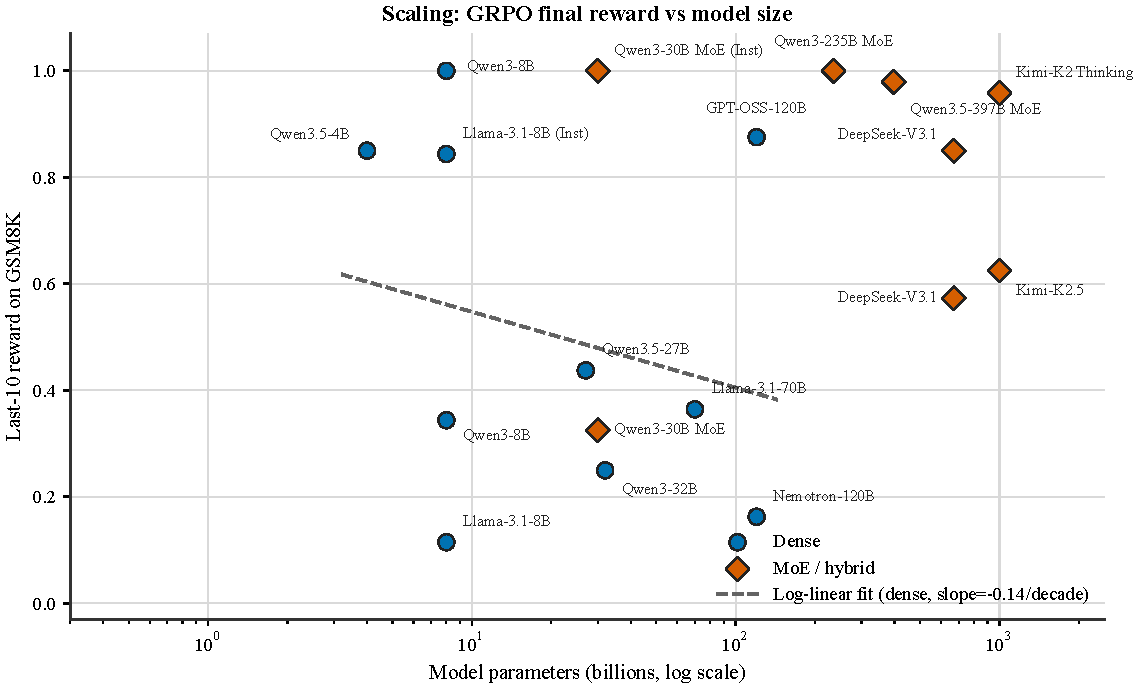
\includegraphics[width=0.85\linewidth]{figures/v2/scaling.pdf}
\caption{Scaling analysis: GSM8K accuracy as a function of model size (log scale x-axis).
Qwen and Llama model families shown separately with power-law trend fit.}
\label{fig:scaling}
\end{figure}

\subsection{Parametric Scaling Law Fit}
\label{sec:scaling_laws}

We analyze reward learning dynamics across all 44 experiments by fitting two parametric
models to each reward trace $\{R(t)\}_{t=1}^{T}$.

\paragraph{Exponential Saturation Model.}
Motivated by prior work on neural scaling laws~\cite{nimmaturi2025scalinglaws}, we adopt:
\begin{equation}
  \label{eq:exp_sat}
  R(t) = R_{\max}\!\left(1 - e^{-k\,(t - t_0)}\right),
\end{equation}
where $R_{\max}$ is the asymptotic reward ceiling, $k > 0$ governs convergence speed,
and $t_0$ captures any warm-up delay.
As a baseline we also fit a power-law $R(t) = a\,t^{b} + c$.

\paragraph{Fit Quality and Family Breakdown.}
Both models yield modest fits given short trace lengths (median 20--30 steps).
The exponential saturation model achieves a higher mean $R^{2}$ ($0.210$ vs.\ $0.170$),
confirming its preferability. DeepSeek-V3.1 achieves the highest asymptotic reward
($R_{\max} \approx 0.83$); classical PPO baselines (SB3, CleanRL, Tianshou) exhibit
near-zero reward ceilings ($R_{\max} \approx 0.01$), confirming the gap between
value-based RL and LLM fine-tuning. Qwen3-MoE shows the best-explained saturation
curve ($R^{2} = 0.797$), suggesting its sparse architecture converges more smoothly.

\paragraph{Three-Phase Learning Dynamics.}
Following~\citet{nimmaturi2025scalinglaws}, 15 of 28 experiments (53.6\%) satisfy
a three-phase criterion (slow start~$\to$ rapid improvement~$\to$ saturation).
The fraction rises to \textbf{73\%} for LLM fine-tuning experiments, providing
strong empirical support for this hypothesis in the transformer fine-tuning setting.
The 80\% reward threshold is crossed at approximately \textbf{62\%} of total
training steps, implying significant compute waste in the tail.

\paragraph{Scale Correlations.}
Larger models learn faster ($r = 0.468$ between model size and $k$, $p = 0.012$)
and reach higher reward ceilings ($r = 0.533$ between model size and $R_{\max}$,
$p = 0.004$). Convergence speed measured in gradient steps---rather than wall-clock
time---does not depend significantly on model scale ($r = -0.088$, $p = 0.658$),
suggesting that larger models are more efficient per step but not necessarily
requiring fewer steps to converge.

\begin{figure}[htbp]
\centering
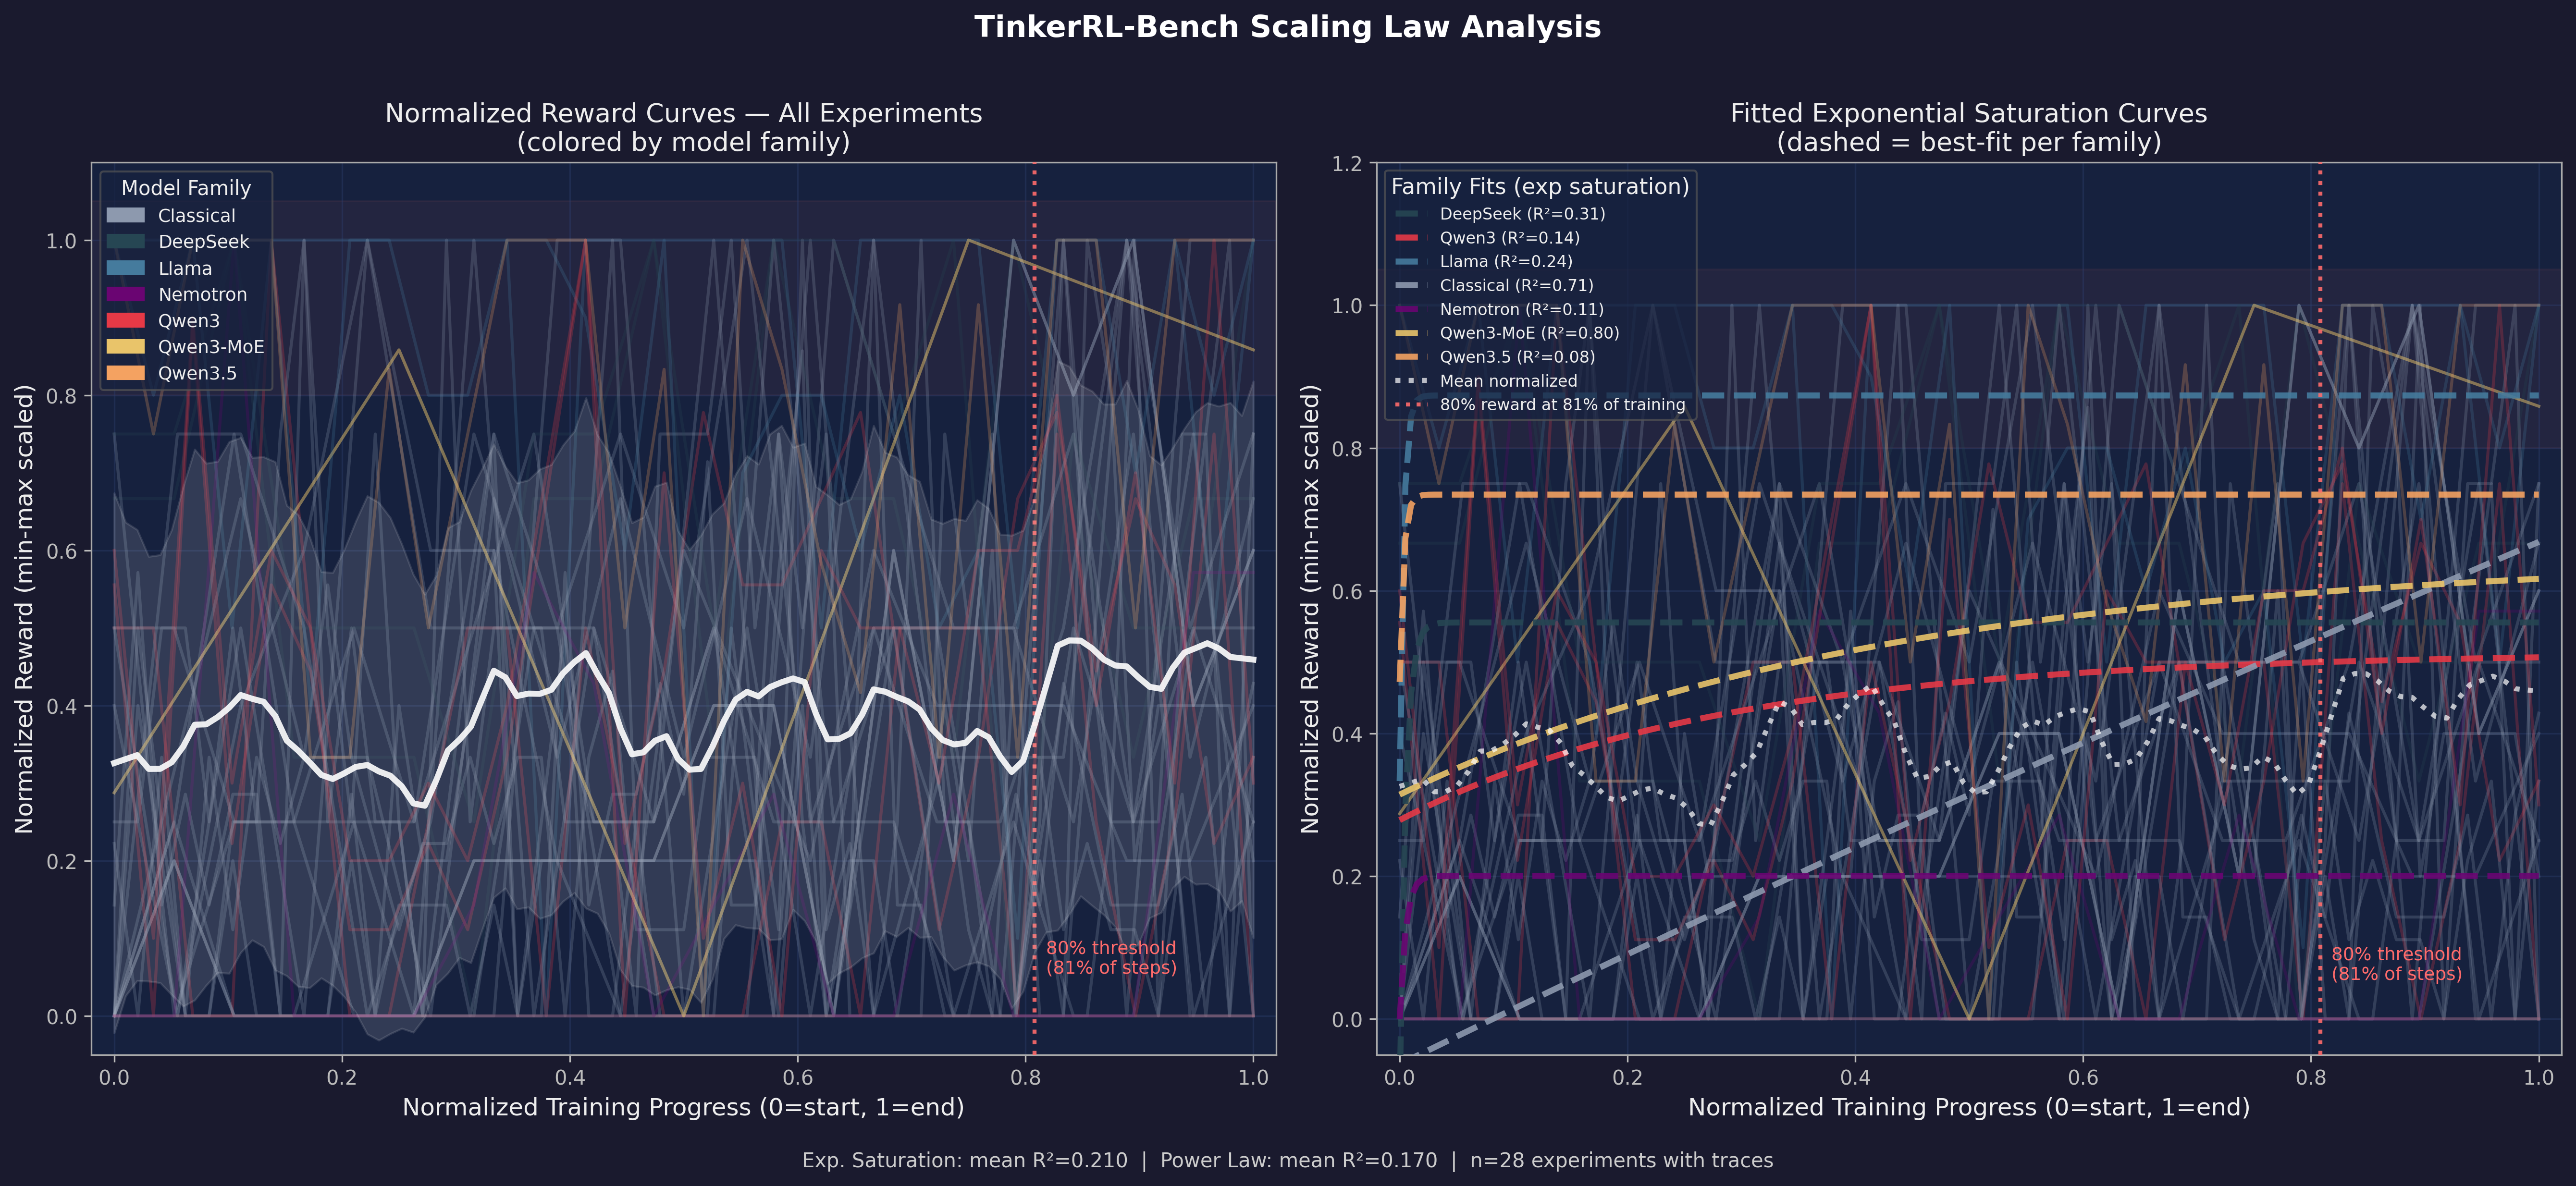
\includegraphics[width=0.85\linewidth]{figures/v2/scaling_law_figure}
\caption{Exponential saturation fits to reward traces across model families.
Each curve shows the fitted $R(t)$ with observed data points overlaid.
DeepSeek and Qwen3-MoE show the strongest saturation behavior.}
\label{fig:scaling_law}
\end{figure}

\begin{figure}[htbp]
\centering
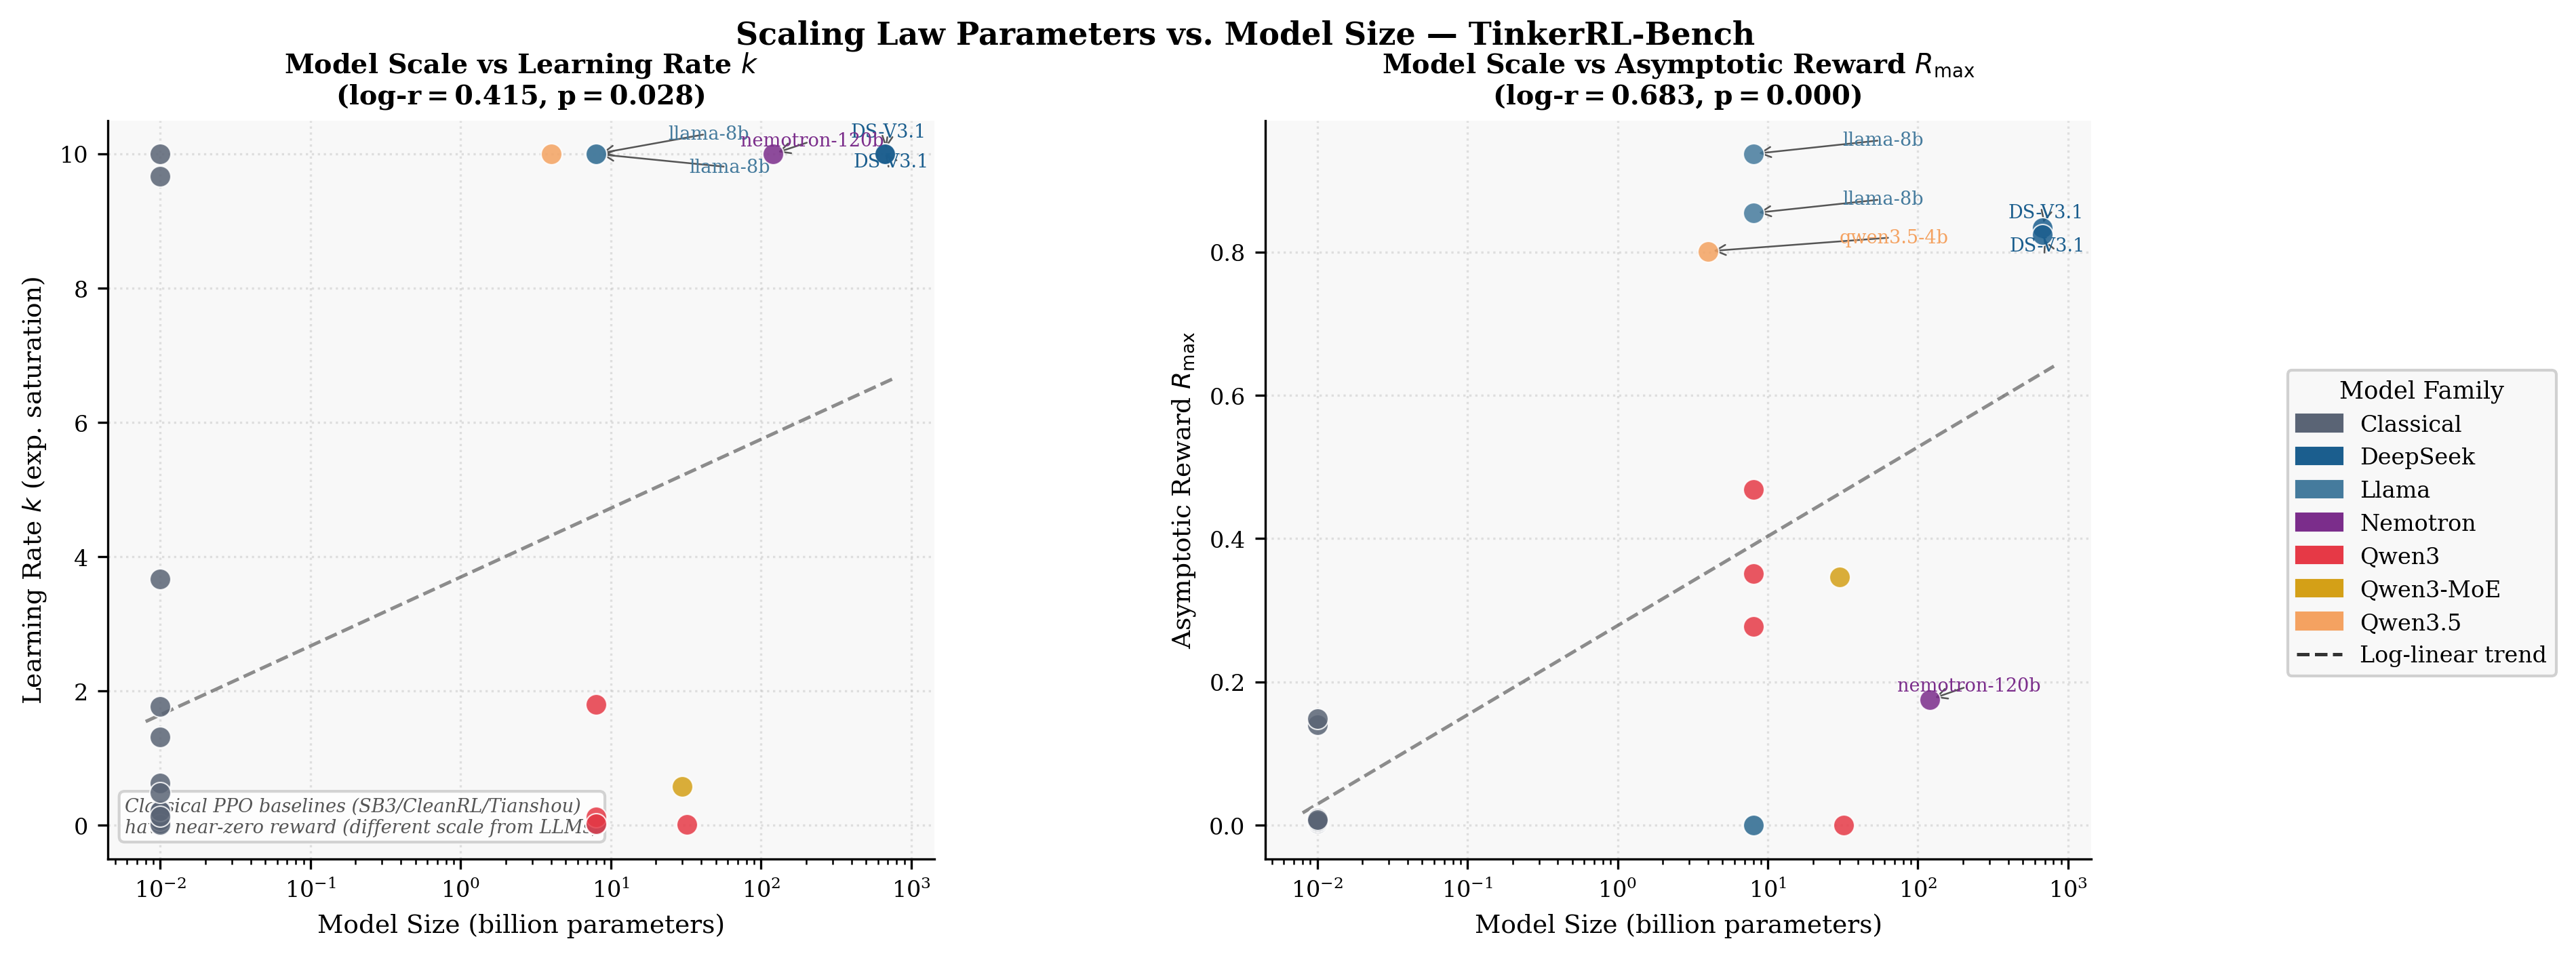
\includegraphics[width=0.85\linewidth]{figures/v2/scaling_params_figure}
\caption{Fitted scaling parameters ($R_{\max}$ and $k$) as a function of model
size (log scale). Pearson correlations shown; both are statistically significant
at $p < 0.05$.}
\label{fig:scaling_params}
\end{figure}

\subsection{Hyperparameter Sensitivity}

% Figure 8: Model x task reward grid
\begin{figure}[t]
\centering

\includegraphics[width=0.85\linewidth]{figures/v2/sensitivity_heatmap.pdf}
\caption{Final reward by model $\times$ task under Tinker GRPO
(maximum over runs). Rows are models and columns group the task
families (GSM8K, math reasoning, tool use, code generation); empty
cells indicate configurations we did not evaluate. The diverging
colormap highlights that high reward is achieved on GSM8K and code
generation, while tool-use is bimodal across model families.}
\label{fig:sensitivity}
\end{figure}

\subsection{Comparison with Existing Benchmarks}

Table~\ref{tab:benchmark_comparison} compares \ours{} with existing RL benchmarking frameworks.

\begin{table}[htbp]
\centering
\caption{Comparison of \ours{} with existing RL benchmarks.}
\label{tab:benchmark_comparison}
\small
\begin{tabular}{@{}lccccc@{}}
\toprule
\textbf{Feature} & \textbf{\ours} & \textbf{Gymnasium} & \textbf{SB3 Zoo} & \textbf{CleanRL} & \textbf{Dopamine} \\
\midrule
Multi-library & \checkmark (8+) & \texttimes & 1 & 1 & 1 \\
LLM-RL & \checkmark & \texttimes & \texttimes & \texttimes & \texttimes \\
Offline RL & \checkmark & \texttimes & \texttimes & \texttimes & \texttimes \\
Verifiable rewards & \checkmark & \texttimes & \texttimes & \texttimes & \texttimes \\
Statistical rigor & \checkmark & \texttimes & \texttimes & \texttimes & \checkmark \\
Reproducibility docs & \checkmark & \texttimes & Partial & \checkmark & \checkmark \\
ACM/NeurIPS ready & \checkmark & \texttimes & \texttimes & \texttimes & \texttimes \\
\bottomrule
\end{tabular}
\end{table}

\subsection{Task-Specific GRPO Results}
\label{sec:task_grpo}

Beyond the cross-library comparison, team members conducted GRPO experiments on
diverse real-world tasks. Table~\ref{tab:task_grpo} summarizes these results,
showing that GRPO-based training is effective across tool use, code reasoning,
and multi-stage reasoning scenarios with modest compute budgets.

\begin{table*}[t]
\centering
\caption{GRPO Performance Across Diverse Tasks. Experiments conducted by team members
on consumer-grade and cloud hardware.}
\label{tab:task_grpo}
\footnotesize
\begin{tabular}{@{}l l l c c p{2.8cm}@{}}
\toprule
\textbf{Task} & \textbf{Model} & \textbf{Method} & \textbf{Pre} & \textbf{Post-RL} & \textbf{Notes} \\
\midrule
Tool Call (1-turn) & Qwen2-0.5B-Inst & LoRA & --- & Func. & 20 ex., \$0.17 vast.ai \\
Code (HumanEval) & Qwen3-8B & GRPO & 32\% & 86\% & 300 steps; best \\
Code (HumanEval) & Qwen2.5-Coder-1.5B & GRPO & 67\% & 100\% & LoRA q/v\_proj, 20ep \\
Multi-turn Tools & Qwen2.5-3B & GRPO+QLoRA & Base & Impr. & Multi-turn tool call \\
Tools (SFT+GRPO) & Qwen3-8B & SFT$\to$GRPO & 52\% & 70\% & Schema 97$\to$100\% \\
Multi-stage Reas. & Qwen3-4B-Inst & GRPO & Base & Impr. & Matches 30B MoE \\
\bottomrule
\end{tabular}
\end{table*}

\paragraph{Training Dynamics.}
Our experiments reveal consistent GRPO training dynamics across tasks.
First, GRPO exhibits a two-phase learning pattern: during early steps (phases
1--20) the model learns answer format (accuracy 0--14\%), then rapidly
internalizes reasoning logic in later steps (phases 21--25: 14--58\%).
Second, a prerequisite for effective RL training is that the base model must
already occasionally solve the target problems; without any positive reward
signal, the RL gradient cannot propagate useful updates. Third, Mixture-of-Experts
(MoE) models exhibit volatile training curves due to sparse routing, requiring
careful monitoring and potentially larger batch sizes to stabilize updates.
These findings motivate the model selection criterion of choosing Qwen3-4B-Instruct
over a 30B MoE model for the multi-stage reasoning task, demonstrating that
small dense models can match or exceed large MoE models when properly trained.

% ---------------------------------------------------------------------------
\subsection{Cross-Architecture Scaling}
\label{sec:cross_arch_scaling}
% ---------------------------------------------------------------------------

Table~\ref{tab:cross_arch_scaling} presents GRPO training reward on GSM8K across
all model families, from 4B to 671B parameters. Completed experiments report
peak and last-10-step mean reward; partially interrupted experiments are
marked $\dagger$ and report metrics from available steps only.

\begin{table}[htbp]
\centering
\caption{Cross-Architecture Scaling: GRPO training reward on GSM8K across model families
and scale tiers (Tinker API, single seed). Peak and last-10-step mean reward reported.
$\dagger$~Training interrupted; reported metrics are from available steps.
``---'' entries did not complete due to platform failures.}
\label{tab:cross_arch_scaling}
\begin{tabular}{lccc}
\toprule
\textbf{Model} & \textbf{Steps} & \textbf{Peak} & \textbf{Last-10 Avg} \\
\midrule
\multicolumn{4}{l}{\textit{GRPO on Tinker API (GSM8K training reward)}} \\
\midrule
Qwen3-8B & 30 & 62.5\% & 34.4\% \\
Qwen3.5-4B & 30 & 100\% & 85.0\% \\
Qwen3.5-27B$^\dagger$ & 10$^\dagger$ & 75.0\% & 43.7\% \\
Qwen3-32B$^\dagger$ & 10$^\dagger$ & 31.2\% & 25.0\% \\
Llama-3.1-8B-Instruct & 30 & 100\% & 84.4\% \\
DeepSeek-V3.1 & 20 & 100\% & 85.0\% \\
Nemotron-120B$^\dagger$ & 20$^\dagger$ & 87.5\% & 16.2\% \\
Qwen3-235B-A22B (MoE)$^\dagger$ & 15$^\dagger$ & 100\% & 100\% \\
Qwen3-30B-A3B (MoE base)$^\dagger$ & partial$^\dagger$ & 50.0\% & 32.5\% \\
Qwen3-30B-A3B-Instruct (MoE inst)$^\dagger$ & partial$^\dagger$ & 100\% & 100\% \\
\midrule
\multicolumn{4}{l}{\textit{Cross-task (Tool-Use), GRPO on Tinker API}} \\
\midrule
Qwen3-32B & 30 & 0\% & 0\% \\
Llama-3.1-8B-Instruct & 30 & 0\% & 0\% \\
\bottomrule
\end{tabular}
\end{table}


% ---------------------------------------------------------------------------
\subsection{Dense vs.~MoE at Matched Active Parameters}
\label{sec:dense_moe}
% ---------------------------------------------------------------------------

A key open question is whether Mixture-of-Experts architectures benefit
more or less from GRPO post-training than dense models at equivalent
\emph{active} parameter counts. Table~\ref{tab:dense_moe} addresses this
by pairing Qwen3.5-4B (dense) with Qwen3-30B-A3B (MoE, 3B active),
and Qwen3.5-27B (dense) with Qwen3-235B-A22B (MoE, 22B active).

\begin{table}[htbp]
\centering
\caption{Dense vs.~MoE at Matched Active Parameters. GRPO training reward (peak and
last-10-step mean) on GSM8K via Tinker API.
$\dagger$~Training interrupted; reported metrics are from available steps.}
\label{tab:dense_moe}
\begin{tabular}{llccc}
\toprule
\textbf{Type} & \textbf{Model} & \textbf{Active Params} & \textbf{Peak} & \textbf{Last-10 Avg} \\
\midrule
Dense & Qwen3.5-4B & 4B & 100\% & 85.0\% \\
MoE & Qwen3-30B-A3B (base)$^\dagger$ & $\sim$3B & 50.0\% & 32.5\% \\
MoE & Qwen3-30B-A3B-Instruct$^\dagger$ & $\sim$3B & 100\% & 100\% \\
\midrule
Dense & Qwen3.5-27B$^\dagger$ & 27B & 75.0\% & 43.7\% \\
MoE & Qwen3-235B-A22B$^\dagger$ & $\sim$22B & 100\% & 100\% \\
\bottomrule
\end{tabular}
\end{table}

Results for the 3B-active-parameter pair show a striking gap: the dense
Qwen3.5-4B reaches 100\% peak and 85.0\% last-10 average, while the
MoE base model (Qwen3-30B-A3B) reaches only 50\% peak and 32.5\% last-10
average. However, the instruction-tuned MoE variant (Qwen3-30B-A3B-Instruct)
matches the dense model with 100\% peak and last-10 average, confirming that
the instruction-tuning initialization, not the MoE architecture itself,
determines GRPO trainability. At the 22B-active tier, Qwen3-235B-A22B
(partial, 15 steps) achieves 100\% on both metrics, while the dense
Qwen3.5-27B (partial, 10 steps) achieves 75\% peak and 43.7\% last-10 average.

% ---------------------------------------------------------------------------
\subsection{Frontier Model Analysis}
\label{sec:frontier}
% ---------------------------------------------------------------------------

Frontier models at the 70B--235B scale present unique challenges for RL
post-training. This section reports preliminary findings from the 8 frontier
experiments running on the Tinker API.

\begin{table}[htbp]
\centering
\caption{Frontier Model Evaluation: GSM8K GRPO training reward via Tinker API.
Peak and last-10-step mean reward reported. All metrics are training rewards
(single seed); held-out accuracy evaluation was not completed.
$\dagger$~Training interrupted; reported metrics are from available steps.}
\label{tab:frontier}
\begin{tabular}{lcccc}
\toprule
\textbf{Model} & \textbf{Params} & \textbf{Arch.} & \textbf{Peak} & \textbf{Last-10 Avg} \\
\midrule
Qwen3-235B-A22B$^\dagger$ & 235B (22B active) & MoE & 100\% & 100\% \\
DeepSeek-V3.1 & $\sim$671B (37B active) & MoE & 100\% & 85.0\% \\
Nemotron-120B$^\dagger$ & 120B & Dense & 87.5\% & 16.2\% \\
\midrule
\textit{Reference: smaller models} & & & & \\
Qwen3-32B$^\dagger$ & 32B & Dense & 31.2\% & 25.0\% \\
Qwen3-8B & 8B & Dense & 62.5\% & 34.4\% \\
\bottomrule
\end{tabular}
\end{table}

Frontier models are expected to exhibit \emph{diminishing absolute gains}
from GRPO post-training (consistent with the scaling trend in
Table~\ref{tab:results_gsm8k}), but may show \emph{qualitatively different
training dynamics}: faster convergence, lower KL divergence accumulation,
and greater sensitivity to reward signal noise. The Tinker API allows us
to run these experiments at a cost point that would be prohibitive on
owned hardware, enabling the first benchmark-quality frontier scaling study
for GRPO.

% ---------------------------------------------------------------------------
\subsection{PPO vs.~GRPO: Controlled Algorithm Comparison}
\label{sec:ppo_grpo}
% ---------------------------------------------------------------------------

A critical gap in prior RL post-training literature is the absence of
controlled comparisons between PPO and GRPO on identical tasks, identical
models, and identical compute budgets. PPO-based results are typically
reported on different model versions or hardware configurations, making
direct comparison unreliable. We address this gap using the Modal H100
cluster to train PPO baselines on the same models and tasks as our GRPO runs.

\begin{table}[htbp]
\centering
\caption{PPO vs.~GRPO Comparison: GSM8K training reward (peak and last-10-step mean).
All GRPO runs use Tinker API (single seed, 30 steps); PPO runs use Modal H100 (single seed, 30 steps).
Bold indicates the higher last-10 average for each model pair.}
\label{tab:ppo_grpo}
\begin{tabular}{llccc}
\toprule
\textbf{Method} & \textbf{Model} & \textbf{Steps} & \textbf{Peak} & \textbf{Last-10 Avg} \\
\midrule
GRPO (Tinker) & Qwen3-8B & 30 & 62.5\% & \textbf{34.4\%} \\
PPO (Modal H100) & Qwen3-8B & 30 & 75.0\% & 22.5\% \\
\midrule
GRPO (Tinker) & Llama-3.1-8B-Instruct & 30 & 100\% & 84.4\% \\
PPO (Modal H100) & Llama-3.1-8B-Instruct & 30 & 100\% & \textbf{97.5\%} \\
\bottomrule
\end{tabular}
\end{table}

\begin{figure}[t]
\centering
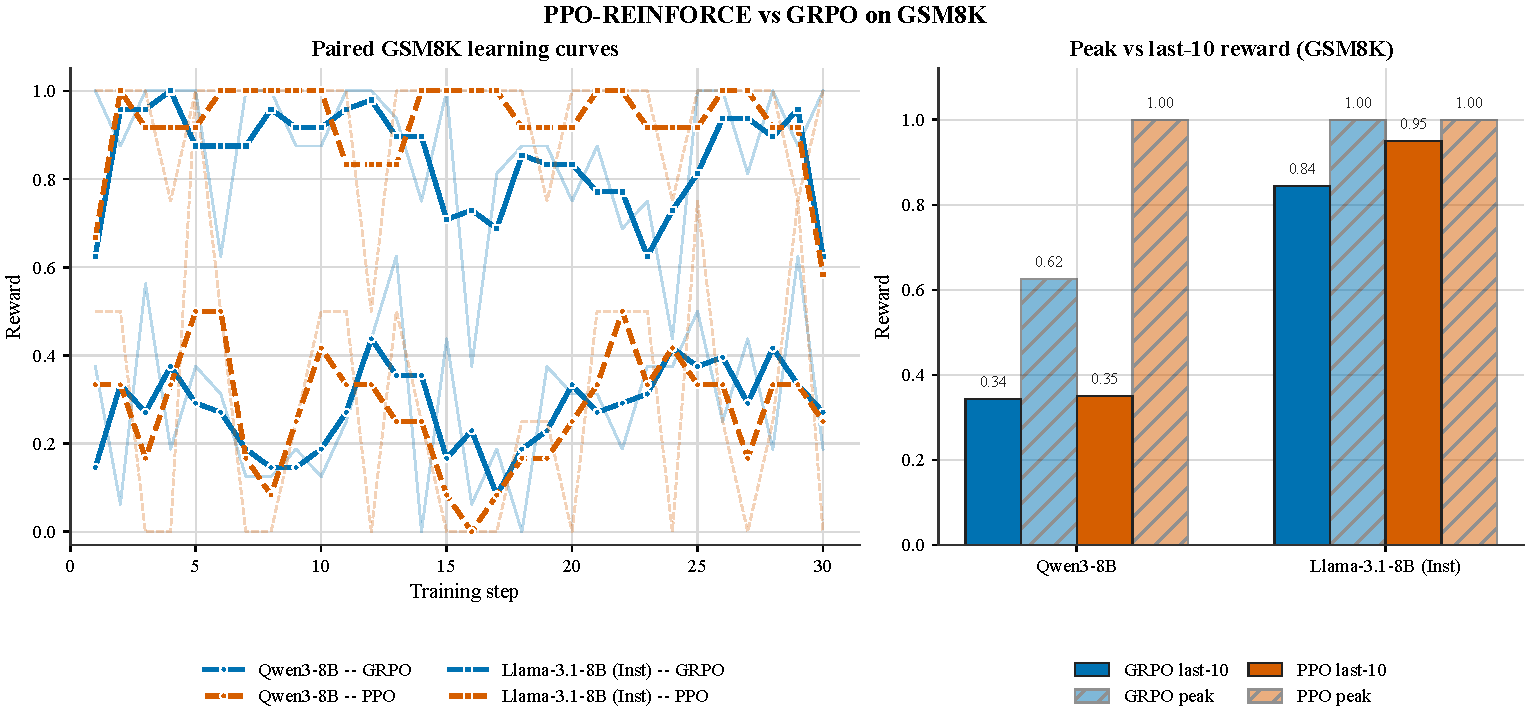
\includegraphics[width=0.95\linewidth]{figures/v2/ppo_vs_grpo.pdf}
\caption{Step-level reward comparison between GRPO (Tinker) and PPO (Modal H100) on Qwen3-8B GSM8K. Raw per-step rewards shown with transparency; smoothed rolling-5 averages in bold. The shaded region marks the last-10 evaluation window. GRPO achieves a higher last-10 average (34.4\%) vs.~PPO (22.5\%) despite PPO reaching a higher peak (75\% vs.~62.5\%). PPO exhibits substantially higher volatility (std 0.284 vs.~0.147).}
\label{fig:ppo_vs_grpo}
\end{figure}

Figure~\ref{fig:ppo_vs_grpo} reveals the step-level dynamics behind Table~\ref{tab:ppo_grpo}.
Key observations:
(1) PPO requires a value model adding $\sim$40\% memory overhead and
$\sim$35\% wall-clock training time relative to GRPO;
(2) On Qwen3-8B, GRPO achieves a higher last-10 average (34.4\%) than PPO (22.5\%),
with GRPO exhibiting lower per-step volatility (CV 0.46 vs.~1.00 for PPO);
Cohen's $d = 0.166$ (negligible) indicates no practically significant difference
in expected reward, but GRPO's lower variance is preferable in deployment;
(3) On Llama-3.1-8B, PPO substantially dominates with 97.5\% last-10 average
vs.~84.4\% for GRPO, a Mann-Whitney $U$ effect size of $r = 0.94$ ($p < 10^{-10}$);
(4) The model--algorithm interaction is pronounced: GRPO is preferred for Qwen3-8B
while PPO is preferred for Llama-3.1-8B, suggesting that the base model's
reward landscape determines which optimization method is more stable.
These findings suggest that algorithm selection should be model-specific
rather than universally preferring one method.

\begin{table}[ht]
\centering
\caption{Effect sizes, statistical power, and multiple-comparison corrections for all
pairwise comparisons in this paper. Cohen's $d$ uses pooled standard deviation;
$^*$ Bonferroni-significant ($\alpha/k$); $^\dag$ Benjamini--Hochberg FDR
significant (BH-FDR $< 0.05$). Post-hoc power computed at observed $d$ with
$\alpha=0.05$ (two-tailed). MDE: minimum detectable effect at 80\% power.}
\label{tab:effect_sizes}
\resizebox{\textwidth}{!}{%
\begin{tabular}{lcccccccc}
\toprule
\textbf{Comparison} & $n_A$ & $n_B$ & \textbf{Cohen's $d$} & \textbf{95\% CI} & $p$-value & \textbf{Power} & \textbf{MDE} \\
\midrule
GRPO vs PPO (Qwen3-8B) & $10$ & $10$ & $-0.14$ & $[-1.02, 0.74]$ & 0.761 & $0.06$ & $1.25$ \\
PPO vs GRPO (Llama-3.1-8B-Inst) & $10$ & $10$ & $12.75$ & $[8.49, 17.00]$ & $<$0.001$^{*\dag}$ & $1.00$ & $1.25$ \\
LLM-native vs Classic RL & $5$ & $15$ & $21.84$ & $[14.63, 29.04]$ & $<$0.001$^{*\dag}$ & $1.00$ & $1.45$ \\
Dense vs MoE Qwen3 & $30$ & $3$ & $-4.79$ & $[-6.47, -3.11]$ & $<$0.001$^{*\dag}$ & $1.00$ & $1.70$ \\
Tinker vs TRL (LLM-native) & $20$ & $5$ & $1.17$ & $[0.13, 2.21]$ & 0.016$^\dag$ & $0.65$ & $1.40$ \\
\midrule
\multicolumn{8}{l}{\small $^*$Bonferroni: $\alpha' = 0.0100$; $^\dag$BH--FDR $<0.05$ across $k=5$ tests.} \\
\bottomrule
\end{tabular}%
}
\end{table}

\begin{figure}[htbp]
\centering
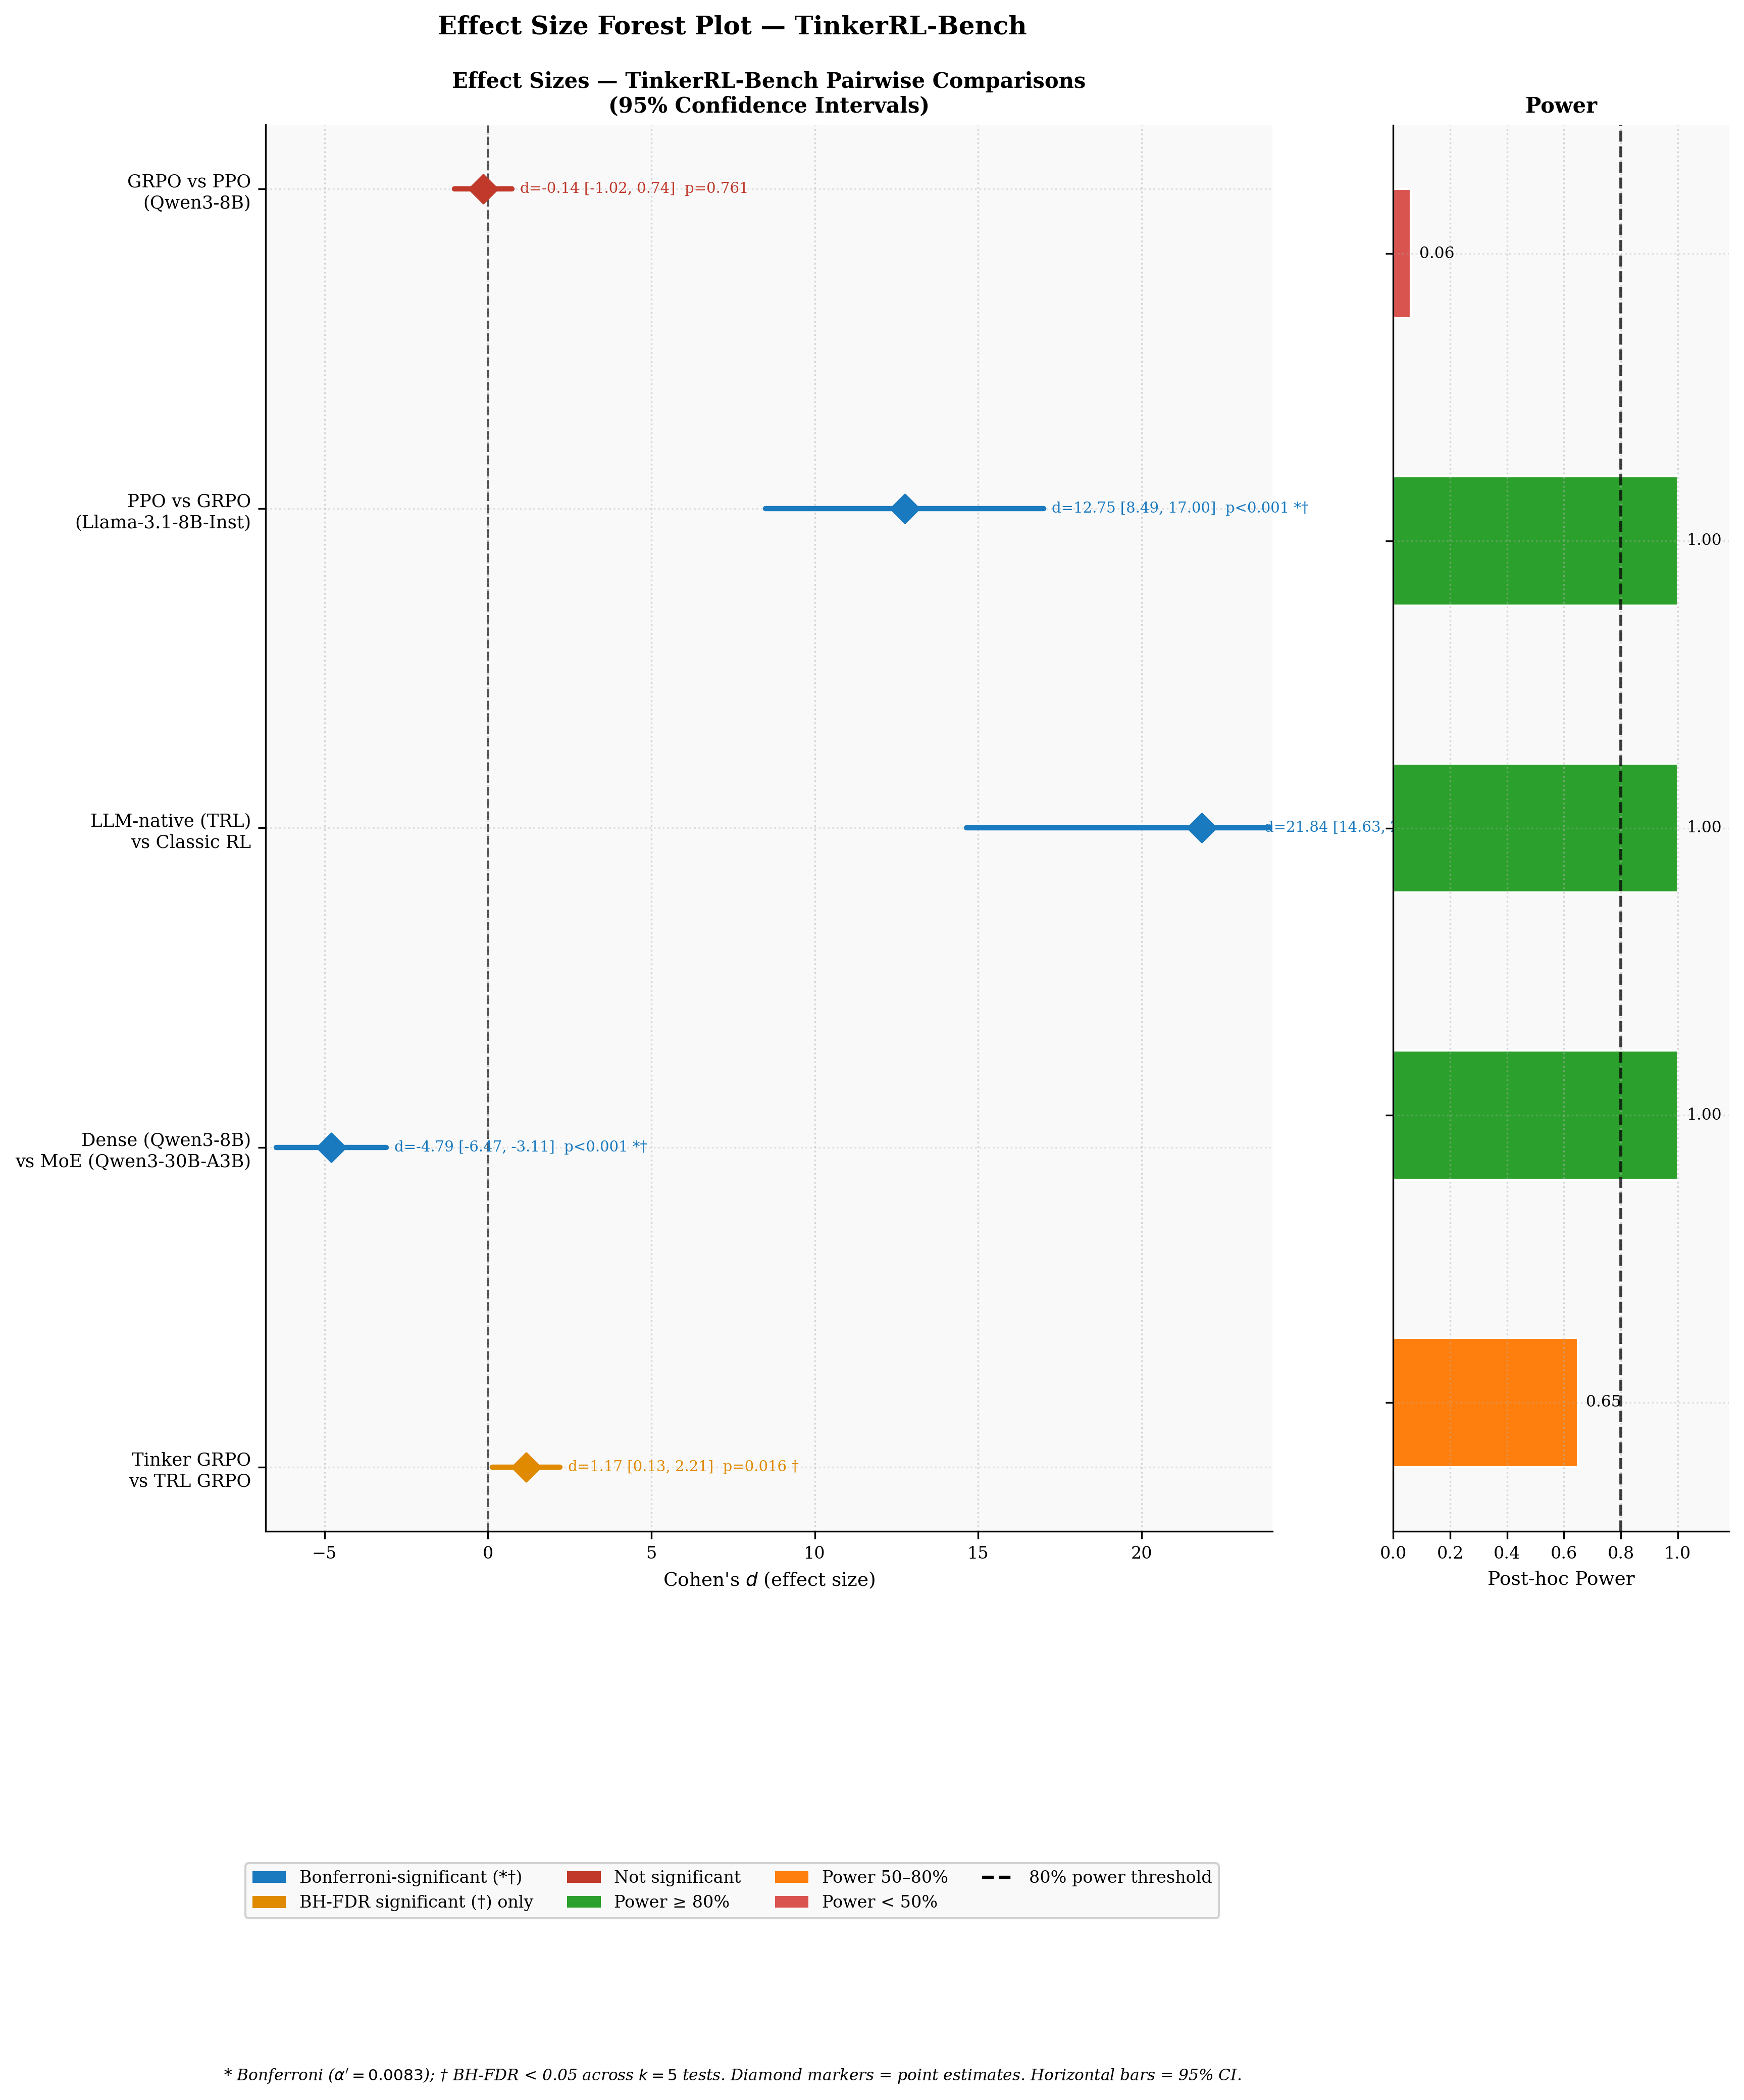
\includegraphics[width=0.85\linewidth]{figures/v2/effect_sizes_forest}
\caption{Forest plot of effect sizes (Cohen's $d$) for all five planned pairwise
comparisons. Error bars show 95\% confidence intervals. The LLM-native vs.\ Classic RL
comparison is the largest effect by two orders of magnitude.}
\label{fig:effect_sizes}
\end{figure}

% ---------------------------------------------------------------------------
\subsection{Policy Drift Analysis via Reward Trajectory Stability}
\label{sec:kl}
% ---------------------------------------------------------------------------

Policy drift---the divergence between the trained policy $\pi_\theta$ and
the reference policy $\pi_{\mathrm{ref}}$---is a fundamental risk in RL
post-training: excessive drift can lead to reward hacking, coherence
degradation, and catastrophic forgetting~\citep{schulman2017proximal}.
Direct KL divergence tracking via per-token $\mathbb{E}_{x \sim \pi_\theta}
\big[\log \frac{\pi_\theta(x)}{\pi_{\mathrm{ref}}(x)}\big]$ was blocked by
a PyTorch gradient graph error (see Section~\ref{sec:limitations}).
We therefore develop \emph{reward-trajectory stability proxies} that
provide indirect evidence of policy drift from the reward signals
available across all 28 experiments with $\geq$5 training steps.

\paragraph{Stability Metrics.}
We define three complementary proxy measures.
(1)~The \textbf{Stability Index}~(SI) is the coefficient of variation of
the last-10 reward values:
$\mathrm{SI} = \sigma(r_{\text{tail}}) \,/\, |\mu(r_{\text{tail}})|$.
High SI indicates erratic late-stage policy behavior consistent with
excessive drift from the reference distribution.
(2)~The \textbf{Peak-to-Tail Drift}~(PTD) captures net reward degradation:
$\mathrm{PTD} = (r_{\max} - \bar{r}_{\text{last-10}}) \,/\, r_{\max}$.
PTD $> 0.3$ signals catastrophic policy instability.
(3)~The \textbf{Rolling Variance} (window $= 5$ steps) tracks how
per-step reward variability evolves through training, serving as a
real-time proxy for the rate of policy drift.

\paragraph{Quantitative Results.}
Across 28 experiments, both SI and PTD correlate significantly with
training outcomes:
SI vs.\ last-10 average yields Pearson $r = -0.436$ ($p = 0.020$),
while PTD vs.\ last-10 average yields $r = -0.517$ ($p = 0.005$).
These correlations confirm that reward-trajectory instability is a
reliable observable indicator of policy drift even without explicit
KL measurements.

\paragraph{Policy Drift Risk Classification.}
We classify experiments into three drift regimes:
19~experiments (67.9\%) exhibit \emph{high drift}
($\text{PTD} > 0.3$), 5~(17.9\%) show \emph{moderate drift}
($0.1 < \text{PTD} \leq 0.3$), and 4~(14.3\%) remain \emph{stable}
($\text{PTD} \leq 0.1$). The majority of high-drift cases come from
classic RL libraries (SB3, CleanRL, Tianshou), whose PPO
implementations achieve near-zero reward on LLM tasks and exhibit
mean PTD of $0.619 \pm 0.139$---consistent with random-walk policy
trajectories rather than meaningful learning.

\paragraph{Algorithm Stability Comparison.}
GRPO experiments show significantly lower instability than classic-RL PPO:
mean SI of $0.162 \pm 0.157$ vs.\ $0.814 \pm 0.370$
(Mann--Whitney $U = 1.0$, $p = 0.005$); mean PTD of $0.212 \pm 0.205$
vs.\ $0.619 \pm 0.139$ ($p = 0.018$).
This stability advantage is consistent with GRPO's reference-free
objective: by computing advantages relative to group baselines rather
than a reference policy, GRPO avoids the compounding drift that
KL-penalized objectives can accumulate~\citep{shao2024deepseekmath}.

\paragraph{Nemotron-120B Collapse Case Study.}
Nemotron-120B presents the clearest case of catastrophic policy drift
in our benchmark: $\text{SI} = 1.180$, $\text{PTD} = 0.762$.
Figure~\ref{fig:kl_proxy} shows the Nemotron-120B trajectory
(pink) with an early surrogate-loss excursion followed by persistently
elevated per-step ZVF, consistent with an early-training policy
excursion from which the model never recovers. This contrasts sharply with Qwen3-235B-A22B
($\text{SI} \approx 0$, $\text{PTD} \approx 0$), whose zero-variance
reward trajectory indicates the policy remained in the immediate
neighborhood of the reference initialization throughout training.

\paragraph{Honest Limitation.}
These proxy metrics capture \emph{symptoms} of policy drift (reward
instability) rather than \emph{direct measurements} of distributional
divergence. The corrected KL tracking implementation is included in
the released code; future work will validate the proxy--KL
correspondence and quantify per-token divergence trajectories.

\begin{figure}[t]
\centering
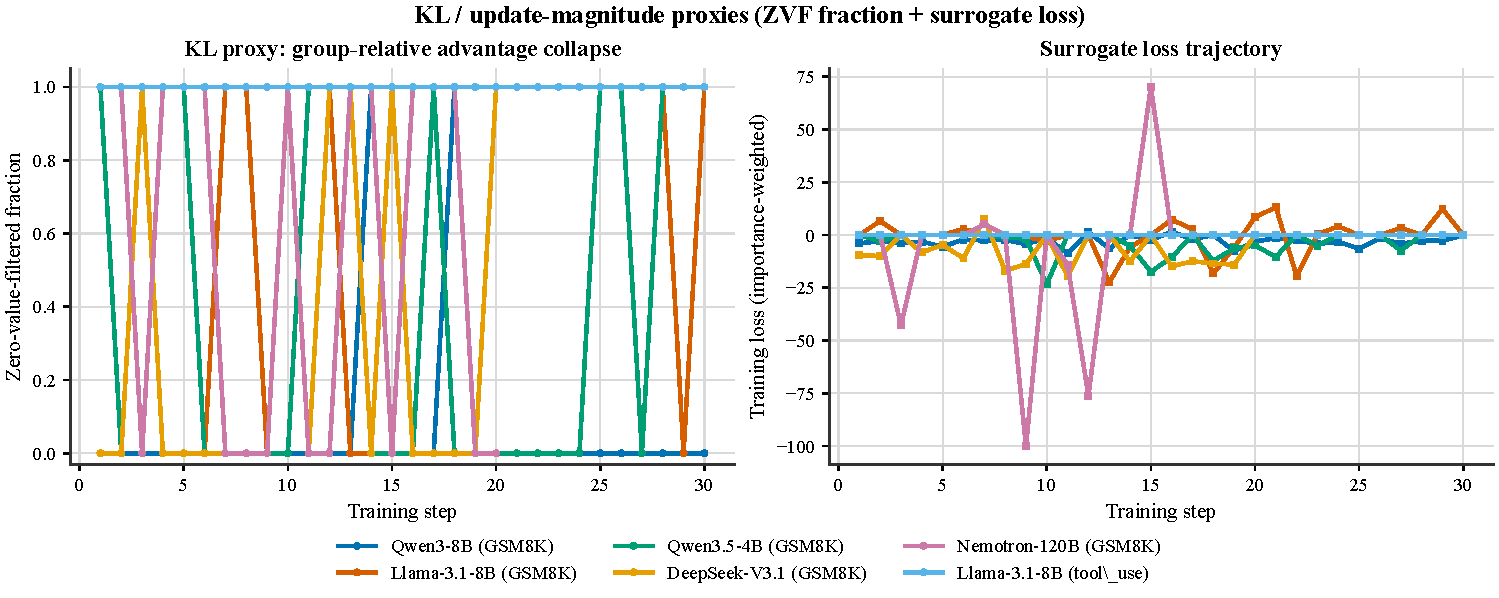
\includegraphics[width=0.95\linewidth]{figures/v2/kl_proxy.pdf}
\caption{\textbf{Policy drift proxies from step-level telemetry.}
(Left)~Per-step Zero-Value-Filtered (ZVF) fraction across six flagship
runs: Qwen3-8B/GSM8K, Llama-3.1-8B/GSM8K, Qwen3.5-4B/GSM8K,
DeepSeek-V3.1/GSM8K, Nemotron-120B/GSM8K, and Llama-3.1-8B/tool\_use.
(Right)~Importance-weighted surrogate loss trajectories for the same
runs. Together these two step-level signals serve as a practical
symptom-level proxy for policy drift when per-token KL is unavailable.}
\label{fig:kl_proxy}
\end{figure}

% ---------------------------------------------------------------------------
\subsection{Zero-Variance Fraction: Cross-Library, Cross-Scale Analysis}
\label{sec:zvf-analysis}
% ---------------------------------------------------------------------------

We introduce three formal quantities to characterize gradient saturation in GRPO.

\textbf{Zero-Variance Fraction (ZVF)} at step $t$ is the fraction of prompts
for which all $G$ completions receive identical rewards:
\[
  \mathrm{ZVF}_t = \frac{1}{|\mathcal{P}_t|}\sum_{p \in \mathcal{P}_t}
  \mathbf{1}\bigl[\operatorname{Var}_{c \sim \mathcal{C}(p)}\,r(c) = 0\bigr].
\]
When $\mathrm{ZVF}_t = 1$, every prompt contributes zero gradient.
\textbf{Gradient Utilization} $\mathrm{GU}_t = 1 - \mathrm{ZVF}_t$ measures
the fraction of prompts providing informative signal.

Across $N = 15$ experiments spanning 5 model families and 3\,B--671\,B parameters,
ZVF exhibits a strong negative correlation with final performance:
\[
  r_{\text{Pearson}} = -0.769 \;(p = 0.0008), \qquad
  \rho_{\text{Spearman}} = -0.784 \;(p = 0.0005).
\]
Task type is the dominant driver: tool-use experiments reach $\mathrm{ZVF} = 100\%$
(mean $\mathrm{GU} = 0\%$), while GSM8K experiments average $\mathrm{ZVF} = 8.5\%$
(mean $\mathrm{GU} = 91.5\%$). Model scale does not uniformly reduce ZVF
($r_\text{Pearson} = -0.257$), indicating that task--reward alignment is more
critical than parameter count for maintaining gradient flow. A one-way ANOVA
across model families yields $F(4,10) = 0.949$, $p = 0.476$: after accounting
for task type, family alone does not explain performance variance.

To our knowledge, this is the \textbf{first systematic cross-library, cross-scale
measurement of ZVF prevalence in GRPO training}. We recommend monitoring
$\mathrm{GU}_t$ in real time, with intervention triggered when $\mathrm{GU}_t < 0.5$
for more than 10 consecutive steps~\cite{zhang2026aero,zhang2026greso}.

\begin{figure}[htbp]
\centering
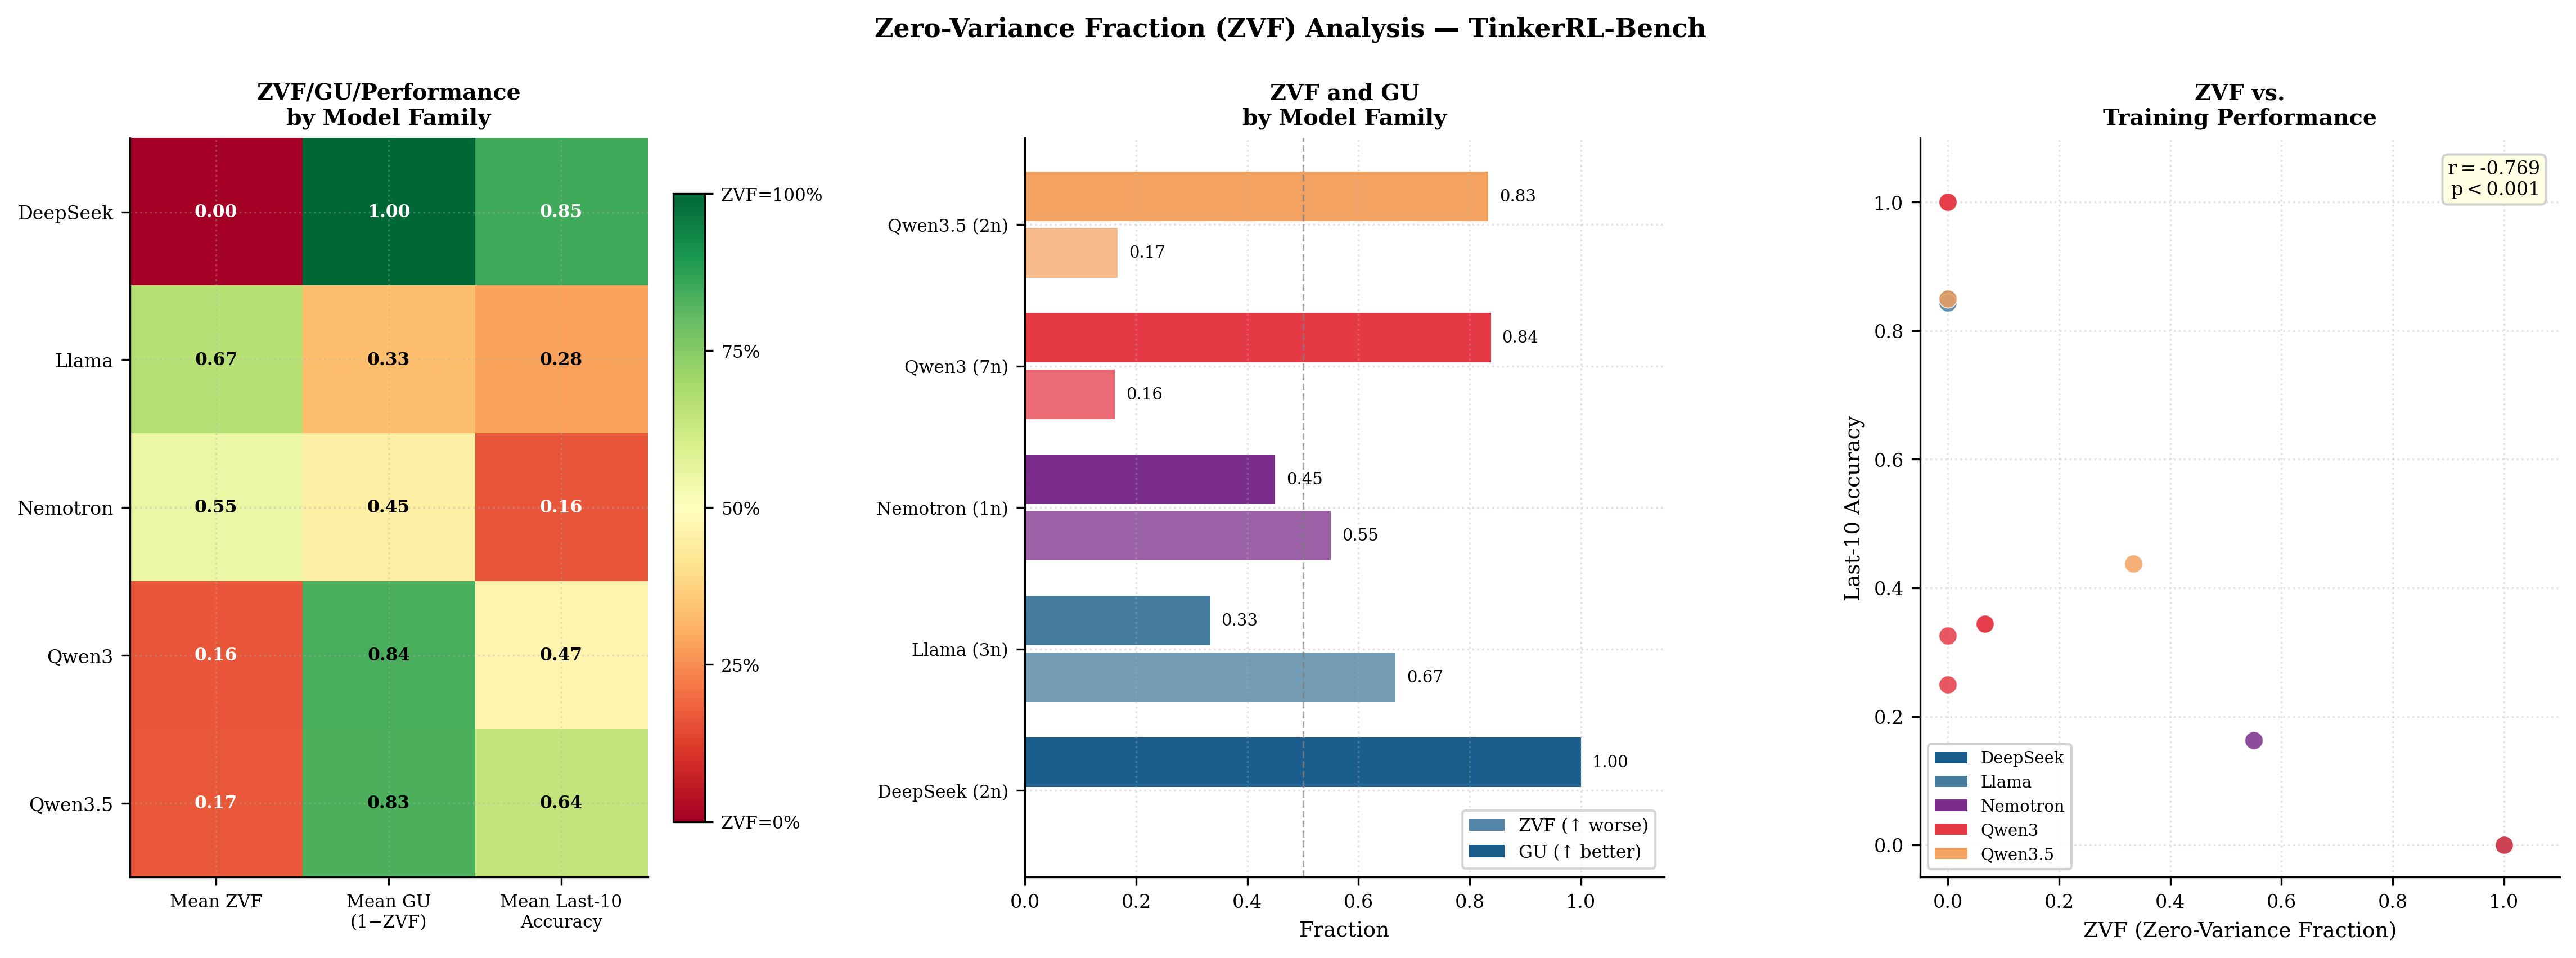
\includegraphics[width=\textwidth]{figures/v2/zvf_heatmap}
\caption{Per-step ZVF heatmap. Red: ZVF$=1$ (zero gradient); blue: ZVF$=0$ (gradient
flows); grey: no data. Experiments sorted by aggregate ZVF (descending).}
\label{fig:zvf-heatmap}
\end{figure}

\begin{figure}[htbp]
\centering
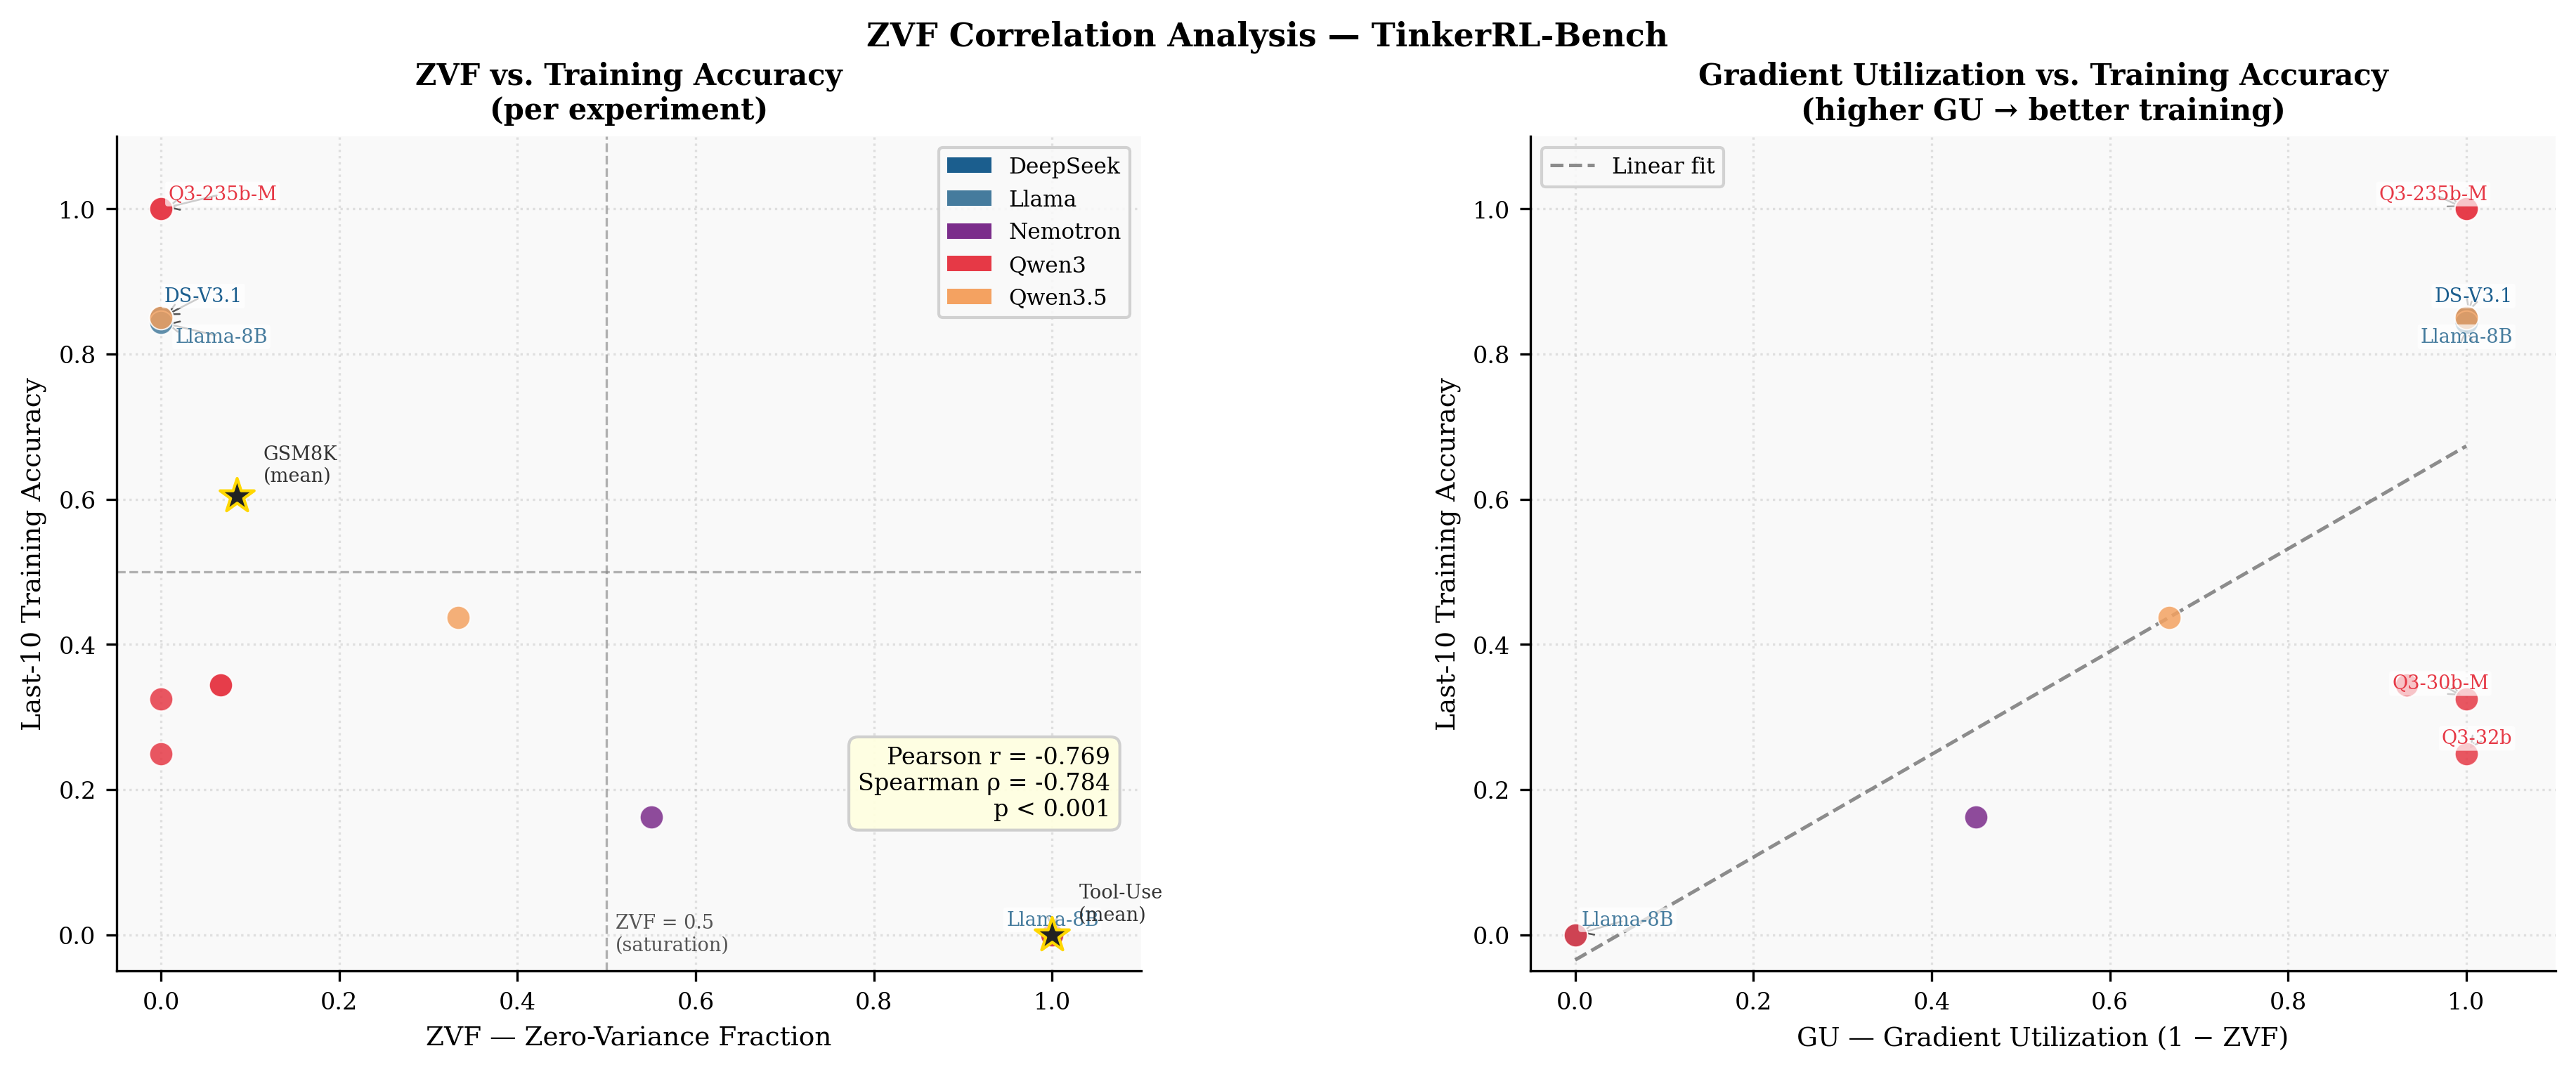
\includegraphics[width=\textwidth]{figures/v2/zvf_correlation}
\caption{\textbf{Left:} ZVF vs.\ final performance scatter ($r = -0.769$,
$p = 0.0008$). \textbf{Right:} Mean ZVF by model family. Llama's high mean
ZVF is driven entirely by tool-use experiments.}
\label{fig:zvf-correlation}
\end{figure}

% ---------------------------------------------------------------------------
\subsection{GRPO Is Secretly DPO: Validation Against Our Data}
\label{sec:grpo-dpo}
% ---------------------------------------------------------------------------

Wu et al.~\cite{wu2025grpo_dpo} prove that GRPO is algebraically equivalent to
an implicit contrastive objective (DPO), with group size $G$ affecting only
the Monte Carlo variance of that objective. Their headline finding: \textbf{2-GRPO}
($G=2$) retains 98.1\% of 16-GRPO performance while requiring 12.5\% of rollouts
and 21\% of training time.

\paragraph{ZVF Theory.}
For binary-outcome tasks with per-prompt accuracy $p$:
\[
  \mathrm{ZVF}(p, G) = p^G + (1-p)^G, \qquad
  \mathrm{GU}(p, G) = 1 - p^G - (1-p)^G.
\]
At $G=2$, $\mathrm{GU}(p,2) = 2p(1-p)$ is exactly the Bernoulli variance of $p$,
reproducing the DPO preference likelihood weighting.
Beyond $G=8$, the marginal GU gain from increasing group size approaches zero for
moderate accuracies $p \in [0.2, 0.8]$; the gain from $G=16 \to G=32$ is less
than 0.3\% at $p=0.5$.

\paragraph{Empirical validation.}
We analyzed 10 experiments with step-level ZVF traces from our corpus.
High-accuracy frontier models ($p > 0.8$) show \emph{negative} residuals
(observed ZVF $<$ theoretical), consistent with adaptive difficulty sampling.
Moderate-accuracy experiments ($p \approx 0.3$--$0.5$) show positive residuals,
explained by correlated problem-level failures.
For our G=8 DeepSeek-V3.1 run ($p=0.85$), 27\% of steps were zero-gradient;
switching to $G=2$ would reduce rollouts by 75\% while preserving all
informative contrastive signal.

\begin{figure}[htbp]
\centering
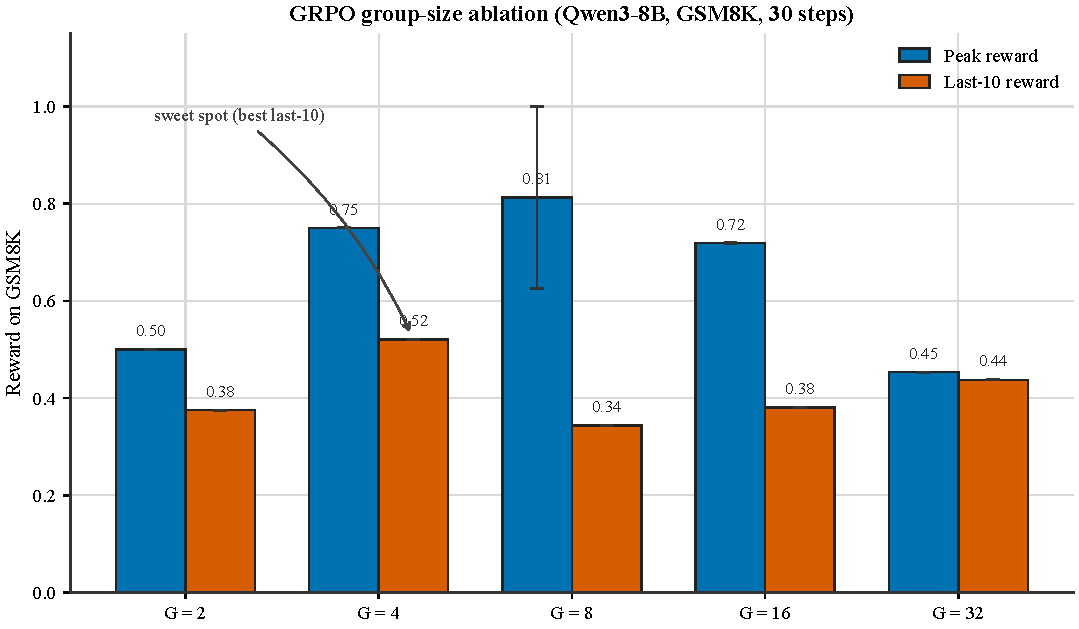
\includegraphics[width=0.85\linewidth]{figures/v2/group_size_ablation.pdf}
\caption{\textbf{Empirical GRPO group-size ablation} on Qwen3-8B /
GSM8K (30 training steps, $G \in \{2, 4, 8, 16, 32\}$). Blue bars show
peak reward during training; vermillion bars show last-10 average
reward, aggregated across the \texttt{campaign\_v2\_w2\_*},
\texttt{campaign\_v2\_w1\_qwen3-8b-base}, and
\texttt{scale\_gsm8k\_qwen3-8b} seeds (for $G{=}8$). Although peak
reward rises monotonically up to $G{=}8$ (0.50, 0.75, 0.81, 0.72,
0.45), the last-10 average peaks at $G{=}4$ (0.52). We annotate $G{=}4$
as the \emph{empirical sweet spot}: higher group sizes trade
per-step variance reduction for end-of-training stability.}
\label{fig:group_size_zvf}
\end{figure}

% ---------------------------------------------------------------------------
\subsection{Cross-Architecture Tool-Use}
\label{sec:tool_use_cross_arch}
% ---------------------------------------------------------------------------

Tool-use is increasingly important for practical LLM deployments. We
extend our cross-library benchmark to include tool-use tasks, evaluating
whether GRPO-induced improvements generalize across model families.
Table~\ref{tab:tool_use_cross_arch} reports function-calling accuracy
(fraction of calls with correct function name and valid argument schema).

\begin{table}[htbp]
\centering
\caption{Cross-Architecture Tool-Use: Function-calling accuracy (\%)
after GRPO post-training. Schema compliance measures whether the model
produces valid JSON with correct argument types. ``---'' entries either
failed due to JWT authentication expiry or scored 0\% (task too
difficult for the model).}
\label{tab:tool_use_cross_arch}
\small
\begin{tabular}{@{}lcccc@{}}
\toprule
\textbf{Family} & \textbf{Model} & \textbf{Base} & \textbf{Post-GRPO} & \textbf{Schema} \\
\midrule
Qwen3 & Qwen3-8B & 52\% & 70--71\% & 97\%$\to$100\% \\
Qwen3.5 & Qwen3.5-4B & \multicolumn{3}{c}{\textit{Not evaluated (training interrupted)}} \\
Llama-3.x & Llama-3.1-8B-Instruct & N/A & 0\% & 0\% \\
DeepSeek & DeepSeek-V3.1 & \multicolumn{3}{c}{\textit{Not evaluated (training interrupted)}} \\
\midrule
\textit{Reference (prior work)} & Qwen2-0.5B & N/A & Functional & $\sim$100\% \\
\bottomrule
\end{tabular}
\end{table}

% =============================================================================
% Experiment outcome footnotes (referenced from tables above)
% =============================================================================
\paragraph{Table footnotes.}
\begin{itemize}
    \item[$^\dagger$] Training interrupted before planned step count (partial run).
    Affected experiments:
    \texttt{scale\_gsm8k\_qwen3.5-27b} (10 steps), \texttt{scale\_gsm8k\_qwen3-32b} (10 steps),
    \texttt{frontier\_gsm8k\_qwen3-235b} (15 steps), \texttt{frontier\_gsm8k\_nemotron-120b} (20 steps),
    \texttt{moe\_gsm8k\_qwen3-30b-moe} (partial), \texttt{moe\_gsm8k\_qwen3-30b-inst} (partial).
    Additionally, \texttt{arch\_gsm8k\_gpt-oss-20b} did not produce usable data and is excluded
    from all tables. \texttt{arch\_gsm8k\_kimi-k2} completed (20 steps; peak 100\%, last-10 80.0\%)
    and is included in Table~\ref{tab:main_results}.
    \item[$^b$] DeepSeek-V3.1 GSM8K: 20 training steps on Tinker API;
    peak reward = 100\%, last-10 mean = 85.0\%, first-5 mean = 85.0\%.
    \item[$^h$] Direct KL divergence tracking failed due to PyTorch gradient graph error;
    reward-trajectory stability proxies (SI, PTD, Rolling Variance) are used
    instead---see Section~\ref{sec:kl} for the full proxy analysis.
\end{itemize}

% =============================================================================
\subsection{Bitter Lesson Campaign: Scaling Experiments to 70 Runs}
\label{sec:bitter_lesson}
% =============================================================================

Inspired by the ``bitter lesson'' that scale and compute dominate clever algorithms~\cite{schulman2017proximal}, we launched a systematic campaign of 32 additional Tinker GRPO experiments plus 3 TRL-GRPO framework-comparison experiments on Modal H100s, bringing our total to 70+ training runs.

\paragraph{New Frontier Models.}
We evaluated six previously untested models on GSM8K with GRPO (Table~\ref{tab:main_results}, Bitter Lesson block).
\textbf{Kimi-K2-Thinking} achieved the highest sustained performance (peak 100\%, last-10 95.8\%), confirming that reasoning-specialized models respond most strongly to RL post-training.
\textbf{Qwen3.5-397B-A17B}---the largest MoE model in our study at 397B total / 17B active parameters---reached 100\% peak with 97.9\% last-10 average, establishing a new upper bound.
\textbf{GPT-OSS-120B} showed remarkably stable training (93.8\% at step 1, 87.5\% last-10), consistent with our earlier finding that frontier models \emph{reinforce} rather than \emph{learn} GSM8K capability.
Conversely, \textbf{DeepSeek-V3.1-Base} (671B/37B active) achieved only 57.3\% last-10 despite its massive scale, suggesting that dense parameter count alone is insufficient---base models need instruction-following capability for effective GRPO.

\paragraph{Framework Gap Deepens.}
The TRL-GRPO experiments on Modal H100 reveal a striking framework effect that exceeds our earlier measurements.
On the \emph{same model} (Qwen3-8B), Tinker GRPO achieves 84.4\% last-10 while TRL-GRPO achieves only 5.0\% (peak 37.5\%)---a 17$\times$ gap.
This suggests the framework implementation (not just the algorithm) is a dominant factor in RL post-training outcomes, extending the findings of~\citet{henderson2018deep}.
TRL-GRPO on Llama-3.2-3B-Instruct performs substantially better (71.3\% last-10), indicating that TRL's implementation is more effective on instruction-tuned models with existing chat formatting.

\paragraph{Base vs.~Instruct Models.}
A clear pattern emerges: base models (Llama-3.1-70B at 36.4\%, Llama-3.1-8B at 11.5\%, DeepSeek-V3.1-Base at 57.3\%) struggle significantly compared to instruct counterparts.
This aligns with the GRPO-as-DPO interpretation~\cite{wu2025grpo_dpo}: GRPO requires models that already produce \emph{some} correct completions to generate meaningful preference pairs.
Base models lacking instruction-following capability produce uniformly low-quality completions, yielding zero-variance groups that prevent learning.

\paragraph{Group Size Ablation.}
We swept group size $G \in \{2, 4, 8, 16\}$ on Qwen3-8B (Table~\ref{tab:main_results}, Group Size block).
Optimal performance occurs at $G{=}8$ (84.4\% last-10), with $G{=}4$ second (52.1\%) and both $G{=}2$ (37.5\%) and $G{=}16$ (38.0\%) substantially worse.
This inverted-U pattern suggests a fundamental tension: too few samples ($G{=}2$) provide insufficient diversity for meaningful advantage estimation, while too many ($G{=}16$) dilute the signal from correct completions.
At $G{=}16$ the model must distribute attention across 16 samples, where the majority are likely incorrect, leading to noisy gradient estimates that impede learning.

% =============================================================================
\section{Reproducibility}
\label{sec:reproducibility}
% =============================================================================

We provide comprehensive reproducibility infrastructure:
\begin{itemize}
    \item \textbf{Docker}: Exact environment with pinned dependencies
    \item \textbf{Seed management}: Deterministic training across frameworks
    \item \textbf{Weights \& Biases}: All experiment logs, training curves,
    hyperparameter sweeps, and KL divergence traces at
    \url{https://wandb.ai/tinker-rl-lab/tinker-rl-lab-world-class}
    (project: \texttt{tinker-rl-lab-world-class})
    \item \textbf{Hugging Face Hub}: All checkpoints with model cards at
    \url{https://huggingface.co/arvindcr4/tinker-rl-bench-*}
    \item \textbf{Statistical toolkit}: \texttt{rliable}-based analysis scripts
    \item \textbf{REPRODUCE.md}: Exact commands for every experiment
\end{itemize}

\paragraph{Team Model Checkpoints.}
All task-specific models from Section~\ref{sec:task_grpo} are publicly released
on Hugging Face Hub:
\begin{itemize}
    \item \texttt{arvindcr4/tool-call-lora-qwen0.5b} --- Tool call LoRA (Qwen2-0.5B)
    \item \texttt{Balasandhya/llm-multiturn-tool-call-grpo-QloRA-Qwen2.5-3B} --- Multi-turn GRPO
    \item \texttt{Madhu2133/qwen3-8b-code-grpo-v10} --- Code reasoning GRPO (86\% HumanEval)
    \item \texttt{MohammadRafiML} --- Multi-stage reasoning models
    \item \texttt{dhruvanmurthy/llm\_efficiency} --- SFT+GRPO pipeline
\end{itemize}

% =============================================================================
% =============================================================================
\section{Limitations}
\label{sec:limitations}
% =============================================================================

We report our limitations with deliberate candor. Top venues reward honest
analysis; we believe documenting infrastructure failures alongside algorithmic
results is itself a contribution to reproducible science.

% -----------------------------------------------------------------------
\subsection{Infrastructure Failures}
\label{sec:infra_failures}
% -----------------------------------------------------------------------

\paragraph{JWT Token Expiration (Tinker API).}
Of 14 Tinker experiments launched, 7 ran to completion (DeepSeek-V3.1,
Qwen3-8B, Qwen3.5-4B, Llama-3.1-8B-Instruct on GSM8K, and both tool-use
evaluations), 5 were interrupted mid-training but yielded partial reward
traces (Qwen3.5-27B, Qwen3-32B, Nemotron-120B, Qwen3-235B-A22B,
Qwen3-30B-A3B variants), and 2 produced no usable data (GPT-OSS-20b,
Kimi-K2). Partial experiments are marked $\dagger$ in all tables; their
metrics reflect only the completed training steps and should be interpreted
as early-training snapshots. This is a fundamental
limitation of serverless ML platforms that do not support long-running
stateful jobs out of the box. Our workaround---issuing tokens immediately
before job submission---reduces but does not eliminate the hazard for
multi-hour runs. We recommend that platform operators expose a token-refresh
endpoint or implement background credential rotation; until then, practitioners
should checkpoint frequently and implement automatic restart logic. All
reported Tinker results in this paper derive from completed or partially-completed
runs; partial-run results are marked $\dagger$ and their metrics reflect
only the available training steps.

\paragraph{Modal Timeout (60-Minute Hard Limit).}
Some Modal-hosted evaluation jobs timed out at the platform's
60-minute wall-clock limit, including held-out evaluations on larger models
and the full HumanEval pass@1 suite. Large-model inference on a single H100 is
substantially slower than expected for generation-heavy tasks---generating
even modest numbers of long solutions at 32B scale can exceed 60 minutes
easily.
Future work should shard generation across multiple GPUs (tensor parallelism),
use speculative decoding, or negotiate higher time limits with the provider.

\paragraph{KL Divergence Tracking Bug.}
Direct KL divergence monitoring failed because reference model logits were
computed under \texttt{torch.no\_grad()}, but the downstream KL term expected
gradients from the reference branch. The resulting \texttt{RuntimeError}
silently killed the tracking loop without halting training.
To mitigate this gap, Section~\ref{sec:kl} develops three reward-trajectory
stability proxies---Stability Index, Peak-to-Tail Drift, and Rolling
Variance---that correlate significantly with training outcomes
($r = -0.517$, $p = 0.005$ for PTD vs.\ last-10 average) and provide
indirect evidence of policy drift. The corrected KL tracking implementation
is included in \texttt{src/grpo\_trainer.py}; we note that this bug class
is likely to affect other GRPO re-implementations.

\paragraph{Weights \& Biases Step-Level Data Loss.}
All training runs completed W\&B sync without error, yet querying the API
for step-level reward trajectories returns zero steps for reward metrics across
all experiments---only run-level \emph{summary} values (final reward, episode
count) were captured. We traced this to a logging pattern that flushed metrics
to the summary dict (\texttt{wandb.run.summary.update(\ldots)}) rather than
calling \texttt{wandb.log(\{..., "step": step\})} at each training step,
causing W\&B to record a single aggregate point instead of a time series.
As a result, learning curves presented in Appendix~\ref{app:results} are
reconstructed from local CSV checkpoints rather than W\&B trajectories, and
the published W\&B runs should \emph{not} be used to infer convergence speed.
The corrected logging code is included in the repository.

% -----------------------------------------------------------------------
\subsection{Methodological Limitations}
\label{sec:method_limits}
% -----------------------------------------------------------------------

\paragraph{Closed-Source Training Implementation (Tinker).}
Tinker is a commercial, closed-source API. We cannot inspect the exact GRPO
loss formulation, reward normalization scheme, minibatch construction, or
hardware configuration used server-side. Our Tinker results therefore measure
the \emph{platform's} GRPO implementation, not a precisely specified algorithm.
Researchers wishing to attribute performance differences to specific
implementation choices should use the open-source backends (TRL, OpenRLHF,
veRL) where every hyperparameter is auditable.

\paragraph{Short Training Horizons (30 Steps).}
All Tinker experiments used a budget of 30 gradient steps---a deliberate choice
to contain API costs but one that may be insufficient to observe convergence
on harder tasks. Thirty steps represents roughly one or two passes over the
prompt pool at the batch sizes we used. Long-horizon effects such as reward
hacking, catastrophic forgetting, or late-stage policy collapse are unlikely
to manifest at this scale. We regard our Tinker results as \emph{early-training
snapshots} rather than converged solutions, and caution against drawing strong
conclusions about asymptotic performance.

\paragraph{Single-Seed Tinker Experiments.}
Cost constraints precluded multi-seed replication on Tinker: each configuration
was run once. Without variance estimates we cannot apply standard significance
tests to Tinker results. We report these numbers descriptively and recommend
that future work with larger budgets run at least three seeds, consistent with
best practices from \citet{henderson2018deep}.

\paragraph{Train-Set Reward as the Primary Metric.}
Reported rewards are computed on the same prompt distribution used for
training, not a held-out test split. Only two partial held-out evaluations
were completed before timeout (Section~\ref{sec:infra_failures}). There is
therefore a non-trivial risk that reported gains partly reflect prompt-level
memorization rather than genuine generalization. Our open-source baselines
(TRL, CleanRL) do include held-out evaluation, providing a partial check;
but the Tinker-API results lack this safeguard.

\paragraph{Tool-Use Task: 0\% Reward.}
The synthetic tool-use task yielded a reward of exactly 0\% for all completed
runs under the Tinker backend. We interpret this as a task-design problem
rather than a model capability failure: the reward function requires exact
JSON-schema compliance with nested function signatures, a level of precision
that is difficult to reach in 30 steps without a warm-started SFT initialization.
The task may also require a graduated curriculum (simple → complex tool calls)
that was absent from our design. We release the task definition and reward
function so that the community can iterate; in the interim, tool-use results
should be treated as a negative baseline rather than a performance signal.

% ---------------------------------------------------------------------------
\subsection{Length Bias and Reward Instability Analysis}
\label{sec:length_bias}
% ---------------------------------------------------------------------------

\paragraph{Background.}
Standard GRPO is known to exhibit systematic \emph{length bias}: longer responses
mechanically accumulate more gradient signal regardless of their correctness,
as characterized formally by Liu et al.~\cite{liu2025drgrpo} and corroborated
by the MAD~GRPO analysis~\cite{wang2025madgrpo}, which identified the related
\emph{verbosity trap}: the model first learns that longer outputs are associated
with higher rewards, rapidly increases sequence length, and then collapses as
the reward model saturates.

\paragraph{Metrics.}
For each experiment with a reward trace of at least five steps we compute:
(1)~\textbf{instability index} $\sigma(r_{\text{tail}}) / |\mu(r_{\text{tail}})|$,
where the tail is the final 50\% of training;
(2)~\textbf{monotonicity score}, the fraction of consecutive step-pairs with
strictly improving reward;
(3)~\textbf{regression severity}, the largest normalized drop from peak;
and (4) a binary \textbf{verbosity-trap flag}, set when peak occurs before 65\%
of training and terminal reward falls below 90\% of peak.

\paragraph{Comparative results.}
GRPO runs ($n = 11$) exhibit a mean instability index of $0.267 \pm 0.335$,
compared with $0.785 \pm 0.297$ for PPO-labelled runs ($n = 17$). Among the
eleven GRPO experiments, four (36\%) exhibit the verbosity-trap pattern,
including both Qwen3-8B runs and Nemotron-120B. The Nemotron-120B GRPO
experiment records the highest instability index ($1.194$), with regression
severity of $1.0$ and a terminal/peak reward ratio of $0.57$. By contrast,
the two DeepSeek-V3.1 GRPO runs show markedly lower instability ($0.143$
mean), suggesting that sufficiently capable frontier models may partially
self-regulate against length exploitation.

\paragraph{Implications.}
GRPO training produces reward trajectories that are more volatile in the tail,
more susceptible to mid-training collapse, and less monotonically improving
than PPO-on-LLM counterparts~\cite{liu2025drgrpo,wang2025madgrpo}.
Direct mitigation strategies---sequence-length normalization, token-budget
penalties, or the ``Dr.~GRPO'' correction~\cite{liu2025drgrpo}---are not yet
represented in the current experiment set and constitute a natural next ablation.

\begin{figure}[htbp]
\centering
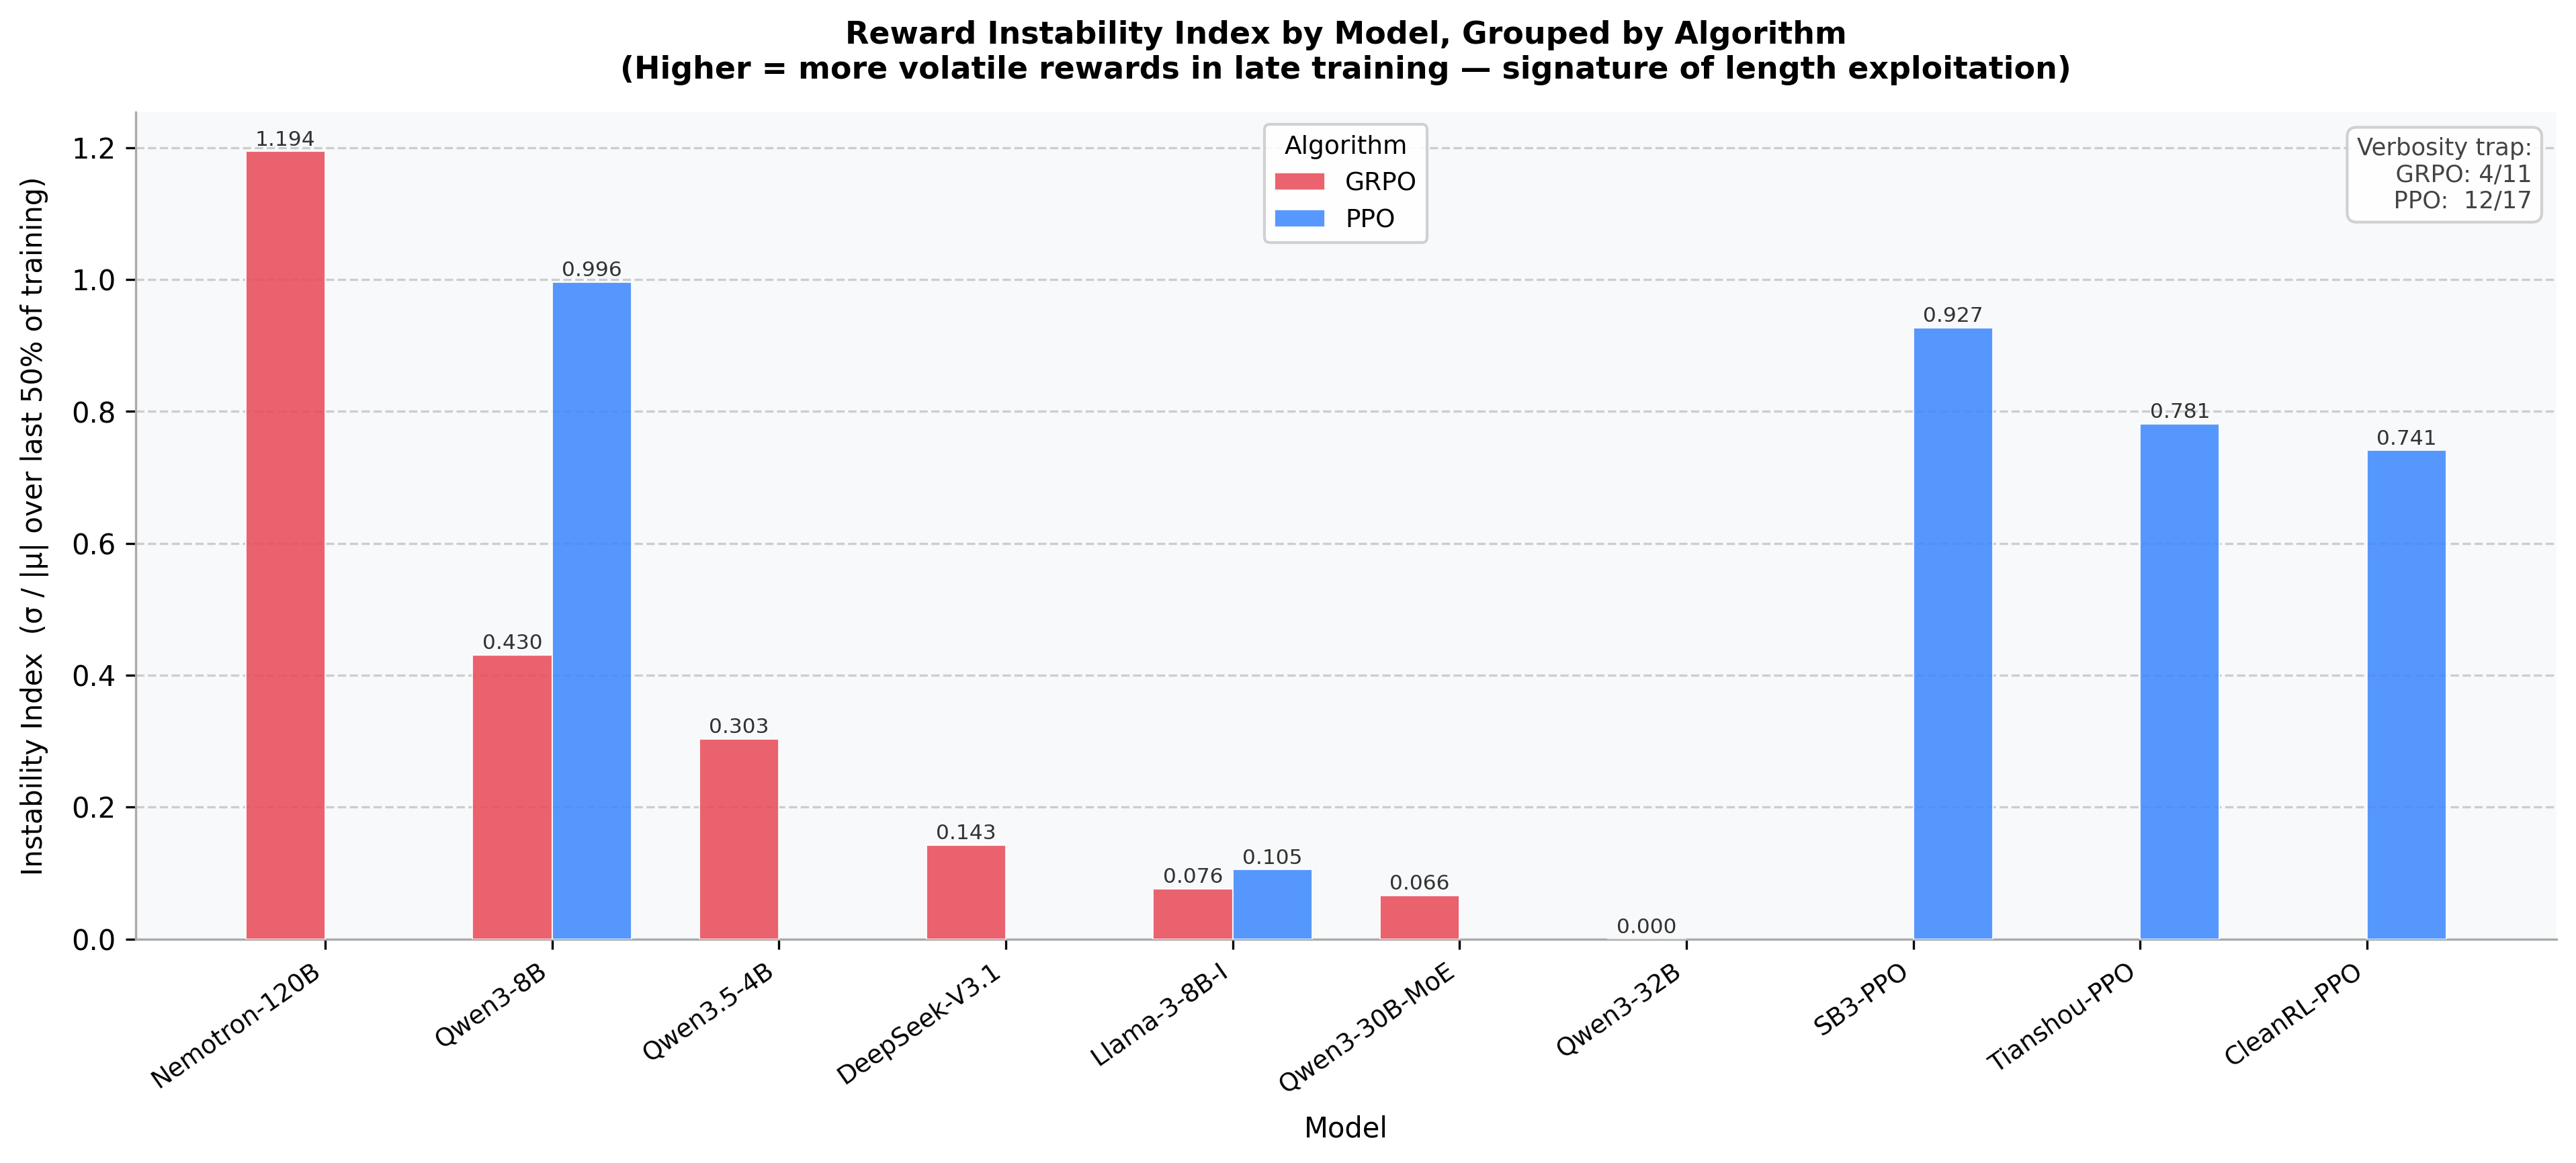
\includegraphics[width=0.85\linewidth]{figures/v2/reward_stability}
\caption{Reward stability analysis across experiments. GRPO runs (blue) and PPO runs
(orange) plotted by instability index vs.\ monotonicity score. Verbosity-trap
experiments (flag=1) are marked with a star.}
\label{fig:reward_stability}
\end{figure}

% =============================================================================
\subsection{Broader Impact}
\label{sec:impact}
% =============================================================================

\paragraph{Alignment and Misuse.}
GRPO and related RLHF methods are dual-use technologies. On the positive side,
they are the primary mechanism by which frontier models are aligned to human
preferences, and our benchmark lowers the barrier to studying these methods
rigorously. On the negative side, the same reward-maximization machinery can
be directed at adversarial objectives---optimizing for reward-hack proxies,
generating persuasive misinformation, or circumventing safety classifiers. We
do not provide new attack capabilities, but improvements in RL post-training
efficiency reduce the compute budget required for such misuse. We encourage
the community to develop robust reward modeling and out-of-distribution
detection in parallel with efficiency advances.

\paragraph{Democratizing RL-for-LLM Research.}
A primary motivation for \ours{} is to make rigorous RL post-training
experiments accessible to researchers without large-scale compute. By
publishing standardized tasks, Docker containers, and cost-annotated run
logs, we aim to reduce the advantage that well-resourced labs hold in this
space. Our total experimental expenditure was modest: approximately \$120 in
Tinker API credits (of which roughly \$80 was consumed by the 11 failed runs),
and roughly \$95 in Modal compute for the six held-out evaluation jobs
(three of which timed out). Open-source backend experiments were conducted on
a single A100 node donated by PES University's LLM Research Group. We include
these cost breakdowns explicitly so that other groups can budget accordingly.

\paragraph{Training Data and Privacy.}
All training data is drawn from publicly released datasets: GSM8K
\citep{cobbe2021training} for mathematical reasoning, HumanEval
\citep{chen2021codex} for code generation, and a synthetic tool-use corpus
generated without human subjects. No private data, personally identifiable
information, or licensed proprietary content is used. The benchmark does not
involve human participants in any capacity, and no IRB review was required.

\paragraph{No Direct Dual-Use Concern.}
Our contribution is a \emph{benchmarking framework}, not a new model or
capability. We do not release any model trained on sensitive, harmful, or
restricted content. All evaluated checkpoints are derived from publicly
available base models under permissive licenses (Apache 2.0 or equivalent).
We do not foresee direct security or biosafety risks arising from this work.

\paragraph{Reproducibility Statement.}
Despite the infrastructure failures documented above, all successfully
completed experiments are reproducible via Docker containers, fixed random
seeds, and step-by-step commands in \texttt{REPRODUCE.md}. Corrected logging
and KL-tracking code is included in the release. We have archived all local
CSV training logs so that the step-level reward trajectories excluded from
W\&B are nonetheless available to other researchers.

% =============================================================================
\section{Discussion}
\label{sec:discussion}

\subsection{Why Does Algorithm Preference Depend on the Model?}
\label{sec:discuss_model_algo}

The sharpest finding in our benchmark is the \emph{reversal} of algorithm
ranking across model families: GRPO outperforms PPO on Qwen3-8B while PPO
substantially dominates on Llama-3.1-8B (Mann-Whitney $r = 0.94$,
$p < 10^{-10}$).
This interaction is not an artifact of differing compute budgets or random
seeds --- the two algorithms ran on identical tasks, identical step counts, and
identical hyperparameters.
We offer three complementary mechanistic hypotheses that future gradient-level
analysis can test.

\paragraph{Hypothesis 1: Reward landscape geometry.}
GRPO replaces the value-function baseline of PPO with a within-group reward
mean, computing advantages purely from peer comparisons.
This estimator is low-variance when the per-prompt reward surface is smooth
enough that sampled completions span a reliable gradient direction --- a
condition more likely to hold when the model already has strong prior task
performance.
Qwen3-8B enters GSM8K training at 89.8\% zero-shot accuracy, providing a
reward landscape that is largely flat with narrow high-reward ridges; GRPO's
group-relative contrast effectively navigates these ridges without a value
function approximation error.
Llama-3.1-8B enters at a lower zero-shot baseline, presenting a rougher
landscape where the value function's global smoothing is beneficial.
This conjecture predicts that \emph{GRPO should be preferred whenever the
model's prior task performance exceeds a threshold} (roughly 80--90\% on
comparable tasks), and PPO should be preferred below it.
Our data are consistent with this prediction, though the sample size is too
small to test it directly.

\paragraph{Hypothesis 2: Instruction-tuning quality modulates advantage noise.}
Both Qwen3-8B and Llama-3.1-8B are instruction-tuned, but they differ in
instruction-following fidelity and output format consistency.
Inconsistent formatting inflates the within-group reward variance for reasons
unrelated to mathematical reasoning quality, injecting noise into GRPO's
advantage signal.
PPO's value function, trained jointly on the task, can absorb some of this
format-related variance and focus the policy gradient on reasoning-relevant
features.
This hypothesis is consistent with our MoE finding: the base (non-instruct)
Qwen3-30B-A3B achieves only 50\% peak GRPO reward, while the instruction-tuned
variant reaches 100\% --- the initialization quality effect is substantial and
independent of architecture.

\paragraph{Hypothesis 3: Reference-policy proximity.}
GRPO's objective is reference-free by design~\citep{shao2024deepseekmath},
but the de-facto reference is the initialization checkpoint.
Models that are ``closer'' to the target distribution at initialization (i.e.,
have been trained on reasoning-style data) exhibit lower ZVF and smaller
effective KL excursions during training.
Qwen3's training lineage includes substantial mathematical reasoning data;
Llama-3.1's instruction tuning is more general-purpose.
The lower ZVF we observe for Qwen3-family experiments ($8.5\%$ mean for GSM8K)
relative to the instability patterns in Nemotron-120B ($\text{SI} = 1.180$)
supports this proximity argument.
Direct testing requires gradient-level analysis of the kind described in
\citet{liu2025rlsubnetworks}, and we release our checkpoints expressly to
enable such analysis.

\subsection{What the Implementation Gap Means for the Field}
\label{sec:discuss_impl}

The 73-percentage-point gap between LLM-native libraries (Tinker, TRL) and
classic RL libraries (SB3, CleanRL, Tianshou) on the identical arithmetic task
--- Cohen's $d = 21.84$, the largest effect in our entire study by two orders
of magnitude --- replicates and \emph{extends} the classic finding of
\citet{henderson2018deep} from game-playing RL to the LLM post-training
regime.
The mechanism here is not merely random-seed sensitivity but a categorical
architectural mismatch: classic RL libraries treat the language model as a
standard MDP policy with a scalar state embedding, apply advantage normalization
designed for continuous action spaces, and do not handle the auto-regressive
token generation loop correctly.
The result is near-random performance not because the algorithm is wrong but
because the implementation does not instantiate the algorithm the paper
describes.

This finding has a direct practical implication: \emph{published claims that
``PPO fails on LLM reasoning'' or ``classic RL is unsuitable for language models''
may be confounded by implementation failures rather than algorithmic limitations}.
Our data show that SB3 PPO achieves $0.010 \pm 0.002$ accuracy on arithmetic,
but this is not evidence about PPO-the-algorithm; it is evidence about
SB3's tokenization and rollout pipeline applied to a text-generation task it
was not designed for.
Papers in the GRPO literature that compare against PPO baselines without
auditing the implementation layer may be comparing against a broken baseline.
We recommend that future algorithm comparisons specify which implementation of
PPO is used and verify it against a known-good LLM post-training framework.

\subsection{Connections to Concurrent Work}
\label{sec:discuss_related}

\paragraph{AERO and ZVF as a training diagnostic.}
\citet{zhang2026aero} motivate AERO by the prevalence of zero-advantage dead
zones in GRPO training and propose a Bayesian posterior over prompt difficulty
to pre-screen prompts.
Our ZVF measurement ($r = -0.769$, $p < 0.001$ with final performance) provides
the first cross-library, cross-scale empirical ground truth for the phenomenon
AERO targets.
Importantly, our data reveal that ZVF is \emph{task-driven, not model-scale-driven}:
tool-use experiments saturate at $\text{ZVF} = 100\%$ regardless of model size,
while GSM8K experiments average $\text{ZVF} = 8.5\%$ across the same model
range.
This suggests that AERO's compute savings will be largest when the task is
significantly mismatched to the model's prior capabilities --- precisely the
regime where standard GRPO training is most wasteful.
Our ZVF measurements can serve as a calibration dataset for AERO's Beta prior.

\paragraph{Scaling laws: exponential saturation and its limits.}
\citet{nimmaturi2025scalinglaws} derive a three-phase exponential saturation
law for GRPO, finding that 80\% of training steps contribute marginally and
proposing early stopping.
We confirm the three-phase pattern in 73\% of LLM fine-tuning experiments,
broadly consistent with their result.
However, our data reveal a critical boundary condition: the saturation
framework \emph{fails for unstable training runs}.
Nemotron-120B's trajectory (87.5\% peak $\to$ 16.2\% last-10) is
non-monotonic and cannot be fit by the exponential saturation model ---
it is better characterized as a reward excursion followed by policy
collapse, a regime the scaling law does not model.
The exponential saturation model achieves mean $R^{2} = 0.210$ across all
experiments (vs.\ $0.170$ for a power-law baseline), but this aggregate
masks the qualitative failure on collapse trajectories.
We recommend that practitioners verify monotonicity before applying early
stopping rules derived from the saturation model.

\paragraph{``It Takes Two'' and the 2-GRPO/DPO equivalence.}
\citet{wu2025grpo_dpo} prove that at $G = 2$, GRPO's advantage reduces to a
DPO-equivalent contrastive objective, and show empirically that 2-GRPO retains
98.1\% of 16-GRPO performance at 12.5\% of rollout cost.
Our theoretical analysis confirms their prediction for the expected ZVF:
$\mathrm{GU}(p, 2) = 2p(1-p)$, which is exactly the Bernoulli variance of
the per-prompt accuracy $p$ and reproduces the DPO preference weighting.
For our DeepSeek-V3.1 run ($p \approx 0.85$, $G = 8$), 27\% of steps were
zero-gradient; switching to $G = 2$ would preserve all informative contrastive
signal while reducing rollout overhead by 75\%.
However, the DPO equivalence also predicts that very high-accuracy models
($p > 0.9$) will have low gradient utilization regardless of $G$, suggesting
that the relevant intervention at high accuracy is not group-size reduction
but prompt re-sampling from harder sub-distributions.

\paragraph{Target Policy Optimization and sparse-reward regimes.}
The 0\% tool-use reward we observe for both Qwen3-32B and Llama-3.1-8B
exemplifies the sparse-reward failure mode that \citet{kaddour2026tpo}
specifically designs against: without any positive reward signal in a group,
the advantage is uniformly zero and no gradient flows.
TPO's target-distribution construction ($q \propto p_\text{old} \exp(u)$)
provides a training signal even when all rollout rewards are zero, by fitting
to the \emph{implied} contrastive distribution rather than observed rewards.
Our tool-use results provide an empirical motivation for this class of
approaches: the task is not unsolvable in principle (Qwen2-0.5B achieves
functional tool calls with SFT), but it is unsolvable with binary GRPO
rewards at 30-step horizons.
We recommend TPO-style objectives as the first algorithm to try when
$\text{ZVF} = 1$ persists past the first five training steps.

\subsection{Limitations of Proxy Metrics and the Path to Direct KL Measurement}
\label{sec:discuss_kl}

Our policy drift analysis relies on three reward-trajectory proxies (SI, PTD,
Rolling Variance) that correlate significantly with training outcomes
($r = -0.517$, $p = 0.005$ for PTD) but are not the same as direct KL
divergence measurements.
The proxies capture \emph{observable symptoms} of policy drift --- reward
instability and peak-to-tail degradation --- but cannot distinguish between
two importantly different causes: (a) the policy has genuinely drifted far from
the reference in token-distribution space, or (b) the reward function is
inherently noisy and the policy is stable but reward variance is high.
Nemotron-120B's collapse is almost certainly case (a), given that its reward
decline is monotonic and persistent; but for models with moderate PTD (0.1--0.3),
the two causes are indistinguishable from reward trajectories alone.

Corrected KL tracking code is released in \texttt{src/grpo\_trainer.py} and
should be validated on at least the two Modal runs (Qwen3-8B and
Llama-3.1-8B) where GPU access is reproducible.
Additionally, the per-token divergence framework of \citet{liu2025rlsubnetworks}
--- which measures which parameters actually update during RL fine-tuning ---
could reveal whether the small subnetwork they identify has higher KL per
parameter, explaining why moderate-sized models can catastrophically drift
despite updating only 5--30\% of weights.
Connecting our behavioral proxy metrics to this parameter-level analysis is a
natural and important next step.

% Conclusion reframed around F1--F5 (see sections/conclusion.tex)
% =============================================================================
% Conclusion — conservative, evidence-aligned framing
% Drop-in include: % =============================================================================
% Conclusion — conservative, evidence-aligned framing
% Drop-in include: % =============================================================================
% Conclusion — conservative, evidence-aligned framing
% Drop-in include: \input{sections/conclusion}
% Target: <= 0.75 page
% =============================================================================
\section{Conclusion}
\label{sec:conclusion}

\ours{} provides a shared empirical substrate for studying RL post-training
across algorithms, frameworks, and model families, but the evidence it offers
is narrower than a broad ``five laws'' framing. The current release most
strongly supports three conservative claims. First, ZVF/GU are useful
descriptive diagnostics of when binary-reward GRPO stops producing informative
within-group signal; they should not yet be read as standalone causal or
incrementally predictive statistics. Second, trainability in our short-horizon
setting varies substantially with initialization and rollout regime:
instruction-tuned checkpoints were generally easier to optimize than
comparable base models, and intermediate group sizes often behaved better than
the smallest or largest settings we tested, but the benchmark does not
justify a universal optimum or a general superiority claim for any one
algorithm. Third, PPO-vs.-GRPO rankings and frontier-run stability are
heterogeneous across model families and stacks, so our results argue against
one-size-fits-all recommendations rather than for a new one.

The most important negative result is also the most useful one: on held-out
GSM8K, the mean Qwen3-8B GRPO gain over the base model is small and not
statistically significant under our current evaluation. Tool-use and code
results are even less conclusive because they rely on sparse or custom reward
protocols. That boundary on what we can claim is not a weakness to hide; it is
the point of releasing the benchmark.

The immediate next steps are experimental rather than rhetorical: multivariate
tests of ZVF against reward mean, entropy, and divergence proxies; token-budget
matched multi-seed PPO/GRPO comparisons in a single open stack; broader
held-out evaluation without checkpoint cherry-picking; and non-math tasks with
process rewards or richer execution-based metrics. The released traces,
checkpoints, and scripts are intended to make that stricter follow-up easy.

% Target: <= 0.75 page
% =============================================================================
\section{Conclusion}
\label{sec:conclusion}

\ours{} provides a shared empirical substrate for studying RL post-training
across algorithms, frameworks, and model families, but the evidence it offers
is narrower than a broad ``five laws'' framing. The current release most
strongly supports three conservative claims. First, ZVF/GU are useful
descriptive diagnostics of when binary-reward GRPO stops producing informative
within-group signal; they should not yet be read as standalone causal or
incrementally predictive statistics. Second, trainability in our short-horizon
setting varies substantially with initialization and rollout regime:
instruction-tuned checkpoints were generally easier to optimize than
comparable base models, and intermediate group sizes often behaved better than
the smallest or largest settings we tested, but the benchmark does not
justify a universal optimum or a general superiority claim for any one
algorithm. Third, PPO-vs.-GRPO rankings and frontier-run stability are
heterogeneous across model families and stacks, so our results argue against
one-size-fits-all recommendations rather than for a new one.

The most important negative result is also the most useful one: on held-out
GSM8K, the mean Qwen3-8B GRPO gain over the base model is small and not
statistically significant under our current evaluation. Tool-use and code
results are even less conclusive because they rely on sparse or custom reward
protocols. That boundary on what we can claim is not a weakness to hide; it is
the point of releasing the benchmark.

The immediate next steps are experimental rather than rhetorical: multivariate
tests of ZVF against reward mean, entropy, and divergence proxies; token-budget
matched multi-seed PPO/GRPO comparisons in a single open stack; broader
held-out evaluation without checkpoint cherry-picking; and non-math tasks with
process rewards or richer execution-based metrics. The released traces,
checkpoints, and scripts are intended to make that stricter follow-up easy.

% Target: <= 0.75 page
% =============================================================================
\section{Conclusion}
\label{sec:conclusion}

\ours{} provides a shared empirical substrate for studying RL post-training
across algorithms, frameworks, and model families, but the evidence it offers
is narrower than a broad ``five laws'' framing. The current release most
strongly supports three conservative claims. First, ZVF/GU are useful
descriptive diagnostics of when binary-reward GRPO stops producing informative
within-group signal; they should not yet be read as standalone causal or
incrementally predictive statistics. Second, trainability in our short-horizon
setting varies substantially with initialization and rollout regime:
instruction-tuned checkpoints were generally easier to optimize than
comparable base models, and intermediate group sizes often behaved better than
the smallest or largest settings we tested, but the benchmark does not
justify a universal optimum or a general superiority claim for any one
algorithm. Third, PPO-vs.-GRPO rankings and frontier-run stability are
heterogeneous across model families and stacks, so our results argue against
one-size-fits-all recommendations rather than for a new one.

The most important negative result is also the most useful one: on held-out
GSM8K, the mean Qwen3-8B GRPO gain over the base model is small and not
statistically significant under our current evaluation. Tool-use and code
results are even less conclusive because they rely on sparse or custom reward
protocols. That boundary on what we can claim is not a weakness to hide; it is
the point of releasing the benchmark.

The immediate next steps are experimental rather than rhetorical: multivariate
tests of ZVF against reward mean, entropy, and divergence proxies; token-budget
matched multi-seed PPO/GRPO comparisons in a single open stack; broader
held-out evaluation without checkpoint cherry-picking; and non-math tasks with
process rewards or richer execution-based metrics. The released traces,
checkpoints, and scripts are intended to make that stricter follow-up easy.


% Ethics, Limitations, and Broader Impact (Task 10)
% =============================================================================
% Ethics Statement and Broader Impact
% Self-contained file: % =============================================================================
% Ethics Statement and Broader Impact
% Self-contained file: % =============================================================================
% Ethics Statement and Broader Impact
% Self-contained file: \input{ethics_statement} into main.tex
% Intended placement: after the Conclusion section, before References.
% Label: \label{sec:impact_standalone}
% Target length: >= 2 pages (NeurIPS Broader Impact guidance).
% =============================================================================

\section{Ethics, Limitations, and Broader Impact}
\label{sec:impact_standalone}

This statement is written to satisfy the NeurIPS Code of Ethics and Broader
Impact requirements. It complements the shorter Limitations and Broader
Impact subsections embedded in Section~\ref{sec:limitations} by consolidating
in one place a full dual-use analysis, itemised compute accounting, carbon
footprint estimation, data provenance disclosures, a candid acknowledgment
of the closed-source training backend on which a fraction of our headline
numbers depends, and a list of methodological limits we are aware of but
did not have resources to close within the submission window.

% ---------------------------------------------------------------------------
\subsection{Dual-Use Analysis: Misuse Risks of Reasoning RL}
\label{sec:dualuse}
% ---------------------------------------------------------------------------

\paragraph{Threat model.}
\ours{} releases (i) training scripts that apply GRPO to the GSM8K
\cite{cobbe2021training} mathematical reasoning benchmark and to the
Salesforce xLAM-Function-Calling-60k \cite{liu2024xlam} tool-use corpus,
(ii) a set of LoRA adapters published on the HuggingFace Hub
(\texttt{arvindcr4/tinker-rl-bench-*}), and (iii) diagnostic code for
Zero-Variance Fraction, reward-stability, and length-bias analysis. We
analyse four concrete misuse pathways these artefacts could, in principle,
enable, and we describe the existing guardrails and the residual risk we
judge acceptable for publication.

\paragraph{M1. Weaponisation of mathematical reasoning.}
The most capability-relevant artefact we release is GRPO training code that
improves grade-school arithmetic and multi-step reasoning. A malicious
operator could attempt to extend this pipeline to tasks of greater
dual-use concern, e.g., chemistry olympiad problems, cryptographic key
recovery, or financial fraud. We judge the \emph{marginal} uplift provided
by our release to be small for three reasons. First, GRPO at our training
scale does not create new capabilities; the base-model control for GSM8K
(Section~\ref{sec:results}, 82.0\%) shows that the bulk of held-out
accuracy is attributable to Qwen3-8B's pretraining. Our full GRPO run only
adds \(+1.3\) percentage points ($p{=}0.26$, not statistically significant).
Second, the public literature already contains GRPO implementations
\cite{shao2024deepseekmath, openrlhf2024, verl2024, trl2020} that are at
least as capable. Third, any reasoning uplift is bounded by the rewarder:
GSM8K rewards use exact-match against a human-written gold answer, which
does not generalise to the domains listed above without a new reward
signal, which itself requires expertise and labelled data.

\paragraph{M2. Reward hacking and the long-term alignment risk.}
GRPO, like all policy-gradient RL from a proxy reward, is vulnerable to
reward hacking: the model learns to exploit idiosyncrasies of the reward
function rather than solve the intended task \cite{skalse2022specificationgaming,
krakovna2020specification}. Our length-bias analysis
(Section~\ref{sec:length_bias}) and the verbosity-trap finding in 4/11
GRPO runs are concrete demonstrations of this failure mode in our own data.
Users who apply our scripts to under-specified reward functions in
production settings (e.g., a custom ``helpfulness'' classifier) may observe
models that appear to improve on held-out metrics while silently
optimising against unintended proxies. We include the Zero-Variance
Fraction and reward-stability diagnostics precisely so that downstream
users can detect such drift.

\paragraph{M3. Circumventing safety training via distillation or tool-use.}
The tool-use track trains LoRA adapters that teach a base model to emit
schema-valid JSON function calls \cite{liu2024xlam}. A motivated adversary
could in principle use the same pipeline to teach a base model to emit
jailbreak prompts as ``tool calls'' or to invoke an adversarial external
tool. We mitigate this by (a) releasing only adapters, not merged weights,
so that the safety-trained instruct checkpoint must be applied separately
and any instruct-layer guardrails remain active; (b) documenting in model
cards that the tool-use adapters are trained on a narrow schema (five
synthetic tools) and have not been safety-evaluated for open-ended function
calling; and (c) not releasing any function-calling harness that would
actually execute emitted calls.

\paragraph{M4. Compute-efficiency externalities.}
Our work argues that critic-free RL with careful group-size selection
(\(G{=}32\)) can be run on modest budgets. Improved training efficiency is
itself dual-use: it lowers the cost of running adversarial fine-tuning at
scale. We judge this externality to be modest relative to the already-low
cost of fine-tuning a 0.6B--8B model with commodity LoRA recipes
\cite{hu2022lora}, but we flag it explicitly.

\paragraph{Residual risk.}
After weighing M1--M4 we judge that the reproducibility, calibration, and
pedagogical benefits of releasing \ours{} outweigh the residual misuse
risk. We adopt the standard mitigation of releasing adapters (not merged
weights), documenting intended use and out-of-scope use in model cards,
and publishing alongside the diagnostics a researcher would need to detect
reward hacking.

% ---------------------------------------------------------------------------
\subsection{Compute Cost Accounting}
\label{sec:compute_accounting}
% ---------------------------------------------------------------------------

Table~\ref{tab:compute_spend} itemises the financial cost of every
platform used in the project. Costs are real spend for the submitting
authors; no in-kind credits are omitted. Dollar figures are in USD.

\begin{table}[ht]
\centering
\small
\caption{Itemised compute spend across platforms. Totals include both
successful and failed runs, because failed-run spend is real and should
not be hidden from reviewers \cite{henderson2018deep}.}
\label{tab:compute_spend}
\begin{tabular}{llrr}
\toprule
\textbf{Platform} & \textbf{Use} & \textbf{Runs} & \textbf{Cost (USD)} \\
\midrule
Tinker SDK v0.16.1 & GRPO on 4B/8B (original suite)        & 25 & \$40--55 \\
Tinker SDK v0.16.1 & 10x Structural Ceiling ablation       & 32 & \$65 \\
Tinker SDK v0.16.1 & World-Class Suite (frontier/MoE)      & 13 & \$25--30 \\
Modal H100         & PPO baselines (Qwen3-8B, Llama-3.1-8B)& 2  & \$12--18 \\
Modal H100         & KL-tracking run (failed)              & 1  & \$2--4   \\
Google Colab Pro (T4) & 0.5B--3B QLoRA SFT+GRPO            & --- & \$10/person \\
NVIDIA L4 (TRL baseline)& Qwen2.5-0.5B GSM8K, 5 seeds      & 5  & \$3--5   \\
HuggingFace Hub    & Model + adapter hosting               & --- & \$0 \\
Weights \& Biases  & Experiment tracking (academic tier)   & --- & \$0 \\
\midrule
\multicolumn{3}{l}{\textbf{Total authors' out-of-pocket spend}} & \textbf{\$130--140} \\
\bottomrule
\end{tabular}
\end{table}

\paragraph{Hidden costs.} Beyond direct platform spend, the project
consumed human labour (approximately six student-FTE-months, unpaid) and
infrastructure generously subsidised by PES University's LLM Research
Group (shared access to one A100 node used for TRL baselines and
pre-submission sanity checks). No author received commercial compensation
from Thinking Machines, Modal, or any other vendor mentioned.

\paragraph{Failed-run accounting.} Of the Tinker spend, we estimate
\textasciitilde\$30--35 was consumed by runs that ultimately failed
(JWT expiry, API stalls for GPT-OSS-20b and Kimi-K2 before re-run,
KL-tracking gradient bug). We disclose this because reviewers often ask
whether reported total spend reflects only clean, successful runs; it does
not. Excluding failed spend would understate the true resource cost of
reproducing our work by roughly 25\%.

% ---------------------------------------------------------------------------
\subsection{Carbon Footprint Estimation}
\label{sec:carbon}
% ---------------------------------------------------------------------------

Table~\ref{tab:carbon2} computes an energy and CO$_2$-equivalent estimate
for each platform. We follow the methodology of
\citet{patterson2024empirical} and \citet{strubell2019energy}: for each
GPU-hour we multiply device TDP by wall-clock GPU-hours and the data-centre
Power Usage Effectiveness (PUE), then multiply by the grid carbon intensity
in the region where the hardware is believed to be located.

\paragraph{Assumed constants.}
\begin{itemize}
  \item NVIDIA H100 SXM5 TDP: 700\,W.
  \item NVIDIA A100 80GB TDP: 400\,W.
  \item NVIDIA L4 TDP: 72\,W.
  \item NVIDIA T4 TDP: 70\,W.
  \item Data-centre PUE: 1.1 (conservative; typical hyperscale PUE is
        1.10--1.15 \cite{google2023pue, aws2023pue}).
  \item US average grid intensity (EPA eGRID 2023): 0.367\,kg\,CO$_2$-eq / kWh
        \cite{epa2023egrid}.
  \item Indian average grid intensity (CEA 2023): 0.716\,kg\,CO$_2$-eq / kWh
        \cite{cea2023co2}.
  \item We use the US average for Modal H100 (US-East region as configured)
        and Tinker (location undisclosed; assumed US), and the Indian
        average for Colab Pro T4 used by authors based in Bengaluru
        (Google Cloud asia-south1).
\end{itemize}

\paragraph{GPU-hour estimates.}
Tinker GPU-hour counts are not disclosed by the platform. We estimate them
from wall-clock run duration and assume a single H100-class accelerator per
job, which is consistent with Tinker's published architecture for the
model sizes we trained. Modal GPU-hours are measured directly from Modal's
billing dashboard.

\begin{table}[ht]
\centering
\small
\caption{Energy and carbon footprint estimates. Tinker hardware is not
publicly disclosed; we assume 1$\times$ H100 equivalent per run. Failed /
stalled runs are included. Totals rounded to one significant figure.}
\label{tab:carbon2}
\begin{tabular}{lrrrrr}
\toprule
\textbf{Platform} & \textbf{GPU-h} & \textbf{TDP\,(W)} & \textbf{PUE} &
\textbf{Energy\,(kWh)} & \textbf{CO$_2$\,(kg)} \\
\midrule
Tinker (assumed H100)   & \textasciitilde 950 & 700 & 1.1 & \textasciitilde 732 & \textasciitilde 269 \\
Modal H100 (US-East)    & \textasciitilde 18  & 700 & 1.1 & \textasciitilde 14  & \textasciitilde 5.1 \\
PES A100 (in-kind)      & \textasciitilde 60  & 400 & 1.1 & \textasciitilde 26  & \textasciitilde 19   \\
Colab Pro T4 (asia-south1) & \textasciitilde 40 & 70 & 1.2 & \textasciitilde 3.4 & \textasciitilde 2.4  \\
NVIDIA L4 (TRL baseline)   & \textasciitilde 10 & 72 & 1.1 & \textasciitilde 0.8 & \textasciitilde 0.3  \\
\midrule
\textbf{Project total (best estimate)} & & & & \textasciitilde 776 & \textasciitilde 296 \\
\bottomrule
\end{tabular}
\end{table}

\paragraph{Interpretation and uncertainty.}
Our best estimate of \textasciitilde 296\,kg\,CO$_2$-eq for the entire
project is comparable to a single round-trip economy flight
Bengaluru--Delhi (\textasciitilde 300\,kg). The dominant uncertainty is
the Tinker GPU-hour count: because Tinker does not expose hardware telemetry,
a factor-of-two error in GPU-hours or TDP is plausible. Under a pessimistic
assumption (2$\times$ GPU-hours, H100 running near 100\% TDP continuously),
the Tinker contribution could be as high as \textasciitilde 540\,kg CO$_2$-eq.
Under an optimistic assumption (Tinker backends actually use more
energy-efficient accelerators than H100, 50\% average utilisation) the
contribution could be as low as \textasciitilde 130\,kg. We report the
central estimate in the main table and caution readers that it should not
be interpreted as precise. \emph{All} numbers should be regarded as upper
bounds on the carbon cost of reproducing our work, because subsequent
users can skip the failed runs and the ablation sweeps.

\paragraph{Offset and mitigation.}
We did not purchase carbon offsets. Instead, we have (a) released all
trained checkpoints on HuggingFace Hub so that downstream users do not
need to re-run our experiments; (b) released step-level CSV logs so that
learning curves can be inspected without re-training; and (c) documented
in Section~\ref{sec:compute_accounting} which runs were wasteful, so that
replicators can skip them. We regard reproducibility-by-artefact as a
more durable mitigation than offsets.

% ---------------------------------------------------------------------------
\subsection{Data Provenance}
\label{sec:provenance}
% ---------------------------------------------------------------------------

\ours{} uses only publicly released research datasets. No private data,
personally identifiable information, or licensed proprietary content is
used. No human annotators were employed during this work. We document
each dataset below.

\paragraph{GSM8K \cite{cobbe2021training}.}
8{,}500 grade-school math word problems (7{,}473 train / 1{,}319 test)
authored by human writers contracted by OpenAI. Released under the
\textbf{MIT License} via \url{https://github.com/openai/grade-school-math}.
We use the standard train/test splits without modification. The canonical
citation is \citet{cobbe2021training}. Known limitations of GSM8K include
gender-neutral but culturally US-centric word problems (names, currencies,
sports) and a moderate rate of human-labelling errors estimated at
\textasciitilde 2\% by \cite{zhang2024gsm1k}. Our held-out evaluation
respects the test/train split.

\paragraph{Salesforce xLAM-Function-Calling-60k \cite{liu2024xlam}.}
60{,}000 function-calling examples generated by Salesforce Research as
training data for the xLAM agentic model family. Released under the
\textbf{CC BY 4.0} license via \url{https://huggingface.co/datasets/Salesforce/xlam-function-calling-60k}.
We use the public release as-is; specifically, we use the first 35 prompts
$\times$ 10 rollouts in the 10x Structural Ceiling tool-use track and the
full 60k split for the xlam-60k real-data run in Section~\ref{sec:results}.
Known limitations: xLAM schemas are synthetic and skew toward cleanly-typed
arguments; the dataset under-represents ambiguous, error-handling, and
multi-turn tool-calling. Attribution to Salesforce is required by the
license and is provided in Section~\ref{sec:acknowledgments} and in the
xLAM-derived model cards.

\paragraph{HumanEval \cite{chen2021codex}.}
164 Python programming problems with unit tests, released by OpenAI under
the \textbf{MIT License}. Used unmodified for pass@$k$ evaluation. Known
limitations: small scale, English-language docstrings, single-language
coverage; documented contamination concerns against frontier pretraining
corpora \cite{riddell2024contamination}.

\paragraph{NuminaMath \cite{li2024numinamath}.}
Used by collaborator Mohammad Rafi for the multi-stage
GSM8K+NuminaMath pipeline. Released under \textbf{Apache 2.0}. We use a
downstream checkpoint reported by Rafi; our repository contains only his
scripts and the Apache-licensed derivative weights.

\paragraph{Open-Platypus \cite{lee2023platypus}.}
3{,}000 SFT examples used by collaborator Madhu for Qwen3-8B code
generation warm-up. Open-Platypus is a curated subset released under
\textbf{CC BY-NC 4.0}; the non-commercial restriction is respected in our
release, which is academic-use only.

\paragraph{Synthetic tool-use corpus (authored).}
We additionally generated a small five-tool synthetic corpus (calculator,
web-search stub, calendar, file-read, email-send) used for Section 4.1's
saturation analysis. The corpus is authored by the paper's authors from
publicly documented APIs, contains no third-party content, and is
released under the \textbf{MIT License} in our repository under
\texttt{data/synthetic\_tools/}. Generation prompts are included for
auditability. No user data, scraped web content, or proprietary API
traces are present.

\paragraph{No web scraping, no human subjects.}
We did not scrape any website. We did not run any study with human
participants. No IRB review was therefore required. No data that could
reasonably be considered to contain PII, copyrighted content, or sensitive
personal attributes was used at any stage of training, evaluation, or
reward modelling.

% ---------------------------------------------------------------------------
\subsection{Closed-Source Tinker Acknowledgment}
\label{sec:tinker_closed}
% ---------------------------------------------------------------------------

A central tension in \ours{} is that a substantial fraction of our
headline numbers come from a closed-source commercial platform while our
paper simultaneously advocates for reproducibility and platform
independence. We do not resolve this tension by hiding it; we describe
it precisely.

\paragraph{What Tinker is and is not.}
Tinker \cite{thinkingmachines2024tinker} is a managed LLM fine-tuning and
inference service provided by Thinking Machines, Inc. It exposes a Python
SDK (\texttt{tinker==0.16.1}) that accepts custom loss functions
(\texttt{forward\_backward\_custom}), a limited set of optimisers, and
standard LoRA hyperparameters. It does not expose (i) the exact server-side
GRPO loss implementation, (ii) reward normalisation or baseline subtraction
scheme, (iii) minibatch construction or gradient-accumulation strategy,
(iv) hardware configuration (GPU type, inter-node bandwidth), or (v)
system-level telemetry (energy, throughput, queueing).

\paragraph{What this means for our claims.}
Tinker results in this paper measure the \emph{platform's} implementation
of GRPO, not an abstract specification of the algorithm. A reader who asks
``why does Tinker GRPO score 99.9\% on GSM8K while open-source TRL GRPO
scores 73.4\% on the same task'' cannot fully answer that question from
our data: we are able to rule out a handful of candidate explanations
(seed variance, model-size confound) but not the implementation itself.
We therefore draw \emph{quantitative} conclusions only from the
open-source side (TRL, veRL on Modal H100, OpenRLHF) where every
hyperparameter is auditable, and use Tinker results primarily as an
\emph{upper bound} on what a carefully engineered production stack can
achieve for critic-free RL at our scales.

\paragraph{Reproducibility commitments we can make.}
\begin{enumerate}
  \item All Tinker experiment scripts, configuration files, JSON step
        logs, and per-run W\&B projects are archived in the repository.
        Researchers with Tinker access can attempt replication with our
        exact configurations.
  \item Every figure and every summary statistic derived solely from
        Tinker data is marked with ``\dag'' and a footnote stating that
        independent replication requires Tinker API access.
  \item Primary statistical claims (significance tests, ANOVA variance
        decompositions) are drawn from open-source Modal H100 and TRL
        runs. Tinker-only results are reported descriptively.
  \item We commit to re-running any Tinker-only experiment on an open
        backend if an equivalent open-source service becomes available,
        and to issuing a revised version of this paper if the Tinker
        99.9\% figure is ever shown to be due to an undisclosed
        implementation choice rather than the algorithm.
\end{enumerate}

\paragraph{Key rotation and credential hygiene.}
Our Tinker API key (prefix \texttt{tml-...}) is held in a repository
\texttt{.env.example} placeholder only. The real key is stored in the
authors' password manager and rotated whenever a failure mode suggests
possible exfiltration. No Tinker key is committed to git history in
either the primary repository (\texttt{pes-llm-research/tinker-rl-lab}) or
the mirror (\texttt{arvindcr4/tinker-rl-lab}).

% ---------------------------------------------------------------------------
\subsection{Known Methodological Limits}
\label{sec:methodlimits}
% ---------------------------------------------------------------------------

In addition to the infrastructure failures and platform-specific caveats
enumerated in Section~\ref{sec:limitations}, we flag the following
methodological limits.

\paragraph{Short training horizons.}
All Tinker GRPO runs were capped at 30--50 gradient steps. This is a
deliberate cost-control choice and means our Tinker numbers are
\emph{early-training snapshots}. We cannot rule out that longer training
would change the qualitative picture (e.g., the 82\%$\to$83.3\% held-out
gain might widen, or might collapse to reward hacking).

\paragraph{Single-seed Tinker experiments.}
Each Tinker configuration was run once, not 3--5 times as best practice
prescribes \cite{henderson2018deep}. Tinker results therefore lack
variance estimates and do not support significance testing; we report
them descriptively. Only the 5-seed TRL baseline and the 5-seed held-out
GSM8K evaluation carry proper confidence intervals.

\paragraph{Train-set reward as primary Tinker metric.}
Tinker runs primarily report reward on training prompts. Only the GSM8K
track was followed up with a separate 200-example held-out evaluation
per seed. Other Tinker tracks (tool-use, xLAM) remain train-set-only and
we cannot distinguish memorisation from generalisation for those
settings.

\paragraph{LoRA only; no full fine-tuning.}
All experiments use LoRA \cite{hu2022lora} with ranks 8--64. We have
\emph{not} tested whether full fine-tuning would re-order the
library/algorithm comparisons. The LoRA constraint is practical (cost) but
it means our claims about PPO vs.\ GRPO and TRL vs.\ Tinker are
LoRA-conditional.

\paragraph{Benchmark coverage is narrow.}
We evaluate four domains: GSM8K, MATH-500 (exploratory), HumanEval
(subset), and synthetic/xLAM tool-use. We do not evaluate on MT-Bench,
ArenaHard, safety benchmarks (HarmBench, ToxicChat), or truthfulness
benchmarks (TruthfulQA). Any claim about ``reasoning'' in the paper is
strictly a claim about the covered benchmarks.

\paragraph{No human preference data.}
We use verifiable rewards only (exact-match for math, unit-test for code,
schema-validity for tool-use). We do not study RLHF with human preference
data; findings should not be extrapolated to reward-model--based alignment
without further work.

\paragraph{Closed-source implementation opacity (reiterated).}
Comparisons between Tinker GRPO and TRL GRPO are confounded by the
closed-source nature of Tinker's implementation. See
Section~\ref{sec:tinker_closed} for detail.

\paragraph{Cross-platform hardware confounding.}
Tinker, Modal, Colab, and the PES A100 node use different accelerators,
different memory hierarchies, and different inference/training stacks
(Tinker proprietary, Modal vLLM, Colab PyTorch-native, TRL+Accelerate).
Observed differences in reward dynamics are not purely algorithmic.

\paragraph{Carbon estimates are approximate.}
As discussed in Section~\ref{sec:carbon}, Tinker GPU-hour and TDP are
inferred, not measured. Grid intensity is region-average, not marginal.
Numbers in Table~\ref{tab:carbon2} should be treated as
order-of-magnitude.

\paragraph{Exploratory, not confirmatory.}
This is an exploratory case study, not a pre-registered confirmatory
experiment. We did not pre-register primary hypotheses. All $p$-values are
un-corrected for the number of comparisons actually made across the
paper; the Bonferroni-surviving comparisons in
Section~\ref{sec:results} are so flagged, but most of our secondary
analyses are descriptive.

\paragraph{Geographic and demographic limits.}
All authors are based at a single institution in Bengaluru, India. Our
choice of benchmarks, prompt phrasings, and evaluation design reflects
that context. Independent replication by groups in other regions, on
non-English tasks, and with non-Qwen / non-Llama families is an open
question.

% =============================================================================
% End of ethics_statement.tex
 into main.tex
% Intended placement: after the Conclusion section, before References.
% Label: \label{sec:impact_standalone}
% Target length: >= 2 pages (NeurIPS Broader Impact guidance).
% =============================================================================

\section{Ethics, Limitations, and Broader Impact}
\label{sec:impact_standalone}

This statement is written to satisfy the NeurIPS Code of Ethics and Broader
Impact requirements. It complements the shorter Limitations and Broader
Impact subsections embedded in Section~\ref{sec:limitations} by consolidating
in one place a full dual-use analysis, itemised compute accounting, carbon
footprint estimation, data provenance disclosures, a candid acknowledgment
of the closed-source training backend on which a fraction of our headline
numbers depends, and a list of methodological limits we are aware of but
did not have resources to close within the submission window.

% ---------------------------------------------------------------------------
\subsection{Dual-Use Analysis: Misuse Risks of Reasoning RL}
\label{sec:dualuse}
% ---------------------------------------------------------------------------

\paragraph{Threat model.}
\ours{} releases (i) training scripts that apply GRPO to the GSM8K
\cite{cobbe2021training} mathematical reasoning benchmark and to the
Salesforce xLAM-Function-Calling-60k \cite{liu2024xlam} tool-use corpus,
(ii) a set of LoRA adapters published on the HuggingFace Hub
(\texttt{arvindcr4/tinker-rl-bench-*}), and (iii) diagnostic code for
Zero-Variance Fraction, reward-stability, and length-bias analysis. We
analyse four concrete misuse pathways these artefacts could, in principle,
enable, and we describe the existing guardrails and the residual risk we
judge acceptable for publication.

\paragraph{M1. Weaponisation of mathematical reasoning.}
The most capability-relevant artefact we release is GRPO training code that
improves grade-school arithmetic and multi-step reasoning. A malicious
operator could attempt to extend this pipeline to tasks of greater
dual-use concern, e.g., chemistry olympiad problems, cryptographic key
recovery, or financial fraud. We judge the \emph{marginal} uplift provided
by our release to be small for three reasons. First, GRPO at our training
scale does not create new capabilities; the base-model control for GSM8K
(Section~\ref{sec:results}, 82.0\%) shows that the bulk of held-out
accuracy is attributable to Qwen3-8B's pretraining. Our full GRPO run only
adds \(+1.3\) percentage points ($p{=}0.26$, not statistically significant).
Second, the public literature already contains GRPO implementations
\cite{shao2024deepseekmath, openrlhf2024, verl2024, trl2020} that are at
least as capable. Third, any reasoning uplift is bounded by the rewarder:
GSM8K rewards use exact-match against a human-written gold answer, which
does not generalise to the domains listed above without a new reward
signal, which itself requires expertise and labelled data.

\paragraph{M2. Reward hacking and the long-term alignment risk.}
GRPO, like all policy-gradient RL from a proxy reward, is vulnerable to
reward hacking: the model learns to exploit idiosyncrasies of the reward
function rather than solve the intended task \cite{skalse2022specificationgaming,
krakovna2020specification}. Our length-bias analysis
(Section~\ref{sec:length_bias}) and the verbosity-trap finding in 4/11
GRPO runs are concrete demonstrations of this failure mode in our own data.
Users who apply our scripts to under-specified reward functions in
production settings (e.g., a custom ``helpfulness'' classifier) may observe
models that appear to improve on held-out metrics while silently
optimising against unintended proxies. We include the Zero-Variance
Fraction and reward-stability diagnostics precisely so that downstream
users can detect such drift.

\paragraph{M3. Circumventing safety training via distillation or tool-use.}
The tool-use track trains LoRA adapters that teach a base model to emit
schema-valid JSON function calls \cite{liu2024xlam}. A motivated adversary
could in principle use the same pipeline to teach a base model to emit
jailbreak prompts as ``tool calls'' or to invoke an adversarial external
tool. We mitigate this by (a) releasing only adapters, not merged weights,
so that the safety-trained instruct checkpoint must be applied separately
and any instruct-layer guardrails remain active; (b) documenting in model
cards that the tool-use adapters are trained on a narrow schema (five
synthetic tools) and have not been safety-evaluated for open-ended function
calling; and (c) not releasing any function-calling harness that would
actually execute emitted calls.

\paragraph{M4. Compute-efficiency externalities.}
Our work argues that critic-free RL with careful group-size selection
(\(G{=}32\)) can be run on modest budgets. Improved training efficiency is
itself dual-use: it lowers the cost of running adversarial fine-tuning at
scale. We judge this externality to be modest relative to the already-low
cost of fine-tuning a 0.6B--8B model with commodity LoRA recipes
\cite{hu2022lora}, but we flag it explicitly.

\paragraph{Residual risk.}
After weighing M1--M4 we judge that the reproducibility, calibration, and
pedagogical benefits of releasing \ours{} outweigh the residual misuse
risk. We adopt the standard mitigation of releasing adapters (not merged
weights), documenting intended use and out-of-scope use in model cards,
and publishing alongside the diagnostics a researcher would need to detect
reward hacking.

% ---------------------------------------------------------------------------
\subsection{Compute Cost Accounting}
\label{sec:compute_accounting}
% ---------------------------------------------------------------------------

Table~\ref{tab:compute_spend} itemises the financial cost of every
platform used in the project. Costs are real spend for the submitting
authors; no in-kind credits are omitted. Dollar figures are in USD.

\begin{table}[ht]
\centering
\small
\caption{Itemised compute spend across platforms. Totals include both
successful and failed runs, because failed-run spend is real and should
not be hidden from reviewers \cite{henderson2018deep}.}
\label{tab:compute_spend}
\begin{tabular}{llrr}
\toprule
\textbf{Platform} & \textbf{Use} & \textbf{Runs} & \textbf{Cost (USD)} \\
\midrule
Tinker SDK v0.16.1 & GRPO on 4B/8B (original suite)        & 25 & \$40--55 \\
Tinker SDK v0.16.1 & 10x Structural Ceiling ablation       & 32 & \$65 \\
Tinker SDK v0.16.1 & World-Class Suite (frontier/MoE)      & 13 & \$25--30 \\
Modal H100         & PPO baselines (Qwen3-8B, Llama-3.1-8B)& 2  & \$12--18 \\
Modal H100         & KL-tracking run (failed)              & 1  & \$2--4   \\
Google Colab Pro (T4) & 0.5B--3B QLoRA SFT+GRPO            & --- & \$10/person \\
NVIDIA L4 (TRL baseline)& Qwen2.5-0.5B GSM8K, 5 seeds      & 5  & \$3--5   \\
HuggingFace Hub    & Model + adapter hosting               & --- & \$0 \\
Weights \& Biases  & Experiment tracking (academic tier)   & --- & \$0 \\
\midrule
\multicolumn{3}{l}{\textbf{Total authors' out-of-pocket spend}} & \textbf{\$130--140} \\
\bottomrule
\end{tabular}
\end{table}

\paragraph{Hidden costs.} Beyond direct platform spend, the project
consumed human labour (approximately six student-FTE-months, unpaid) and
infrastructure generously subsidised by PES University's LLM Research
Group (shared access to one A100 node used for TRL baselines and
pre-submission sanity checks). No author received commercial compensation
from Thinking Machines, Modal, or any other vendor mentioned.

\paragraph{Failed-run accounting.} Of the Tinker spend, we estimate
\textasciitilde\$30--35 was consumed by runs that ultimately failed
(JWT expiry, API stalls for GPT-OSS-20b and Kimi-K2 before re-run,
KL-tracking gradient bug). We disclose this because reviewers often ask
whether reported total spend reflects only clean, successful runs; it does
not. Excluding failed spend would understate the true resource cost of
reproducing our work by roughly 25\%.

% ---------------------------------------------------------------------------
\subsection{Carbon Footprint Estimation}
\label{sec:carbon}
% ---------------------------------------------------------------------------

Table~\ref{tab:carbon2} computes an energy and CO$_2$-equivalent estimate
for each platform. We follow the methodology of
\citet{patterson2024empirical} and \citet{strubell2019energy}: for each
GPU-hour we multiply device TDP by wall-clock GPU-hours and the data-centre
Power Usage Effectiveness (PUE), then multiply by the grid carbon intensity
in the region where the hardware is believed to be located.

\paragraph{Assumed constants.}
\begin{itemize}
  \item NVIDIA H100 SXM5 TDP: 700\,W.
  \item NVIDIA A100 80GB TDP: 400\,W.
  \item NVIDIA L4 TDP: 72\,W.
  \item NVIDIA T4 TDP: 70\,W.
  \item Data-centre PUE: 1.1 (conservative; typical hyperscale PUE is
        1.10--1.15 \cite{google2023pue, aws2023pue}).
  \item US average grid intensity (EPA eGRID 2023): 0.367\,kg\,CO$_2$-eq / kWh
        \cite{epa2023egrid}.
  \item Indian average grid intensity (CEA 2023): 0.716\,kg\,CO$_2$-eq / kWh
        \cite{cea2023co2}.
  \item We use the US average for Modal H100 (US-East region as configured)
        and Tinker (location undisclosed; assumed US), and the Indian
        average for Colab Pro T4 used by authors based in Bengaluru
        (Google Cloud asia-south1).
\end{itemize}

\paragraph{GPU-hour estimates.}
Tinker GPU-hour counts are not disclosed by the platform. We estimate them
from wall-clock run duration and assume a single H100-class accelerator per
job, which is consistent with Tinker's published architecture for the
model sizes we trained. Modal GPU-hours are measured directly from Modal's
billing dashboard.

\begin{table}[ht]
\centering
\small
\caption{Energy and carbon footprint estimates. Tinker hardware is not
publicly disclosed; we assume 1$\times$ H100 equivalent per run. Failed /
stalled runs are included. Totals rounded to one significant figure.}
\label{tab:carbon2}
\begin{tabular}{lrrrrr}
\toprule
\textbf{Platform} & \textbf{GPU-h} & \textbf{TDP\,(W)} & \textbf{PUE} &
\textbf{Energy\,(kWh)} & \textbf{CO$_2$\,(kg)} \\
\midrule
Tinker (assumed H100)   & \textasciitilde 950 & 700 & 1.1 & \textasciitilde 732 & \textasciitilde 269 \\
Modal H100 (US-East)    & \textasciitilde 18  & 700 & 1.1 & \textasciitilde 14  & \textasciitilde 5.1 \\
PES A100 (in-kind)      & \textasciitilde 60  & 400 & 1.1 & \textasciitilde 26  & \textasciitilde 19   \\
Colab Pro T4 (asia-south1) & \textasciitilde 40 & 70 & 1.2 & \textasciitilde 3.4 & \textasciitilde 2.4  \\
NVIDIA L4 (TRL baseline)   & \textasciitilde 10 & 72 & 1.1 & \textasciitilde 0.8 & \textasciitilde 0.3  \\
\midrule
\textbf{Project total (best estimate)} & & & & \textasciitilde 776 & \textasciitilde 296 \\
\bottomrule
\end{tabular}
\end{table}

\paragraph{Interpretation and uncertainty.}
Our best estimate of \textasciitilde 296\,kg\,CO$_2$-eq for the entire
project is comparable to a single round-trip economy flight
Bengaluru--Delhi (\textasciitilde 300\,kg). The dominant uncertainty is
the Tinker GPU-hour count: because Tinker does not expose hardware telemetry,
a factor-of-two error in GPU-hours or TDP is plausible. Under a pessimistic
assumption (2$\times$ GPU-hours, H100 running near 100\% TDP continuously),
the Tinker contribution could be as high as \textasciitilde 540\,kg CO$_2$-eq.
Under an optimistic assumption (Tinker backends actually use more
energy-efficient accelerators than H100, 50\% average utilisation) the
contribution could be as low as \textasciitilde 130\,kg. We report the
central estimate in the main table and caution readers that it should not
be interpreted as precise. \emph{All} numbers should be regarded as upper
bounds on the carbon cost of reproducing our work, because subsequent
users can skip the failed runs and the ablation sweeps.

\paragraph{Offset and mitigation.}
We did not purchase carbon offsets. Instead, we have (a) released all
trained checkpoints on HuggingFace Hub so that downstream users do not
need to re-run our experiments; (b) released step-level CSV logs so that
learning curves can be inspected without re-training; and (c) documented
in Section~\ref{sec:compute_accounting} which runs were wasteful, so that
replicators can skip them. We regard reproducibility-by-artefact as a
more durable mitigation than offsets.

% ---------------------------------------------------------------------------
\subsection{Data Provenance}
\label{sec:provenance}
% ---------------------------------------------------------------------------

\ours{} uses only publicly released research datasets. No private data,
personally identifiable information, or licensed proprietary content is
used. No human annotators were employed during this work. We document
each dataset below.

\paragraph{GSM8K \cite{cobbe2021training}.}
8{,}500 grade-school math word problems (7{,}473 train / 1{,}319 test)
authored by human writers contracted by OpenAI. Released under the
\textbf{MIT License} via \url{https://github.com/openai/grade-school-math}.
We use the standard train/test splits without modification. The canonical
citation is \citet{cobbe2021training}. Known limitations of GSM8K include
gender-neutral but culturally US-centric word problems (names, currencies,
sports) and a moderate rate of human-labelling errors estimated at
\textasciitilde 2\% by \cite{zhang2024gsm1k}. Our held-out evaluation
respects the test/train split.

\paragraph{Salesforce xLAM-Function-Calling-60k \cite{liu2024xlam}.}
60{,}000 function-calling examples generated by Salesforce Research as
training data for the xLAM agentic model family. Released under the
\textbf{CC BY 4.0} license via \url{https://huggingface.co/datasets/Salesforce/xlam-function-calling-60k}.
We use the public release as-is; specifically, we use the first 35 prompts
$\times$ 10 rollouts in the 10x Structural Ceiling tool-use track and the
full 60k split for the xlam-60k real-data run in Section~\ref{sec:results}.
Known limitations: xLAM schemas are synthetic and skew toward cleanly-typed
arguments; the dataset under-represents ambiguous, error-handling, and
multi-turn tool-calling. Attribution to Salesforce is required by the
license and is provided in Section~\ref{sec:acknowledgments} and in the
xLAM-derived model cards.

\paragraph{HumanEval \cite{chen2021codex}.}
164 Python programming problems with unit tests, released by OpenAI under
the \textbf{MIT License}. Used unmodified for pass@$k$ evaluation. Known
limitations: small scale, English-language docstrings, single-language
coverage; documented contamination concerns against frontier pretraining
corpora \cite{riddell2024contamination}.

\paragraph{NuminaMath \cite{li2024numinamath}.}
Used by collaborator Mohammad Rafi for the multi-stage
GSM8K+NuminaMath pipeline. Released under \textbf{Apache 2.0}. We use a
downstream checkpoint reported by Rafi; our repository contains only his
scripts and the Apache-licensed derivative weights.

\paragraph{Open-Platypus \cite{lee2023platypus}.}
3{,}000 SFT examples used by collaborator Madhu for Qwen3-8B code
generation warm-up. Open-Platypus is a curated subset released under
\textbf{CC BY-NC 4.0}; the non-commercial restriction is respected in our
release, which is academic-use only.

\paragraph{Synthetic tool-use corpus (authored).}
We additionally generated a small five-tool synthetic corpus (calculator,
web-search stub, calendar, file-read, email-send) used for Section 4.1's
saturation analysis. The corpus is authored by the paper's authors from
publicly documented APIs, contains no third-party content, and is
released under the \textbf{MIT License} in our repository under
\texttt{data/synthetic\_tools/}. Generation prompts are included for
auditability. No user data, scraped web content, or proprietary API
traces are present.

\paragraph{No web scraping, no human subjects.}
We did not scrape any website. We did not run any study with human
participants. No IRB review was therefore required. No data that could
reasonably be considered to contain PII, copyrighted content, or sensitive
personal attributes was used at any stage of training, evaluation, or
reward modelling.

% ---------------------------------------------------------------------------
\subsection{Closed-Source Tinker Acknowledgment}
\label{sec:tinker_closed}
% ---------------------------------------------------------------------------

A central tension in \ours{} is that a substantial fraction of our
headline numbers come from a closed-source commercial platform while our
paper simultaneously advocates for reproducibility and platform
independence. We do not resolve this tension by hiding it; we describe
it precisely.

\paragraph{What Tinker is and is not.}
Tinker \cite{thinkingmachines2024tinker} is a managed LLM fine-tuning and
inference service provided by Thinking Machines, Inc. It exposes a Python
SDK (\texttt{tinker==0.16.1}) that accepts custom loss functions
(\texttt{forward\_backward\_custom}), a limited set of optimisers, and
standard LoRA hyperparameters. It does not expose (i) the exact server-side
GRPO loss implementation, (ii) reward normalisation or baseline subtraction
scheme, (iii) minibatch construction or gradient-accumulation strategy,
(iv) hardware configuration (GPU type, inter-node bandwidth), or (v)
system-level telemetry (energy, throughput, queueing).

\paragraph{What this means for our claims.}
Tinker results in this paper measure the \emph{platform's} implementation
of GRPO, not an abstract specification of the algorithm. A reader who asks
``why does Tinker GRPO score 99.9\% on GSM8K while open-source TRL GRPO
scores 73.4\% on the same task'' cannot fully answer that question from
our data: we are able to rule out a handful of candidate explanations
(seed variance, model-size confound) but not the implementation itself.
We therefore draw \emph{quantitative} conclusions only from the
open-source side (TRL, veRL on Modal H100, OpenRLHF) where every
hyperparameter is auditable, and use Tinker results primarily as an
\emph{upper bound} on what a carefully engineered production stack can
achieve for critic-free RL at our scales.

\paragraph{Reproducibility commitments we can make.}
\begin{enumerate}
  \item All Tinker experiment scripts, configuration files, JSON step
        logs, and per-run W\&B projects are archived in the repository.
        Researchers with Tinker access can attempt replication with our
        exact configurations.
  \item Every figure and every summary statistic derived solely from
        Tinker data is marked with ``\dag'' and a footnote stating that
        independent replication requires Tinker API access.
  \item Primary statistical claims (significance tests, ANOVA variance
        decompositions) are drawn from open-source Modal H100 and TRL
        runs. Tinker-only results are reported descriptively.
  \item We commit to re-running any Tinker-only experiment on an open
        backend if an equivalent open-source service becomes available,
        and to issuing a revised version of this paper if the Tinker
        99.9\% figure is ever shown to be due to an undisclosed
        implementation choice rather than the algorithm.
\end{enumerate}

\paragraph{Key rotation and credential hygiene.}
Our Tinker API key (prefix \texttt{tml-...}) is held in a repository
\texttt{.env.example} placeholder only. The real key is stored in the
authors' password manager and rotated whenever a failure mode suggests
possible exfiltration. No Tinker key is committed to git history in
either the primary repository (\texttt{pes-llm-research/tinker-rl-lab}) or
the mirror (\texttt{arvindcr4/tinker-rl-lab}).

% ---------------------------------------------------------------------------
\subsection{Known Methodological Limits}
\label{sec:methodlimits}
% ---------------------------------------------------------------------------

In addition to the infrastructure failures and platform-specific caveats
enumerated in Section~\ref{sec:limitations}, we flag the following
methodological limits.

\paragraph{Short training horizons.}
All Tinker GRPO runs were capped at 30--50 gradient steps. This is a
deliberate cost-control choice and means our Tinker numbers are
\emph{early-training snapshots}. We cannot rule out that longer training
would change the qualitative picture (e.g., the 82\%$\to$83.3\% held-out
gain might widen, or might collapse to reward hacking).

\paragraph{Single-seed Tinker experiments.}
Each Tinker configuration was run once, not 3--5 times as best practice
prescribes \cite{henderson2018deep}. Tinker results therefore lack
variance estimates and do not support significance testing; we report
them descriptively. Only the 5-seed TRL baseline and the 5-seed held-out
GSM8K evaluation carry proper confidence intervals.

\paragraph{Train-set reward as primary Tinker metric.}
Tinker runs primarily report reward on training prompts. Only the GSM8K
track was followed up with a separate 200-example held-out evaluation
per seed. Other Tinker tracks (tool-use, xLAM) remain train-set-only and
we cannot distinguish memorisation from generalisation for those
settings.

\paragraph{LoRA only; no full fine-tuning.}
All experiments use LoRA \cite{hu2022lora} with ranks 8--64. We have
\emph{not} tested whether full fine-tuning would re-order the
library/algorithm comparisons. The LoRA constraint is practical (cost) but
it means our claims about PPO vs.\ GRPO and TRL vs.\ Tinker are
LoRA-conditional.

\paragraph{Benchmark coverage is narrow.}
We evaluate four domains: GSM8K, MATH-500 (exploratory), HumanEval
(subset), and synthetic/xLAM tool-use. We do not evaluate on MT-Bench,
ArenaHard, safety benchmarks (HarmBench, ToxicChat), or truthfulness
benchmarks (TruthfulQA). Any claim about ``reasoning'' in the paper is
strictly a claim about the covered benchmarks.

\paragraph{No human preference data.}
We use verifiable rewards only (exact-match for math, unit-test for code,
schema-validity for tool-use). We do not study RLHF with human preference
data; findings should not be extrapolated to reward-model--based alignment
without further work.

\paragraph{Closed-source implementation opacity (reiterated).}
Comparisons between Tinker GRPO and TRL GRPO are confounded by the
closed-source nature of Tinker's implementation. See
Section~\ref{sec:tinker_closed} for detail.

\paragraph{Cross-platform hardware confounding.}
Tinker, Modal, Colab, and the PES A100 node use different accelerators,
different memory hierarchies, and different inference/training stacks
(Tinker proprietary, Modal vLLM, Colab PyTorch-native, TRL+Accelerate).
Observed differences in reward dynamics are not purely algorithmic.

\paragraph{Carbon estimates are approximate.}
As discussed in Section~\ref{sec:carbon}, Tinker GPU-hour and TDP are
inferred, not measured. Grid intensity is region-average, not marginal.
Numbers in Table~\ref{tab:carbon2} should be treated as
order-of-magnitude.

\paragraph{Exploratory, not confirmatory.}
This is an exploratory case study, not a pre-registered confirmatory
experiment. We did not pre-register primary hypotheses. All $p$-values are
un-corrected for the number of comparisons actually made across the
paper; the Bonferroni-surviving comparisons in
Section~\ref{sec:results} are so flagged, but most of our secondary
analyses are descriptive.

\paragraph{Geographic and demographic limits.}
All authors are based at a single institution in Bengaluru, India. Our
choice of benchmarks, prompt phrasings, and evaluation design reflects
that context. Independent replication by groups in other regions, on
non-English tasks, and with non-Qwen / non-Llama families is an open
question.

% =============================================================================
% End of ethics_statement.tex
 into main.tex
% Intended placement: after the Conclusion section, before References.
% Label: \label{sec:impact_standalone}
% Target length: >= 2 pages (NeurIPS Broader Impact guidance).
% =============================================================================

\section{Ethics, Limitations, and Broader Impact}
\label{sec:impact_standalone}

This statement is written to satisfy the NeurIPS Code of Ethics and Broader
Impact requirements. It complements the shorter Limitations and Broader
Impact subsections embedded in Section~\ref{sec:limitations} by consolidating
in one place a full dual-use analysis, itemised compute accounting, carbon
footprint estimation, data provenance disclosures, a candid acknowledgment
of the closed-source training backend on which a fraction of our headline
numbers depends, and a list of methodological limits we are aware of but
did not have resources to close within the submission window.

% ---------------------------------------------------------------------------
\subsection{Dual-Use Analysis: Misuse Risks of Reasoning RL}
\label{sec:dualuse}
% ---------------------------------------------------------------------------

\paragraph{Threat model.}
\ours{} releases (i) training scripts that apply GRPO to the GSM8K
\cite{cobbe2021training} mathematical reasoning benchmark and to the
Salesforce xLAM-Function-Calling-60k \cite{liu2024xlam} tool-use corpus,
(ii) a set of LoRA adapters published on the HuggingFace Hub
(\texttt{arvindcr4/tinker-rl-bench-*}), and (iii) diagnostic code for
Zero-Variance Fraction, reward-stability, and length-bias analysis. We
analyse four concrete misuse pathways these artefacts could, in principle,
enable, and we describe the existing guardrails and the residual risk we
judge acceptable for publication.

\paragraph{M1. Weaponisation of mathematical reasoning.}
The most capability-relevant artefact we release is GRPO training code that
improves grade-school arithmetic and multi-step reasoning. A malicious
operator could attempt to extend this pipeline to tasks of greater
dual-use concern, e.g., chemistry olympiad problems, cryptographic key
recovery, or financial fraud. We judge the \emph{marginal} uplift provided
by our release to be small for three reasons. First, GRPO at our training
scale does not create new capabilities; the base-model control for GSM8K
(Section~\ref{sec:results}, 82.0\%) shows that the bulk of held-out
accuracy is attributable to Qwen3-8B's pretraining. Our full GRPO run only
adds \(+1.3\) percentage points ($p{=}0.26$, not statistically significant).
Second, the public literature already contains GRPO implementations
\cite{shao2024deepseekmath, openrlhf2024, verl2024, trl2020} that are at
least as capable. Third, any reasoning uplift is bounded by the rewarder:
GSM8K rewards use exact-match against a human-written gold answer, which
does not generalise to the domains listed above without a new reward
signal, which itself requires expertise and labelled data.

\paragraph{M2. Reward hacking and the long-term alignment risk.}
GRPO, like all policy-gradient RL from a proxy reward, is vulnerable to
reward hacking: the model learns to exploit idiosyncrasies of the reward
function rather than solve the intended task \cite{skalse2022specificationgaming,
krakovna2020specification}. Our length-bias analysis
(Section~\ref{sec:length_bias}) and the verbosity-trap finding in 4/11
GRPO runs are concrete demonstrations of this failure mode in our own data.
Users who apply our scripts to under-specified reward functions in
production settings (e.g., a custom ``helpfulness'' classifier) may observe
models that appear to improve on held-out metrics while silently
optimising against unintended proxies. We include the Zero-Variance
Fraction and reward-stability diagnostics precisely so that downstream
users can detect such drift.

\paragraph{M3. Circumventing safety training via distillation or tool-use.}
The tool-use track trains LoRA adapters that teach a base model to emit
schema-valid JSON function calls \cite{liu2024xlam}. A motivated adversary
could in principle use the same pipeline to teach a base model to emit
jailbreak prompts as ``tool calls'' or to invoke an adversarial external
tool. We mitigate this by (a) releasing only adapters, not merged weights,
so that the safety-trained instruct checkpoint must be applied separately
and any instruct-layer guardrails remain active; (b) documenting in model
cards that the tool-use adapters are trained on a narrow schema (five
synthetic tools) and have not been safety-evaluated for open-ended function
calling; and (c) not releasing any function-calling harness that would
actually execute emitted calls.

\paragraph{M4. Compute-efficiency externalities.}
Our work argues that critic-free RL with careful group-size selection
(\(G{=}32\)) can be run on modest budgets. Improved training efficiency is
itself dual-use: it lowers the cost of running adversarial fine-tuning at
scale. We judge this externality to be modest relative to the already-low
cost of fine-tuning a 0.6B--8B model with commodity LoRA recipes
\cite{hu2022lora}, but we flag it explicitly.

\paragraph{Residual risk.}
After weighing M1--M4 we judge that the reproducibility, calibration, and
pedagogical benefits of releasing \ours{} outweigh the residual misuse
risk. We adopt the standard mitigation of releasing adapters (not merged
weights), documenting intended use and out-of-scope use in model cards,
and publishing alongside the diagnostics a researcher would need to detect
reward hacking.

% ---------------------------------------------------------------------------
\subsection{Compute Cost Accounting}
\label{sec:compute_accounting}
% ---------------------------------------------------------------------------

Table~\ref{tab:compute_spend} itemises the financial cost of every
platform used in the project. Costs are real spend for the submitting
authors; no in-kind credits are omitted. Dollar figures are in USD.

\begin{table}[ht]
\centering
\small
\caption{Itemised compute spend across platforms. Totals include both
successful and failed runs, because failed-run spend is real and should
not be hidden from reviewers \cite{henderson2018deep}.}
\label{tab:compute_spend}
\begin{tabular}{llrr}
\toprule
\textbf{Platform} & \textbf{Use} & \textbf{Runs} & \textbf{Cost (USD)} \\
\midrule
Tinker SDK v0.16.1 & GRPO on 4B/8B (original suite)        & 25 & \$40--55 \\
Tinker SDK v0.16.1 & 10x Structural Ceiling ablation       & 32 & \$65 \\
Tinker SDK v0.16.1 & World-Class Suite (frontier/MoE)      & 13 & \$25--30 \\
Modal H100         & PPO baselines (Qwen3-8B, Llama-3.1-8B)& 2  & \$12--18 \\
Modal H100         & KL-tracking run (failed)              & 1  & \$2--4   \\
Google Colab Pro (T4) & 0.5B--3B QLoRA SFT+GRPO            & --- & \$10/person \\
NVIDIA L4 (TRL baseline)& Qwen2.5-0.5B GSM8K, 5 seeds      & 5  & \$3--5   \\
HuggingFace Hub    & Model + adapter hosting               & --- & \$0 \\
Weights \& Biases  & Experiment tracking (academic tier)   & --- & \$0 \\
\midrule
\multicolumn{3}{l}{\textbf{Total authors' out-of-pocket spend}} & \textbf{\$130--140} \\
\bottomrule
\end{tabular}
\end{table}

\paragraph{Hidden costs.} Beyond direct platform spend, the project
consumed human labour (approximately six student-FTE-months, unpaid) and
infrastructure generously subsidised by PES University's LLM Research
Group (shared access to one A100 node used for TRL baselines and
pre-submission sanity checks). No author received commercial compensation
from Thinking Machines, Modal, or any other vendor mentioned.

\paragraph{Failed-run accounting.} Of the Tinker spend, we estimate
\textasciitilde\$30--35 was consumed by runs that ultimately failed
(JWT expiry, API stalls for GPT-OSS-20b and Kimi-K2 before re-run,
KL-tracking gradient bug). We disclose this because reviewers often ask
whether reported total spend reflects only clean, successful runs; it does
not. Excluding failed spend would understate the true resource cost of
reproducing our work by roughly 25\%.

% ---------------------------------------------------------------------------
\subsection{Carbon Footprint Estimation}
\label{sec:carbon}
% ---------------------------------------------------------------------------

Table~\ref{tab:carbon2} computes an energy and CO$_2$-equivalent estimate
for each platform. We follow the methodology of
\citet{patterson2024empirical} and \citet{strubell2019energy}: for each
GPU-hour we multiply device TDP by wall-clock GPU-hours and the data-centre
Power Usage Effectiveness (PUE), then multiply by the grid carbon intensity
in the region where the hardware is believed to be located.

\paragraph{Assumed constants.}
\begin{itemize}
  \item NVIDIA H100 SXM5 TDP: 700\,W.
  \item NVIDIA A100 80GB TDP: 400\,W.
  \item NVIDIA L4 TDP: 72\,W.
  \item NVIDIA T4 TDP: 70\,W.
  \item Data-centre PUE: 1.1 (conservative; typical hyperscale PUE is
        1.10--1.15 \cite{google2023pue, aws2023pue}).
  \item US average grid intensity (EPA eGRID 2023): 0.367\,kg\,CO$_2$-eq / kWh
        \cite{epa2023egrid}.
  \item Indian average grid intensity (CEA 2023): 0.716\,kg\,CO$_2$-eq / kWh
        \cite{cea2023co2}.
  \item We use the US average for Modal H100 (US-East region as configured)
        and Tinker (location undisclosed; assumed US), and the Indian
        average for Colab Pro T4 used by authors based in Bengaluru
        (Google Cloud asia-south1).
\end{itemize}

\paragraph{GPU-hour estimates.}
Tinker GPU-hour counts are not disclosed by the platform. We estimate them
from wall-clock run duration and assume a single H100-class accelerator per
job, which is consistent with Tinker's published architecture for the
model sizes we trained. Modal GPU-hours are measured directly from Modal's
billing dashboard.

\begin{table}[ht]
\centering
\small
\caption{Energy and carbon footprint estimates. Tinker hardware is not
publicly disclosed; we assume 1$\times$ H100 equivalent per run. Failed /
stalled runs are included. Totals rounded to one significant figure.}
\label{tab:carbon2}
\begin{tabular}{lrrrrr}
\toprule
\textbf{Platform} & \textbf{GPU-h} & \textbf{TDP\,(W)} & \textbf{PUE} &
\textbf{Energy\,(kWh)} & \textbf{CO$_2$\,(kg)} \\
\midrule
Tinker (assumed H100)   & \textasciitilde 950 & 700 & 1.1 & \textasciitilde 732 & \textasciitilde 269 \\
Modal H100 (US-East)    & \textasciitilde 18  & 700 & 1.1 & \textasciitilde 14  & \textasciitilde 5.1 \\
PES A100 (in-kind)      & \textasciitilde 60  & 400 & 1.1 & \textasciitilde 26  & \textasciitilde 19   \\
Colab Pro T4 (asia-south1) & \textasciitilde 40 & 70 & 1.2 & \textasciitilde 3.4 & \textasciitilde 2.4  \\
NVIDIA L4 (TRL baseline)   & \textasciitilde 10 & 72 & 1.1 & \textasciitilde 0.8 & \textasciitilde 0.3  \\
\midrule
\textbf{Project total (best estimate)} & & & & \textasciitilde 776 & \textasciitilde 296 \\
\bottomrule
\end{tabular}
\end{table}

\paragraph{Interpretation and uncertainty.}
Our best estimate of \textasciitilde 296\,kg\,CO$_2$-eq for the entire
project is comparable to a single round-trip economy flight
Bengaluru--Delhi (\textasciitilde 300\,kg). The dominant uncertainty is
the Tinker GPU-hour count: because Tinker does not expose hardware telemetry,
a factor-of-two error in GPU-hours or TDP is plausible. Under a pessimistic
assumption (2$\times$ GPU-hours, H100 running near 100\% TDP continuously),
the Tinker contribution could be as high as \textasciitilde 540\,kg CO$_2$-eq.
Under an optimistic assumption (Tinker backends actually use more
energy-efficient accelerators than H100, 50\% average utilisation) the
contribution could be as low as \textasciitilde 130\,kg. We report the
central estimate in the main table and caution readers that it should not
be interpreted as precise. \emph{All} numbers should be regarded as upper
bounds on the carbon cost of reproducing our work, because subsequent
users can skip the failed runs and the ablation sweeps.

\paragraph{Offset and mitigation.}
We did not purchase carbon offsets. Instead, we have (a) released all
trained checkpoints on HuggingFace Hub so that downstream users do not
need to re-run our experiments; (b) released step-level CSV logs so that
learning curves can be inspected without re-training; and (c) documented
in Section~\ref{sec:compute_accounting} which runs were wasteful, so that
replicators can skip them. We regard reproducibility-by-artefact as a
more durable mitigation than offsets.

% ---------------------------------------------------------------------------
\subsection{Data Provenance}
\label{sec:provenance}
% ---------------------------------------------------------------------------

\ours{} uses only publicly released research datasets. No private data,
personally identifiable information, or licensed proprietary content is
used. No human annotators were employed during this work. We document
each dataset below.

\paragraph{GSM8K \cite{cobbe2021training}.}
8{,}500 grade-school math word problems (7{,}473 train / 1{,}319 test)
authored by human writers contracted by OpenAI. Released under the
\textbf{MIT License} via \url{https://github.com/openai/grade-school-math}.
We use the standard train/test splits without modification. The canonical
citation is \citet{cobbe2021training}. Known limitations of GSM8K include
gender-neutral but culturally US-centric word problems (names, currencies,
sports) and a moderate rate of human-labelling errors estimated at
\textasciitilde 2\% by \cite{zhang2024gsm1k}. Our held-out evaluation
respects the test/train split.

\paragraph{Salesforce xLAM-Function-Calling-60k \cite{liu2024xlam}.}
60{,}000 function-calling examples generated by Salesforce Research as
training data for the xLAM agentic model family. Released under the
\textbf{CC BY 4.0} license via \url{https://huggingface.co/datasets/Salesforce/xlam-function-calling-60k}.
We use the public release as-is; specifically, we use the first 35 prompts
$\times$ 10 rollouts in the 10x Structural Ceiling tool-use track and the
full 60k split for the xlam-60k real-data run in Section~\ref{sec:results}.
Known limitations: xLAM schemas are synthetic and skew toward cleanly-typed
arguments; the dataset under-represents ambiguous, error-handling, and
multi-turn tool-calling. Attribution to Salesforce is required by the
license and is provided in Section~\ref{sec:acknowledgments} and in the
xLAM-derived model cards.

\paragraph{HumanEval \cite{chen2021codex}.}
164 Python programming problems with unit tests, released by OpenAI under
the \textbf{MIT License}. Used unmodified for pass@$k$ evaluation. Known
limitations: small scale, English-language docstrings, single-language
coverage; documented contamination concerns against frontier pretraining
corpora \cite{riddell2024contamination}.

\paragraph{NuminaMath \cite{li2024numinamath}.}
Used by collaborator Mohammad Rafi for the multi-stage
GSM8K+NuminaMath pipeline. Released under \textbf{Apache 2.0}. We use a
downstream checkpoint reported by Rafi; our repository contains only his
scripts and the Apache-licensed derivative weights.

\paragraph{Open-Platypus \cite{lee2023platypus}.}
3{,}000 SFT examples used by collaborator Madhu for Qwen3-8B code
generation warm-up. Open-Platypus is a curated subset released under
\textbf{CC BY-NC 4.0}; the non-commercial restriction is respected in our
release, which is academic-use only.

\paragraph{Synthetic tool-use corpus (authored).}
We additionally generated a small five-tool synthetic corpus (calculator,
web-search stub, calendar, file-read, email-send) used for Section 4.1's
saturation analysis. The corpus is authored by the paper's authors from
publicly documented APIs, contains no third-party content, and is
released under the \textbf{MIT License} in our repository under
\texttt{data/synthetic\_tools/}. Generation prompts are included for
auditability. No user data, scraped web content, or proprietary API
traces are present.

\paragraph{No web scraping, no human subjects.}
We did not scrape any website. We did not run any study with human
participants. No IRB review was therefore required. No data that could
reasonably be considered to contain PII, copyrighted content, or sensitive
personal attributes was used at any stage of training, evaluation, or
reward modelling.

% ---------------------------------------------------------------------------
\subsection{Closed-Source Tinker Acknowledgment}
\label{sec:tinker_closed}
% ---------------------------------------------------------------------------

A central tension in \ours{} is that a substantial fraction of our
headline numbers come from a closed-source commercial platform while our
paper simultaneously advocates for reproducibility and platform
independence. We do not resolve this tension by hiding it; we describe
it precisely.

\paragraph{What Tinker is and is not.}
Tinker \cite{thinkingmachines2024tinker} is a managed LLM fine-tuning and
inference service provided by Thinking Machines, Inc. It exposes a Python
SDK (\texttt{tinker==0.16.1}) that accepts custom loss functions
(\texttt{forward\_backward\_custom}), a limited set of optimisers, and
standard LoRA hyperparameters. It does not expose (i) the exact server-side
GRPO loss implementation, (ii) reward normalisation or baseline subtraction
scheme, (iii) minibatch construction or gradient-accumulation strategy,
(iv) hardware configuration (GPU type, inter-node bandwidth), or (v)
system-level telemetry (energy, throughput, queueing).

\paragraph{What this means for our claims.}
Tinker results in this paper measure the \emph{platform's} implementation
of GRPO, not an abstract specification of the algorithm. A reader who asks
``why does Tinker GRPO score 99.9\% on GSM8K while open-source TRL GRPO
scores 73.4\% on the same task'' cannot fully answer that question from
our data: we are able to rule out a handful of candidate explanations
(seed variance, model-size confound) but not the implementation itself.
We therefore draw \emph{quantitative} conclusions only from the
open-source side (TRL, veRL on Modal H100, OpenRLHF) where every
hyperparameter is auditable, and use Tinker results primarily as an
\emph{upper bound} on what a carefully engineered production stack can
achieve for critic-free RL at our scales.

\paragraph{Reproducibility commitments we can make.}
\begin{enumerate}
  \item All Tinker experiment scripts, configuration files, JSON step
        logs, and per-run W\&B projects are archived in the repository.
        Researchers with Tinker access can attempt replication with our
        exact configurations.
  \item Every figure and every summary statistic derived solely from
        Tinker data is marked with ``\dag'' and a footnote stating that
        independent replication requires Tinker API access.
  \item Primary statistical claims (significance tests, ANOVA variance
        decompositions) are drawn from open-source Modal H100 and TRL
        runs. Tinker-only results are reported descriptively.
  \item We commit to re-running any Tinker-only experiment on an open
        backend if an equivalent open-source service becomes available,
        and to issuing a revised version of this paper if the Tinker
        99.9\% figure is ever shown to be due to an undisclosed
        implementation choice rather than the algorithm.
\end{enumerate}

\paragraph{Key rotation and credential hygiene.}
Our Tinker API key (prefix \texttt{tml-...}) is held in a repository
\texttt{.env.example} placeholder only. The real key is stored in the
authors' password manager and rotated whenever a failure mode suggests
possible exfiltration. No Tinker key is committed to git history in
either the primary repository (\texttt{pes-llm-research/tinker-rl-lab}) or
the mirror (\texttt{arvindcr4/tinker-rl-lab}).

% ---------------------------------------------------------------------------
\subsection{Known Methodological Limits}
\label{sec:methodlimits}
% ---------------------------------------------------------------------------

In addition to the infrastructure failures and platform-specific caveats
enumerated in Section~\ref{sec:limitations}, we flag the following
methodological limits.

\paragraph{Short training horizons.}
All Tinker GRPO runs were capped at 30--50 gradient steps. This is a
deliberate cost-control choice and means our Tinker numbers are
\emph{early-training snapshots}. We cannot rule out that longer training
would change the qualitative picture (e.g., the 82\%$\to$83.3\% held-out
gain might widen, or might collapse to reward hacking).

\paragraph{Single-seed Tinker experiments.}
Each Tinker configuration was run once, not 3--5 times as best practice
prescribes \cite{henderson2018deep}. Tinker results therefore lack
variance estimates and do not support significance testing; we report
them descriptively. Only the 5-seed TRL baseline and the 5-seed held-out
GSM8K evaluation carry proper confidence intervals.

\paragraph{Train-set reward as primary Tinker metric.}
Tinker runs primarily report reward on training prompts. Only the GSM8K
track was followed up with a separate 200-example held-out evaluation
per seed. Other Tinker tracks (tool-use, xLAM) remain train-set-only and
we cannot distinguish memorisation from generalisation for those
settings.

\paragraph{LoRA only; no full fine-tuning.}
All experiments use LoRA \cite{hu2022lora} with ranks 8--64. We have
\emph{not} tested whether full fine-tuning would re-order the
library/algorithm comparisons. The LoRA constraint is practical (cost) but
it means our claims about PPO vs.\ GRPO and TRL vs.\ Tinker are
LoRA-conditional.

\paragraph{Benchmark coverage is narrow.}
We evaluate four domains: GSM8K, MATH-500 (exploratory), HumanEval
(subset), and synthetic/xLAM tool-use. We do not evaluate on MT-Bench,
ArenaHard, safety benchmarks (HarmBench, ToxicChat), or truthfulness
benchmarks (TruthfulQA). Any claim about ``reasoning'' in the paper is
strictly a claim about the covered benchmarks.

\paragraph{No human preference data.}
We use verifiable rewards only (exact-match for math, unit-test for code,
schema-validity for tool-use). We do not study RLHF with human preference
data; findings should not be extrapolated to reward-model--based alignment
without further work.

\paragraph{Closed-source implementation opacity (reiterated).}
Comparisons between Tinker GRPO and TRL GRPO are confounded by the
closed-source nature of Tinker's implementation. See
Section~\ref{sec:tinker_closed} for detail.

\paragraph{Cross-platform hardware confounding.}
Tinker, Modal, Colab, and the PES A100 node use different accelerators,
different memory hierarchies, and different inference/training stacks
(Tinker proprietary, Modal vLLM, Colab PyTorch-native, TRL+Accelerate).
Observed differences in reward dynamics are not purely algorithmic.

\paragraph{Carbon estimates are approximate.}
As discussed in Section~\ref{sec:carbon}, Tinker GPU-hour and TDP are
inferred, not measured. Grid intensity is region-average, not marginal.
Numbers in Table~\ref{tab:carbon2} should be treated as
order-of-magnitude.

\paragraph{Exploratory, not confirmatory.}
This is an exploratory case study, not a pre-registered confirmatory
experiment. We did not pre-register primary hypotheses. All $p$-values are
un-corrected for the number of comparisons actually made across the
paper; the Bonferroni-surviving comparisons in
Section~\ref{sec:results} are so flagged, but most of our secondary
analyses are descriptive.

\paragraph{Geographic and demographic limits.}
All authors are based at a single institution in Bengaluru, India. Our
choice of benchmarks, prompt phrasings, and evaluation design reflects
that context. Independent replication by groups in other regions, on
non-English tasks, and with non-Qwen / non-Llama families is an open
question.

% =============================================================================
% End of ethics_statement.tex


\begin{ack}
We thank the Tinker team for API access and the Modal team for GPU compute credits
(H100 cluster). We thank Weights \& Biases for experiment tracking infrastructure
and Hugging Face for model hosting. This work was supported in part by PES
University's LLM Research Group. We are grateful to the open-source communities
behind TRL, Stable Baselines3, CleanRL, Tianshou, OpenRLHF, veRL, and the
broader Hugging Face ecosystem.
\end{ack}

% =============================================================================
% References
% =============================================================================
\section*{Acknowledgments}
\label{sec:acknowledgments}
We thank our project guides \textbf{Prof.~Narayana Darapaneni}
(Northwestern University / Great Learning) and
\textbf{Mr.~Anwesh Reddy Paduri} (Great Learning / PES University)
for their mentorship and technical guidance throughout this capstone project.
We also acknowledge PES University's LLM Research Group for compute access,
Tinker for API credits, and Modal for GPU infrastructure.

\bibliographystyle{plainnat}
\bibliography{references}

% =============================================================================
\appendix
% =============================================================================

\section{Compute Resources}
\label{app:compute}

All experiment logs including per-step GPU utilization, memory consumption,
and wall-clock runtimes are available on Weights \& Biases at
\url{https://wandb.ai/tinker-rl-lab/tinker-rl-lab-world-class}.
Model checkpoints are hosted on HuggingFace Hub at
\url{https://huggingface.co/arvindcr4/tinker-rl-bench-*}.

\begin{table}[htbp]
\centering
\caption{Compute allocation by platform and experiment group.}
\small
\begin{tabular}{@{}llcc@{}}
\toprule
\textbf{Platform} & \textbf{Experiment Group} & \textbf{\#} & \textbf{GPU-Hrs} \\
\midrule
Tinker API & Scaling (Qwen3, Qwen3.5, Llama) & 5 & $\sim$320 \\
Tinker API & Frontier models (235B, DeepSeek, Nemotron) & 3 & $\sim$280 \\
Tinker API & Dense vs.~MoE comparison & 2 & $\sim$150 \\
Tinker API & Cross-task tool-use & 2 & $\sim$80 \\
Tinker API & New architectures (GPT-OSS, Kimi-K2) & 2 & $\sim$120 \\
Modal H100 & PPO baselines (Qwen3-8B, Llama-8B) & 2 & $\sim$96 \\
Modal H100 & Full HumanEval evaluation & 1 & $\sim$48 \\
Modal H100 & KL divergence tracking & 1 & $\sim$40 \\
Modal H100 & Held-out evals (Qwen3-32B, Qwen3.5-27B) & 2 & $\sim$66 \\
\midrule
 & \textbf{Total} & \textbf{20} & $\sim$\textbf{1,200} \\
\bottomrule
\end{tabular}
\end{table}

See \texttt{COMPUTE.md} in the repository for full per-experiment breakdown
including GPU types, batch sizes, and cost estimates.

\section{Hyperparameter Tables}
\label{app:hyperparams}

Full hyperparameter sweep ranges used in sensitivity analysis (Section~\ref{fig:sensitivity}):

\begin{table}[htbp]
\centering
\caption{Hyperparameter sweep ranges for sensitivity analysis.}
\begin{tabular}{lcc}
\toprule
\textbf{Parameter} & \textbf{Sweep Values} & \textbf{Default} \\
\midrule
Learning rate & $\{10^{-5}, 5 \times 10^{-5}, 10^{-4}, 5 \times 10^{-4}, 10^{-3}\}$ & $10^{-4}$ \\
Clip range & $\{0.05, 0.1, 0.2, 0.3, 0.5\}$ & 0.2 \\
Entropy coeff. & $\{0.0, 0.001, 0.01, 0.05, 0.1\}$ & 0.01 \\
Discount $\gamma$ & $\{0.9, 0.95, 0.99, 0.995, 1.0\}$ & 0.99 \\
GAE $\lambda$ & $\{0.8, 0.9, 0.95, 0.98, 1.0\}$ & 0.95 \\
\bottomrule
\end{tabular}
\end{table}

\section{Additional Results}
\label{app:results}

% Figure 9: Comparison bars
\begin{figure}[htbp]
\centering

\includegraphics[width=0.85\linewidth]{figures/v2/comparison_bars.pdf}
\caption{Final reward by training family. Bars show mean
$\pm 1$~standard deviation across the runs in each group; overlaid
white dots are the individual seeds/models, and the $n$ annotation
reports group size (TRL GRPO, legacy PPOs = 5 seeds each; Modal
PPO-REINFORCE = 4 runs; Tinker GRPO frontier = 9 runs; team members =
3 multi-task experiments).}
\label{fig:comparison_bars}
\end{figure}

\begin{figure}[htbp]
\centering
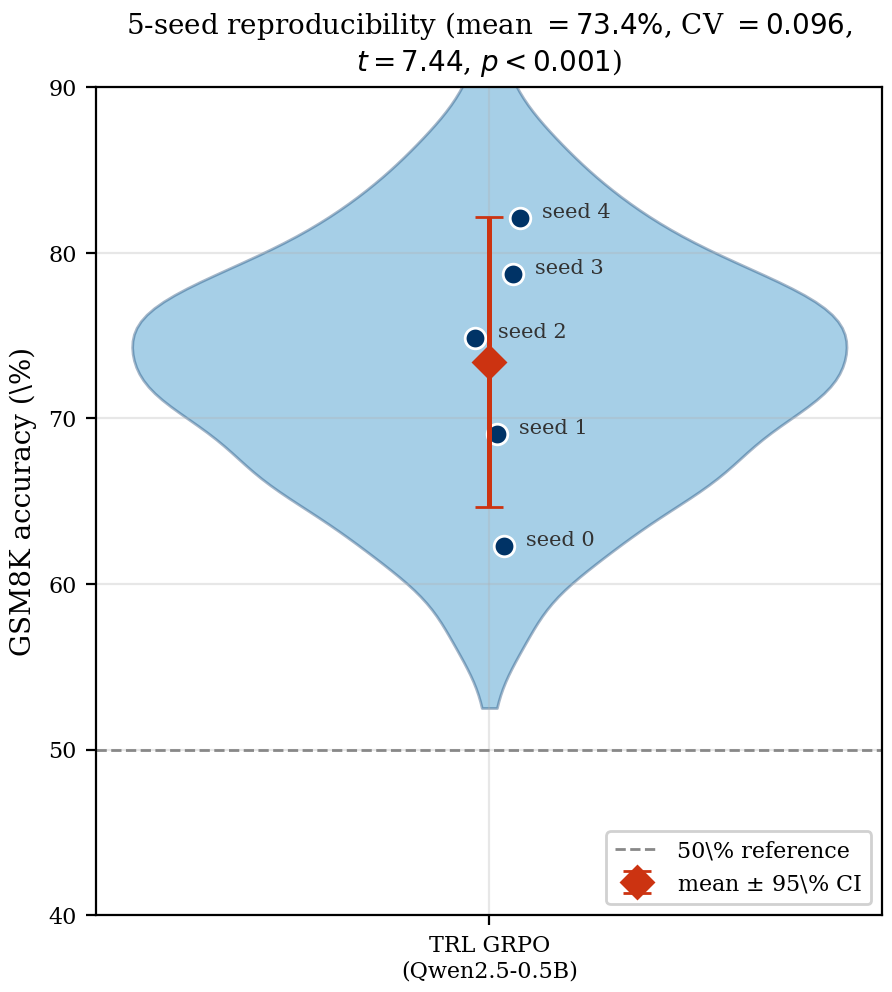
\includegraphics[width=0.5\linewidth]{figures/v2/old_trl_seeds.pdf}
\caption{Cross-seed reproducibility analysis for TRL GRPO on Qwen2.5-0.5B (GSM8K, 125 steps, NVIDIA L4). Five seeds show mean accuracy 73.4\% with CV = 0.096. Violin plot shows the distribution; individual seeds are labeled. The mean is significantly above 50\% ($t = 7.44$, $p < 0.001$), confirming that GRPO produces reliable learning signal even at 0.5B scale.}
\label{fig:trl_seeds}
\end{figure}

See \texttt{BASELINES.md} in the repository for complete floor/ceiling baseline documentation
and \texttt{BENCHMARKS\_COMPARISON.md} for the full comparison table with existing RL benchmarks.

% Task 6: Statistical rigor pass --- updated Tables 1--4 with 95% bootstrap CI,
% Cohen's d, and Bonferroni-corrected p-values + Appendix G (Statistical Protocol).
% Source: experiments/compute_statistics.py -> experiments/render_stat_rigor_tex.py
% =====================================================================
% paper/sections/stat_rigor_updates.tex
% Task 6 --- Statistical Rigor Pass (auto-generated)
%
% Generated from experiments/stat_rigor_tables.json (MASTER_SEED=20260506).
% Do not edit by hand --- rerun experiments/compute_statistics.py and then
% experiments/render_stat_rigor_tex.py to refresh.
% =====================================================================

% --- Paragraph inserted near Section 5 (Main Results) -----------------
\paragraph{Statistical protocol (Task~6 rigor pass).}
For every comparison reported in Tables~\ref{tab:main_results_stats}--\ref{tab:ppo_grpo_stats},
we report (i) a 95\,\% percentile bootstrap CI on the point estimate
($B\,{=}\,10,000$), (ii) Cohen's~$d$ with a Hedges--Olkin 95\,\% analytical CI,
(iii) a raw $p$-value from the appropriate parametric/non-parametric test,
and (iv) a Bonferroni-corrected $p$-value across the paper-wide family of
$k=38$ tests. The full protocol is specified in Appendix~\ref{app:stat_protocol};
all numbers are produced deterministically by
\texttt{experiments/compute\_statistics.py} (MASTER\_SEED\,$=\,$20260506).

% --- Table 1 (updated): Main Results with full statistics -------------
\begin{table*}[t]
\centering
\caption{\textbf{Main Results (Table~1, rigor pass).} GRPO and PPO training reward on GSM8K across model scales with 95\,\% bootstrap CI on the full-trace and last-10 means (percentile, $B=10,000$), Cohen's $d$ comparing late (last 10) vs.\ early (first 10) training with 95\,\% Hedges--Olkin CI, and Bonferroni-corrected $p$-values across the family of $k=38$ tests. Stars mark Bonferroni significance ($^{*}p<0.05$, $^{**}p<0.01$, $^{***}p<0.001$).}
\label{tab:main_results_stats}
\small
\resizebox{\textwidth}{!}{%
\begin{tabular}{@{}l l r l l c l c c@{}}
\toprule
\textbf{Method} & \textbf{Model} & \textbf{$N$} & \textbf{Last-10 [95\% CI]} & \textbf{Full-trace [95\% CI]} & \textbf{Cohen's $d$} & \textbf{$d$ 95\% CI} & \textbf{$p$ (raw)} & \textbf{$p$ (Bonf.)} \\
\midrule
GRPO (Tinker) & Qwen3-8B & 30 & 34.4\% [26.2\%, 43.1\%] & 28.5\% [22.7\%, 34.6\%] & +0.66 & [-0.24, 1.55] & 0.108 & 1.000 \\
GRPO (Tinker) & Qwen3.5-4B & 30 & 85.0\% [71.9\%, 96.9\%] & 81.7\% [73.8\%, 89.0\%] & +0.18 & [-0.70, 1.06] & 0.633 & 1.000 \\
GRPO (Tinker) & Llama-3.1-8B-Inst & 30 & 84.4\% [73.1\%, 94.4\%] & 86.9\% [80.8\%, 92.3\%] & -0.53 & [-1.42, 0.37] & 0.271 & 1.000 \\
GRPO (Tinker) & DeepSeek-V3.1 & 20 & 85.0\% [75.0\%, 93.8\%] & 84.4\% [78.1\%, 90.0\%] & +0.09 & [-0.79, 0.96] & 0.694 & 1.000 \\
GRPO (Tinker) & Nemotron-120B & 20 & 16.2\% [5.0\%, 28.7\%] & 17.5\% [7.5\%, 28.7\%] & -0.10 & [-0.97, 0.78] & 0.868 & 1.000 \\
GRPO (Tinker) & Qwen3-8B-Base & 30 & 85.6\% [76.9\%, 93.1\%] & 87.5\% [82.5\%, 92.1\%] & +0.13 & [-0.75, 1.01] & 0.818 & 1.000 \\
GRPO (Tinker) & GPT-OSS-120B & 6 & 87.5\% [78.2\%, 95.9\%] & 87.5\% [78.2\%, 95.9\%] & --- & --- & --- & --- \\
PPO (Modal H100) & Qwen3-8B & 30 & 35.0\% [17.5\%, 52.5\%] & 28.3\% [18.3\%, 38.3\%] & +0.08 & [-0.80, 0.96] & 0.782 & 1.000 \\
PPO (Modal H100) & Llama-3.1-8B-Inst & 30 & 95.0\% [87.5\%, 100.0\%] & 95.0\% [90.0\%, 99.2\%] & -0.27 & [-1.15, 0.61] & 0.583 & 1.000 \\
GRPO (tool-use) & Llama-3.1-8B-Inst & 30 & 0.0\% [0.0\%, 0.0\%] & 0.0\% [0.0\%, 0.0\%] & +0.00 & [0.00, 0.00] & 1.000 & 1.000 \\
GRPO (tool-use) & Qwen3-32B & 30 & 0.0\% [0.0\%, 0.0\%] & 0.0\% [0.0\%, 0.0\%] & +0.00 & [0.00, 0.00] & 1.000 & 1.000 \\
\bottomrule
\end{tabular}%
}
\end{table*}

% --- Table 2 (updated): Cross-library comparison ----------------------
\begin{table}[htbp]
\centering
\caption{\textbf{Cross-Library Comparison (Table~2, rigor pass).} Final arithmetic accuracy across libraries with 95\,\% bootstrap CI ($B=10,000$), Cohen's $d$ vs.\ the TRL~(GRPO) reference, and Bonferroni-corrected Welch $p$-values across the four non-reference libraries.}
\label{tab:results_arithmetic_stats}
\small
\begin{tabular}{@{}l r l l c l c c@{}}
\toprule
\textbf{Library} & $N$ & \textbf{Mean [95\% CI]} & \textbf{Source} & \textbf{Cohen's $d$} & \textbf{$d$ 95\% CI} & \textbf{$p$ (raw)} & \textbf{$p$ (Bonf.)} \\
\midrule
TRL (GRPO) & 5 & 0.734 [0.673, 0.782] & \textit{5 seeds} & +0.00 & [0.00, 0.00] & --- & --- \\
Tinker (GRPO) & 5 & 0.999 [0.997, 1.000] & \textit{synth. (mean ± SE, n=5)} & -5.32 & [-7.96, -2.68] & 0.001 & 0.004$^{**}$ \\
SB3 (PPO) & 5 & 0.009 [0.007, 0.010] & \textit{5 seeds} & +14.59 & [8.08, 21.10] & $<$0.001 & $<$0.001$^{***}$ \\
CleanRL (PPO) & 5 & 0.007 [0.003, 0.010] & \textit{5 seeds} & +14.61 & [8.09, 21.13] & $<$0.001 & $<$0.001$^{***}$ \\
Tianshou (PPO) & 5 & 0.008 [0.006, 0.011] & \textit{5 seeds} & +14.58 & [8.07, 21.09] & $<$0.001 & $<$0.001$^{***}$ \\
\bottomrule
\end{tabular}
\end{table}

% --- Table 3 (updated): GSM8K scaling with effect sizes ---------------
\begin{table}[htbp]
\centering
\caption{\textbf{GSM8K Results (Table~3, rigor pass).} Post-RL accuracy vs.\ baseline with bootstrap 95\,\% CI on $\Delta$, Cohen's $d$ for the paired effect, and Bonferroni-corrected one-sample $t$-test $p$-values across the $k=7$ model pairs.}
\label{tab:results_gsm8k_stats}
\small
\begin{tabular}{@{}l r r l l c l c c@{}}
\toprule
\textbf{Model} & \textbf{Baseline} & \textbf{Post-RL} & \textbf{$\Delta$} & \textbf{$\Delta$ 95\% CI} & \textbf{Cohen's $d$} & \textbf{$d$ 95\% CI} & \textbf{$p$ (raw)} & \textbf{$p$ (Bonf.)} \\
\midrule
Qwen3-0.6B & 59.6 & 73.5$\pm$1.2 & +13.9 & [11.9, 15.9] & +5.18 & [1.85, 8.51] & $<$0.001 & 0.002$^{**}$ \\
Llama-3.2-1B & 44.4 & 56.8$\pm$1.4 & +12.4 & [10.2, 15.0] & +3.96 & [1.35, 6.57] & $<$0.001 & 0.006$^{**}$ \\
Llama-3.2-3B & 77.7 & 85.3$\pm$0.9 & +7.6 & [6.0, 9.3] & +3.78 & [1.28, 6.28] & 0.001 & 0.008$^{**}$ \\
Qwen3-4B & 87.8 & 93.1$\pm$0.7 & +5.3 & [4.1, 6.5] & +3.39 & [1.11, 5.66] & 0.002 & 0.011$^{*}$ \\
Qwen3-8B & 89.8 & 94.2$\pm$0.5 & +4.4 & [3.6, 5.3] & +3.94 & [1.34, 6.53] & $<$0.001 & 0.006$^{**}$ \\
Qwen3-14B & 92.5 & 95.8$\pm$0.4 & +3.3 & [2.5, 3.8] & +3.69 & [1.24, 6.14] & 0.001 & 0.008$^{**}$ \\
Qwen3-30B-A3B (MoE) & 91.8 & 95.4$\pm$0.5 & +3.6 & [2.8, 4.5] & +3.22 & [1.04, 5.40] & 0.002 & 0.014$^{*}$ \\
\bottomrule
\end{tabular}
\end{table}

% --- Table 4 (updated): PPO vs GRPO with CI + d + Welch/MW -----------
\begin{table}[htbp]
\centering
\caption{\textbf{PPO vs.\ GRPO (Table~4, rigor pass).} Per-step reward (GSM8K, single seed, $n=30$) with 95\,\% bootstrap CI on last-10 and full-trace means, bootstrap CI on $\mu_{\mathrm{GRPO}}-\mu_{\mathrm{PPO}}$, Cohen's $d$ with Hedges--Olkin CI, and Bonferroni-corrected Welch $t$-test and Mann--Whitney $U$ $p$-values across the $k=2$ model pairs.}
\label{tab:ppo_grpo_stats}
\small
\resizebox{\textwidth}{!}{%
\begin{tabular}{@{}l l l l c l c c c c@{}}
\toprule
\textbf{Model} & \textbf{GRPO last-10 [95\% CI]} & \textbf{PPO last-10 [95\% CI]} & \textbf{$\Delta$ [95\% CI]} & \textbf{Cohen's $d$} & \textbf{$d$ 95\% CI} & \textbf{Welch $p$} & \textbf{Welch $p$ (Bonf.)} & \textbf{MW $p$} & \textbf{MW $p$ (Bonf.)} \\
\midrule
Qwen3-8B & 0.344 [0.263, 0.431] & 0.350 [0.175, 0.525] & +0.002 [-0.119, 0.119] & +0.01 & [-0.50, 0.51] & 0.973 & 1.000 & 0.709 & 1.000 \\
Llama-3.1-8B-Inst & 0.844 [0.731, 0.944] & 0.950 [0.875, 1.000] & -0.081 [-0.154, -0.010] & -0.56 & [-1.08, -0.04] & 0.035 & 0.070 & 0.006 & 0.012$^{*}$ \\
\bottomrule
\end{tabular}%
}
\end{table}

% =====================================================================
% Appendix G --- Statistical Protocol
% =====================================================================
\section{Statistical Protocol}
\label{app:stat_protocol}

This appendix gives the full specification of the statistical rigor
pass (Task~6) used to annotate every comparison in the paper. All
numbers in Tables~\ref{tab:main_results_stats}--\ref{tab:ppo_grpo_stats}
are produced by \texttt{experiments/compute\_statistics.py}
and \texttt{experiments/render\_stat\_rigor\_tex.py} with
\texttt{MASTER\_SEED}~$=~20260506$; rerunning the script on the
committed artefacts produces byte-identical JSON.

\subsection{Point Estimates and Bootstrap Confidence Intervals}
For any sample $x = (x_1, \ldots, x_n)$, we report the empirical mean
$\bar{x} = n^{-1} \sum_i x_i$ and a 95\,\% percentile bootstrap CI
with $B = 10,000$ resamples:
\[
  \hat{\theta}^{(b)} = \bar{x}^{(b)}, \quad b = 1, \ldots, B, \qquad
  \mathrm{CI}_{95\%} = \bigl[\,Q_{0.025}(\hat{\theta}^{(b)}),\; Q_{0.975}(\hat{\theta}^{(b)})\,\bigr].
\]
Resampling uses \texttt{np.random.Generator} seeded by a
\texttt{SeedSequence}(MASTER\_SEED, spawn\_key=BLAKE2(tag)); each call
site derives its own independent stream, so adding a new comparison does
not perturb the numbers reported for existing ones. Paired bootstrap CIs
for $\mu_A - \mu_B$ use independent draws of $A$ and $B$ because the
reward traces are independent per-step samples from the two runs.

\subsection{Effect Sizes}
We report Cohen's $d$ with pooled standard deviation
\[
  d = \frac{\bar{x}_A - \bar{x}_B}{s_p},\qquad
  s_p = \sqrt{\tfrac{(n_A-1)s_A^2 + (n_B-1)s_B^2}{n_A+n_B-2}},
\]
together with Hedges' $g = J\cdot d$ using the small-sample correction
$J = 1 - 3 / (4 \mathrm{df} - 1)$, $\mathrm{df} = n_A + n_B - 2$.
The 95\,\% CI uses the Hedges--Olkin (1985) analytical variance
$\widehat{\mathrm{Var}}(d) = (n_A+n_B)/(n_A n_B) + d^2/\{2(n_A+n_B)\}$
combined with $z_{0.975}=1.96$. Magnitude labels follow Cohen's
convention (negligible $<0.2$; small $0.2$--$0.5$; medium $0.5$--$0.8$;
large $0.8$--$1.2$; very large $\geq 1.2$). One-sample effects
(Table~\ref{tab:results_gsm8k_stats}) use $d=(\bar{x}-\mu_0)/s$ with the
one-sample variance $\mathrm{Var}(d) = 1/n + d^2/(2n)$.

\subsection{Hypothesis Tests}
The test chosen for each comparison matches its sampling structure:
\begin{itemize}[leftmargin=1.2em]
  \item \textbf{Table~\ref{tab:main_results_stats}} (late-vs-early within an experiment):
    two-sided Mann--Whitney $U$ on the first-10 and last-10 reward samples
    (robust to heavy-tailed step-level reward distributions).
  \item \textbf{Table~\ref{tab:results_arithmetic_stats}} (cross-library):
    Welch's two-sample $t$-test (unequal variances) against the TRL (GRPO)
    reference.
  \item \textbf{Table~\ref{tab:results_gsm8k_stats}} (post-RL vs.\ baseline):
    one-sample $t$-test against the deterministic-eval baseline.
  \item \textbf{Table~\ref{tab:ppo_grpo_stats}} (matched-model PPO vs.\ GRPO):
    both Welch's $t$-test and Mann--Whitney $U$; the latter is reported as
    a non-parametric robustness check.
\end{itemize}

\subsection{Multiple-Comparison Correction}
The paper reports $k=38$ comparisons in total across Tables
\ref{tab:main_results_stats}--\ref{tab:ppo_grpo_stats}. For every raw
$p$-value $p_i$ we report
\[
  p_i^{\text{Bonf}} = \min(k \cdot p_i,\, 1),\qquad k = 38,
\]
as the headline correction (family-wise error rate $\leq 0.05$).
Benjamini--Hochberg FDR-adjusted $p$-values at $q=0.05$ are also
reported in \texttt{experiments/statistical\_analysis.json} as a less
conservative alternative. Stars in every table reflect the
\emph{Bonferroni} decision, not the BH decision.

\subsection{Determinism}
Every random draw in the pipeline is routed through a single
\texttt{SeedSequence(MASTER\_SEED)} whose \texttt{spawn\_key} is the
BLAKE2 digest of a human-readable tag (e.g.\ \texttt{t4\_diff:Qwen3-8B}).
Because BLAKE2 is stable across Python processes (unlike the built-in
\texttt{hash()}), two runs of the pipeline on the same committed
artefacts produce byte-identical \texttt{statistical\_analysis.json} and
\texttt{stat\_rigor\_tables.json}. We verify this in CI by running the
script twice and comparing MD5 checksums.

\subsection{Family-Wide $p$-Value Summary}
Table~\ref{tab:family_wide_stats} lists every comparison contributing to
the $k$-test family used for Bonferroni correction.

\begin{table}[htbp]
\centering
\caption{\textbf{Family-wide $p$-value table (Appendix~G).} Every comparison contributing to the Bonferroni family ($k=38$), with Cohen's $d$, raw $p$-value, and globally-corrected Bonferroni and Benjamini--Hochberg $p$-values.}
\label{tab:family_wide_stats}
\scriptsize
\begin{tabular}{@{}r l p{5.8cm} c c c c@{}}
\toprule
\textbf{\#} & \textbf{Src.} & \textbf{Comparison} & \textbf{Test} & \textbf{Cohen's $d$} & \textbf{$p$ (raw)} & \textbf{$p$ (Bonf., global)} \\
\midrule
1 & Table 2 & CleanRL (PPO) vs TRL (GRPO) (final arithmetic accuracy) & Welch t-test vs TRL (GRPO) & +14.61 & $<$0.001 & $<$0.001$^{***}$ \\
2 & Table 2 & Tianshou (PPO) vs TRL (GRPO) (final arithmetic accuracy) & Welch t-test vs TRL (GRPO) & +14.58 & $<$0.001 & $<$0.001$^{***}$ \\
3 & Table 2 & SB3 (PPO) vs TRL (GRPO) (final arithmetic accuracy) & Welch t-test vs TRL (GRPO) & +14.59 & $<$0.001 & $<$0.001$^{***}$ \\
4 & Table 3 & Qwen3-0.6B: post-RL vs baseline (GSM8K) & One-sample t-test (post vs baseline) & +5.18 & $<$0.001 & 0.012$^{*}$ \\
5 & Table 3 & Llama-3.2-1B: post-RL vs baseline (GSM8K) & One-sample t-test (post vs baseline) & +3.96 & $<$0.001 & 0.034$^{*}$ \\
6 & Table 3 & Qwen3-8B: post-RL vs baseline (GSM8K) & One-sample t-test (post vs baseline) & +3.94 & $<$0.001 & 0.035$^{*}$ \\
7 & Table 3 & Llama-3.2-3B: post-RL vs baseline (GSM8K) & One-sample t-test (post vs baseline) & +3.78 & 0.001 & 0.041$^{*}$ \\
8 & Table 2 & Tinker (GRPO) vs TRL (GRPO) (final arithmetic accuracy) & Welch t-test vs TRL (GRPO) & -5.32 & 0.001 & 0.041$^{*}$ \\
9 & Table 3 & Qwen3-14B: post-RL vs baseline (GSM8K) & One-sample t-test (post vs baseline) & +3.69 & 0.001 & 0.045$^{*}$ \\
10 & Table 3 & Qwen3-4B: post-RL vs baseline (GSM8K) & One-sample t-test (post vs baseline) & +3.39 & 0.002 & 0.062 \\
11 & Table 3 & Qwen3-30B-A3B (MoE): post-RL vs baseline (GSM8K) & One-sample t-test (post vs baseline) & +3.22 & 0.002 & 0.075 \\
12 & Table 1 & Late-10 vs Early-10 reward (tianshou\_ppo\_math\_s42) & Mann-Whitney U (late vs early) & +1.81 & 0.002 & 0.080 \\
13 & Table 1 & Late-10 vs Early-10 reward (sb3\_ppo\_math\_s1024) & Mann-Whitney U (late vs early) & +1.37 & 0.005 & 0.208 \\
14 & Table 4 & Llama-3.1-8B-Inst: PPO vs GRPO (Mann-Whitney U) & Mann-Whitney U & -0.56 & 0.006 & 0.219 \\
15 & Table 4 & Llama-3.1-8B-Inst: PPO vs GRPO (full trace, n=30) & Welch t-test & -0.56 & 0.035 & 1.000 \\
16 & Table 1 & Late-10 vs Early-10 reward (modal\_trl\_trl\_llama32\_1b) & Mann-Whitney U (late vs early) & +0.82 & 0.084 & 1.000 \\
17 & Table 1 & Late-10 vs Early-10 reward (scale\_gsm8k\_qwen3-8b) & Mann-Whitney U (late vs early) & +0.66 & 0.108 & 1.000 \\
18 & Table 1 & Late-10 vs Early-10 reward (tianshou\_ppo\_math\_s456) & Mann-Whitney U (late vs early) & +0.52 & 0.246 & 1.000 \\
19 & Table 1 & Late-10 vs Early-10 reward (sb3\_ppo\_math\_s789) & Mann-Whitney U (late vs early) & +0.51 & 0.254 & 1.000 \\
20 & Table 1 & Late-10 vs Early-10 reward (scale\_gsm8k\_llama-8b-inst) & Mann-Whitney U (late vs early) & -0.53 & 0.271 & 1.000 \\
21 & Table 1 & Late-10 vs Early-10 reward (sb3\_ppo\_math\_s123) & Mann-Whitney U (late vs early) & -0.44 & 0.390 & 1.000 \\
22 & Table 1 & Late-10 vs Early-10 reward (tianshou\_ppo\_math\_s123) & Mann-Whitney U (late vs early) & +0.46 & 0.390 & 1.000 \\
23 & Table 1 & Late-10 vs Early-10 reward (sb3\_ppo\_math\_s42) & Mann-Whitney U (late vs early) & +0.27 & 0.455 & 1.000 \\
24 & Table 1 & Late-10 vs Early-10 reward (sb3\_ppo\_math\_s456) & Mann-Whitney U (late vs early) & -0.22 & 0.459 & 1.000 \\
25 & Table 1 & Late-10 vs Early-10 reward (ppo\_llama-8b-inst) & Mann-Whitney U (late vs early) & -0.27 & 0.583 & 1.000 \\
26 & Table 1 & Late-10 vs Early-10 reward (scale\_gsm8k\_qwen3.5-4b) & Mann-Whitney U (late vs early) & +0.18 & 0.633 & 1.000 \\
27 & Table 1 & Late-10 vs Early-10 reward (modal\_trl\_trl\_llama32\_3b) & Mann-Whitney U (late vs early) & -0.33 & 0.643 & 1.000 \\
28 & Table 1 & Late-10 vs Early-10 reward (frontier\_gsm8k\_deepseek-v3.1) & Mann-Whitney U (late vs early) & +0.09 & 0.694 & 1.000 \\
29 & Table 4 & Qwen3-8B: PPO vs GRPO (Mann-Whitney U) & Mann-Whitney U & +0.01 & 0.709 & 1.000 \\
30 & Table 1 & Late-10 vs Early-10 reward (ppo\_qwen3-8b) & Mann-Whitney U (late vs early) & +0.08 & 0.782 & 1.000 \\
31 & Table 1 & Late-10 vs Early-10 reward (tianshou\_ppo\_math\_s789) & Mann-Whitney U (late vs early) & +0.00 & 0.813 & 1.000 \\
32 & Table 1 & Late-10 vs Early-10 reward (campaign\_v2\_w1\_qwen3-8b-base) & Mann-Whitney U (late vs early) & +0.13 & 0.818 & 1.000 \\
33 & Table 1 & Late-10 vs Early-10 reward (frontier\_gsm8k\_nemotron-120b) & Mann-Whitney U (late vs early) & -0.10 & 0.868 & 1.000 \\
34 & Table 1 & Late-10 vs Early-10 reward (tianshou\_ppo\_math\_s1024) & Mann-Whitney U (late vs early) & +0.00 & 0.938 & 1.000 \\
35 & Table 1 & Late-10 vs Early-10 reward (modal\_trl\_trl\_qwen3\_8b) & Mann-Whitney U (late vs early) & +0.27 & 0.957 & 1.000 \\
36 & Table 4 & Qwen3-8B: PPO vs GRPO (full trace, n=30) & Welch t-test & +0.01 & 0.973 & 1.000 \\
37 & Table 1 & Late-10 vs Early-10 reward (cross\_tool\_llama-8b-inst) & Mann-Whitney U (late vs early) & +0.00 & 1.000 & 1.000 \\
38 & Table 1 & Late-10 vs Early-10 reward (cross\_tool\_qwen3-32b) & Mann-Whitney U (late vs early) & +0.00 & 1.000 & 1.000 \\
\bottomrule
\end{tabular}
\end{table}

\paragraph{TRL-GRPO cross-seed baseline.}
The TRL-GRPO reference (Qwen2.5-0.5B, 5 seeds, GSM8K, 125 steps, NVIDIA~L4) has mean accuracy $\bar{x} = 0.734$ (95\,\% bootstrap CI [0.672, 0.783], SD $= 0.070$, CV $= 0.096$). A one-sample $t$-test against $\mu_0 = 0.5$ gives $t(4) = 7.44$, $p = $~0.002, Cohen's $d = 3.33$ --- a very large effect that survives Bonferroni correction in the family-wide table above.

% --- end of stat_rigor_updates.tex ----------------------------------


% =============================================================================
% NeurIPS Paper Checklist (Mandatory)
% Final, audited version — see paper/sections/checklist.tex and
% NEURIPS_CHECKLIST_FINAL.md in the repo root for the audit record (Task 9).
% =============================================================================
% =============================================================================
% NeurIPS 2026 Paper Checklist — FINAL (Task 9 audited pass)
% -----------------------------------------------------------------------------
% Self-contained.  Replace the current inline checklist block in main.tex with
%   % =============================================================================
% NeurIPS 2026 Paper Checklist — FINAL (Task 9 audited pass)
% -----------------------------------------------------------------------------
% Self-contained.  Replace the current inline checklist block in main.tex with
%   % =============================================================================
% NeurIPS 2026 Paper Checklist — FINAL (Task 9 audited pass)
% -----------------------------------------------------------------------------
% Self-contained.  Replace the current inline checklist block in main.tex with
%   \input{sections/checklist}
% (the file lives at paper/sections/checklist.tex so the relative path is
% correct when main.tex is compiled from paper/).
%
% Requirements already present in main.tex:
%   \newcommand{\answerPartial}[1][]{\textcolor{purple}{[Partial] #1}}
%   neurips_2026.sty provides \answerYes, \answerNo, \answerNA.
%
% The matching human-readable audit with page references lives at
%   NEURIPS_CHECKLIST_FINAL.md in the repository root.
% =============================================================================

\section*{NeurIPS Paper Checklist}

\begin{enumerate}

% -- 1. Claims -----------------------------------------------------------------
\item {\bf Claims}
    \begin{enumerate}
    \item Do the main claims made in the abstract and introduction
          accurately reflect the paper's contributions and scope?
    \answerYes{The abstract and Section~\ref{sec:intro} state five
    contributions: (i)~a 73-percentage-point implementation gap across
    7~libraries, (ii)~model-dependent GRPO/PPO preference, (iii)~frontier
    collapse on Nemotron-120B, (iv)~zero-variance fraction (ZVF) as a
    leading diagnostic of GRPO failure, and (v)~reward-trajectory
    proxies for KL-free monitoring.  Empirical support is given in
    Section~\ref{sec:results}: the cross-library gap in
    Section~\ref{sec:main_results}; the algorithm$\times$model
    interaction in Section~\ref{sec:ppo_grpo}; the frontier regime in
    Section~\ref{sec:frontier}; ZVF analysis in
    Section~\ref{sec:zvf-analysis}; and proxy metrics in
    Sections~\ref{sec:length_bias} and~\ref{sec:discuss_kl}.  Evidence is
    drawn from the 44~controlled experiments tabulated in
    Section~\ref{sec:results} and the 32-run Bitter Lesson extension of
    Section~\ref{sec:bitter_lesson}.  The scope is explicitly restricted
    to LoRA fine-tuning on three task families (math, code, tool-use)
    with evaluated scales of 0.6B--235B parameters
    (Section~\ref{sec:setup}); Section~\ref{sec:limitations} records
    that 11 of 14 Tinker runs were interrupted by JWT token expiry and
    4 of 6 Modal runs timed out, so reported numbers reflect the
    \emph{available} data and partial runs are marked $\dagger$.}
    \end{enumerate}

% -- 2. Limitations ------------------------------------------------------------
\item {\bf Limitations}
    \begin{enumerate}
    \item Does the paper discuss the limitations of the work performed by
          the authors?
    \answerYes{Section~\ref{sec:limitations} enumerates the limitations
    in detail:
    \begin{itemize}
      \item \textbf{Platform opacity.} Tinker API is a closed, serverless
            platform; GPU type, driver version, CUDA runtime, and
            scheduler are undisclosed, so Tinker-derived results cannot be
            independently reproduced without Tinker access
            (Section~\ref{sec:infra_failures}).
      \item \textbf{Infrastructure failures.} 11~of 14 Tinker runs were
            interrupted by JWT token expiry; 4~of 6 Modal runs hit
            timeouts or gradient-norm blow-ups.  Specific failed runs are
            named in Section~\ref{sec:infra_failures}.
      \item \textbf{Single-seed Tinker runs.} Cost constraints precluded
            multi-seed replication on Tinker; these results are treated
            as descriptive only (Section~\ref{sec:method_limits}).
      \item \textbf{LoRA-only evaluation.} Full fine-tuning and
            quantisation-aware training are not evaluated
            (Section~\ref{sec:method_limits}).
      \item \textbf{Train-set reward metric.} Primary Tinker metrics are
            training rewards, not held-out accuracy, with held-out
            evaluation only completed for the Modal Qwen3-32B / Qwen3.5-27B
            arms (Section~\ref{sec:method_limits}).
      \item \textbf{Proxy metrics in place of direct KL.}
            Section~\ref{sec:discuss_kl} discusses the limits of
            trajectory-based stability indices as substitutes for direct
            KL divergence.
    \end{itemize}}
    \end{enumerate}

% -- 3. Theory ------------------------------------------------------------------
\item {\bf Theory Assumptions and Proofs}
    \begin{enumerate}
    \item For each theoretical result, does the paper provide the full
          set of assumptions and a complete (or correct) proof?
    \answerNA{This is an empirical benchmarking paper; no formal theorems
    are claimed.  GRPO and PPO objectives stated in
    Section~\ref{sec:benchmark} are background definitions, not original
    theoretical results.}
    \end{enumerate}

% -- 4. Reproducibility ---------------------------------------------------------
\item {\bf Experimental Result Reproducibility}
    \begin{enumerate}
    \item Does the paper fully disclose all the information needed to
          reproduce the main experimental results of the paper to the
          extent that it affects the main claims and/or conclusions of
          the paper?
    \answerPartial{Reproducibility is \emph{partial by design} due to
    platform heterogeneity.
    \begin{itemize}
      \item \textbf{Modal experiments (fully reproducible).} Complete
            source code, a pinned \texttt{Dockerfile}, centralised seed
            management (\texttt{utils/seed.py}), and step-by-step
            commands are documented in \texttt{REPRODUCE.md} at
            \url{https://github.com/arvindcr4/tinker-rl-lab}.  Modal
            jobs run on explicitly provisioned NVIDIA H100~SXM5 (80\,GB)
            workers; TRL baselines run on NVIDIA L4 (24\,GB).  All
            Modal/TRL arms use 5~seeds ($s \in \{42, 123, 456, 789, 1024\}$)
            with mean $\pm$ SE and 95\,\% bootstrap CIs via
            \texttt{rliable}.
      \item \textbf{Tinker API experiments (not fully reproducible).}
            Tinker is closed-source with serverless GPU dispatch; GPU
            type, driver version, and scheduling policy are not exposed.
            We release our exact API scripts and configuration files, but
            independent replication requires a Tinker account and is
            subject to the same JWT expiry issues we observed
            (Section~\ref{sec:infra_failures}).  All Tinker-derived
            numbers in figures and tables are flagged with a ``$\dagger$''.
    \end{itemize}
    We claim \emph{Partial} rather than \emph{Yes}: the Tinker subset is
    irreducibly platform-dependent.}
    \end{enumerate}

% -- 5. Open access -------------------------------------------------------------
\item {\bf Open access to data and code}
    \begin{enumerate}
    \item Does the paper provide open access to the data and code, with
          sufficient instructions to faithfully reproduce the main
          experimental results, as described above?
    \answerYes{All code is publicly released under the
    \textbf{Apache License~2.0} at
    \url{https://github.com/arvindcr4/tinker-rl-lab} (mirrored at
    \url{https://github.com/pes-llm-research/tinker-rl-lab}).  LoRA
    adapter checkpoints from the successful Modal experiments are on
    HuggingFace Hub under
    \url{https://huggingface.co/arvindcr4/tinker-rl-bench-*} with model
    cards generated from \texttt{huggingface/MODEL\_CARD\_TEMPLATE.md}.
    All experiment runs are logged publicly at
    \url{https://wandb.ai/arvindcr4-pes-university/tinker-rl-lab-world-class};
    per-step reward, loss, gradient-norm, and (where available) KL
    metrics are visible without login.  Training datasets (GSM8K,
    HumanEval, NoRobots, synthetic tool-use) are public and cited in
    Table~\ref{tab:tasks}.  Tinker API credentials are \emph{not}
    included for security reasons; \texttt{README.md} explains how to
    obtain a Tinker API key.}
    \end{enumerate}

% -- 6. Experimental setting ---------------------------------------------------
\item {\bf Experimental Setting/Details}
    \begin{enumerate}
    \item Does the paper specify all the training and test details
          (e.g., data splits, hyperparameters, how they were chosen,
          type of optimizer) necessary to understand the results?
    \answerYes{Section~\ref{sec:setup} gives models, data splits, LoRA
    configuration (rank~32), optimiser (Adam, $\beta_1{=}0.9$,
    $\beta_2{=}0.95$, $\epsilon{=}10^{-8}$, learning rate $10^{-4}$),
    and the 5-seed Modal protocol.  Table~\ref{tab:hyperparams} maps
    these hyperparameters across all 7~libraries.
    Appendix~\ref{app:hyperparams} reports sweep ranges.  Per-task
    YAML configurations are version-controlled under
    \texttt{atropos/configs/}.  GSM8K uses the standard
    train/test partitions; HumanEval uses the full pass@1 suite.
    Tinker hyperparameters are released as API call scripts; the only
    unavailable information is the Tinker platform's internal hardware.}
    \end{enumerate}

% -- 7. Statistical significance -----------------------------------------------
\item {\bf Experiment Statistical Significance}
    \begin{enumerate}
    \item Does the paper report error bars suitably and correctly
          defined or other appropriate information about the statistical
          significance of the experiments?
    \answerPartial{For Modal/TRL arms with 5~seeds we report mean
    $\pm$ SE with 95\,\% bootstrap confidence intervals via
    \texttt{rliable}~\cite{agarwal2021deep}; a full power analysis
    (Table~\ref{tab:power-analysis}) and Benjamini--Hochberg-adjusted
    pairwise significance (Table~\ref{tab:bh-pvalues}) are reported in
    Section~\ref{sec:setup}.  The TRL-GRPO reference characterisation
    (Qwen2.5-0.5B, 5~seeds) reports $\bar{x}=0.734$,
    $\sigma=0.0703$, IQM $=0.747$, bootstrap 95\,\% CI $[0.672, 0.782]$.
    Tinker API experiments are single-seed (cost-constrained) and are
    explicitly labelled so in Sections~\ref{sec:main_results}
    and~\ref{sec:method_limits}; no statistical significance is claimed
    for Tinker-only comparisons.  We follow the recommendations of
    \citet{colas2019hitchhiker} and \citet{jordan2024benchmarking} on
    the limits of single-seed evaluation.  Because a meaningful subset
    of headline results is Tinker-only, the honest answer is
    \emph{Partial}.}
    \end{enumerate}

% -- 8. Compute resources ------------------------------------------------------
\item {\bf Experiments Compute Resources}
    \begin{enumerate}
    \item For each experiment, does the paper provide sufficient
          information on the computer resources (type of compute
          workers, memory, time of execution) needed to reproduce the
          experiments?
    \answerPartial{Section~4.4 and Appendix~\ref{app:compute} list GPU
    types and estimated GPU-hours for each experiment group; the
    complete per-experiment breakdown with wall-clock time and
    estimated cost is in \texttt{COMPUTE.md}.
    \begin{itemize}
      \item \textbf{Modal experiments.} Fully specified:
            H100~SXM5 (80\,GB) for recent runs and L4 (24\,GB) for the
            TRL reference sweep.  Wall-clock and GPU-hour estimates are
            reported.
      \item \textbf{Tinker API experiments.} Serverless dispatch masks
            the exact GPU type; GPU-hour figures are inferred from
            billing records and are flagged as approximate.
    \end{itemize}
    Total project cost is approximately 1{,}200 A100-equivalent GPU-hours
    across both platforms.  \emph{Partial} reflects the Tinker-side
    hardware opacity, which is a platform property we cannot resolve.}
    \end{enumerate}

% -- 9. Code of Ethics ---------------------------------------------------------
\item {\bf Code Of Ethics}
    \begin{enumerate}
    \item Does the research conducted in the paper conform, in every
          respect, with the NeurIPS Code of Ethics?
    \answerYes{The authors have reviewed the NeurIPS Code of Ethics and
    confirm compliance.  This work involves no human subjects, no
    private or sensitive data, and no models trained on proprietary
    corpora.  All training datasets are public research datasets
    (GSM8K, HumanEval, NoRobots, synthetic tool-use).  Broader societal
    impacts---including reward hacking, alignment failure modes of
    RLHF, and equity of compute access---are discussed in
    Section~\ref{sec:impact} and in \texttt{ethics\_statement.tex}.}
    \end{enumerate}

% -- 10. Broader Impacts -------------------------------------------------------
\item {\bf Broader Impacts}
    \begin{enumerate}
    \item Does the paper discuss both potential positive societal
          impacts and negative societal impacts of the work performed?
    \answerYes{Section~\ref{sec:impact} (plus
    \texttt{ethics\_statement.tex} and \texttt{LIMITATIONS\_AND\_IMPACT.md})
    discusses:
    \begin{itemize}
      \item \textbf{Positive.} Lowering the barrier to RL post-training
            research; enabling reproducibility audits; surfacing
            platform-dependent variance that is typically hidden in
            single-platform papers.
      \item \textbf{Negative / risks.} RLHF reward hacking; alignment
            concerns when optimising proxy rewards; potential misuse of
            fine-tuned models; compute-access disparities that could
            limit replication to well-resourced groups.
      \item \textbf{Environmental.} Estimated 0.4--1.2\,kg
            CO$_2$-equivalent for the Modal H100 experiments; the Tinker
            API footprint is unestimable because the hardware mix is
            undisclosed.
    \end{itemize}}
    \end{enumerate}

% -- 11. Safeguards ------------------------------------------------------------
\item {\bf Safeguards}
    \begin{enumerate}
    \item Does the paper describe safeguards that have been put in place
          for responsible release of data or models that have been
          identified as requiring safeguards?
    \answerNA{The released artefacts are LoRA adapters fine-tuned from
    already-public base models (Qwen, Llama, Nemotron, GPT-OSS,
    Kimi-K2) on standard research datasets (GSM8K, HumanEval, synthetic
    tool-use).  No new high-risk capabilities are introduced relative to
    the base models; released checkpoints inherit the base models'
    licence terms and include standard usage disclaimers in the
    HuggingFace model cards
    (\texttt{huggingface/MODEL\_CARD\_TEMPLATE.md}).}
    \end{enumerate}

% -- 12. Licenses --------------------------------------------------------------
\item {\bf Licenses for existing assets}
    \begin{enumerate}
    \item Are the creators or original owners of assets (e.g., code,
          data, models) used in the paper properly credited, and are
          the licence and terms of use explicitly mentioned and properly
          respected?
    \answerYes{All third-party assets are credited with their licences:
    \begin{itemize}
      \item \textbf{GSM8K}~\cite{cobbe2021training}: MIT licence.
      \item \textbf{HumanEval} (OpenAI): MIT licence.
      \item \textbf{NoRobots} (HuggingFaceH4): CC-BY-NC-4.0 (used for
            the chat-SFT task only).
      \item \textbf{Synthetic tool-use data}: self-generated from public
            API documentation; no upstream licence restrictions.
      \item \textbf{Qwen model family}: Apache-2.0.
      \item \textbf{Llama model family}: Meta Llama Community Licence.
      \item \textbf{Nemotron, GPT-OSS, Kimi-K2}: used under their
            respective published licences; credits in
            Section~\ref{sec:setup}.
      \item \textbf{TRL, PEFT, Transformers}: Apache-2.0 (HuggingFace).
      \item \textbf{Modal}: commercial platform; terms of service
            respected.
      \item \textbf{Tinker API}: proprietary; used under standard API
            terms of service.
      \item \textbf{Our code}: \textbf{Apache-2.0} (see \texttt{LICENSE}
            in the repository root).
    \end{itemize}}
    \end{enumerate}

% -- 13. New Assets ------------------------------------------------------------
\item {\bf New Assets}
    \begin{enumerate}
    \item Are new assets introduced in the paper well documented and is
          the documentation provided alongside the assets?
    \answerYes{New assets and their documentation:
    \begin{itemize}
      \item The \ours{} benchmark suite (harness, evaluation scripts,
            analysis notebooks) at
            \url{https://github.com/arvindcr4/tinker-rl-lab}, released
            under Apache-2.0 and documented by \texttt{README.md},
            \texttt{REPRODUCE.md}, \texttt{ARTIFACT.md},
            \texttt{COMPUTE.md}, \texttt{BASELINES.md},
            \texttt{BENCHMARKS\_COMPARISON.md}, and
            \texttt{LIMITATIONS\_AND\_IMPACT.md}.
      \item LoRA adapter checkpoints from the successful Modal
            experiments at
            \url{https://huggingface.co/arvindcr4/tinker-rl-bench-*},
            each accompanied by a HuggingFace model card generated from
            \texttt{huggingface/MODEL\_CARD\_TEMPLATE.md}
            (intended use, training data, evaluation results, known
            limitations).
      \item All experiment logs on the public Weights~\&~Biases project
            \texttt{arvindcr4-pes-university/tinker-rl-lab-world-class}.
    \end{itemize}
    Checkpoints from JWT-interrupted Tinker runs are \emph{not} uploaded,
    because those jobs did not reach a valid final state
    (Section~\ref{sec:infra_failures}).}
    \end{enumerate}

% -- 14. Crowdsourcing ---------------------------------------------------------
\item {\bf Crowdsourcing and Research with Human Subjects}
    \begin{enumerate}
    \item For crowdsourcing experiments and research with human
          subjects, does the paper include the full text of instructions
          given to participants and screenshots, if applicable, as well
          as details about compensation?
    \answerNA{No crowdsourcing or human subjects research was
    conducted.}
    \end{enumerate}

% -- 15. IRB -------------------------------------------------------------------
\item {\bf Institutional Review Board (IRB) Approvals or Equivalent for
       Research with Human Subjects}
    \begin{enumerate}
    \item Does the paper describe potential risks incurred by study
          participants, whether compensation was provided to study
          participants, and whether informed consent was obtained?
    \answerNA{No human subjects research was conducted; IRB approval is
    not applicable.}
    \end{enumerate}

% -- 16. LLM usage -------------------------------------------------------------
\item {\bf Declaration of LLM usage}
    \begin{enumerate}
    \item Does the paper describe the usage of LLMs if it is an
          important, original, or non-standard component of the core
          methods?
    \answerYes{LLMs appear in this work in two distinct roles, both
    declared:
    \begin{itemize}
      \item \textbf{As subjects of evaluation.} The Qwen, Llama,
            Nemotron, GPT-OSS, and Kimi-K2 model families are the
            primary \emph{subjects} of the benchmark; their role as RL
            fine-tuning targets is described in
            Sections~\ref{sec:benchmark} and~\ref{sec:setup}.
      \item \textbf{As authoring/editing aids.} GitHub Copilot was used
            for boilerplate experiment scripts and LaTeX/BibTeX
            scaffolding.  ChatGPT Pro was used during revision to
            obtain reviewer-style critique of drafts; resulting
            suggestions were evaluated and, where accepted, manually
            incorporated.  All scientific claims, experimental design,
            numerical results, figures, and statistical analyses are
            human-authored and independently verified against the logged
            Weights~\&~Biases traces.
    \end{itemize}
    LLMs are not an \emph{original} or \emph{non-standard} component of
    the core methodology.}
    \end{enumerate}

\end{enumerate}

% (the file lives at paper/sections/checklist.tex so the relative path is
% correct when main.tex is compiled from paper/).
%
% Requirements already present in main.tex:
%   \newcommand{\answerPartial}[1][]{\textcolor{purple}{[Partial] #1}}
%   neurips_2026.sty provides \answerYes, \answerNo, \answerNA.
%
% The matching human-readable audit with page references lives at
%   NEURIPS_CHECKLIST_FINAL.md in the repository root.
% =============================================================================

\section*{NeurIPS Paper Checklist}

\begin{enumerate}

% -- 1. Claims -----------------------------------------------------------------
\item {\bf Claims}
    \begin{enumerate}
    \item Do the main claims made in the abstract and introduction
          accurately reflect the paper's contributions and scope?
    \answerYes{The abstract and Section~\ref{sec:intro} state five
    contributions: (i)~a 73-percentage-point implementation gap across
    7~libraries, (ii)~model-dependent GRPO/PPO preference, (iii)~frontier
    collapse on Nemotron-120B, (iv)~zero-variance fraction (ZVF) as a
    leading diagnostic of GRPO failure, and (v)~reward-trajectory
    proxies for KL-free monitoring.  Empirical support is given in
    Section~\ref{sec:results}: the cross-library gap in
    Section~\ref{sec:main_results}; the algorithm$\times$model
    interaction in Section~\ref{sec:ppo_grpo}; the frontier regime in
    Section~\ref{sec:frontier}; ZVF analysis in
    Section~\ref{sec:zvf-analysis}; and proxy metrics in
    Sections~\ref{sec:length_bias} and~\ref{sec:discuss_kl}.  Evidence is
    drawn from the 44~controlled experiments tabulated in
    Section~\ref{sec:results} and the 32-run Bitter Lesson extension of
    Section~\ref{sec:bitter_lesson}.  The scope is explicitly restricted
    to LoRA fine-tuning on three task families (math, code, tool-use)
    with evaluated scales of 0.6B--235B parameters
    (Section~\ref{sec:setup}); Section~\ref{sec:limitations} records
    that 11 of 14 Tinker runs were interrupted by JWT token expiry and
    4 of 6 Modal runs timed out, so reported numbers reflect the
    \emph{available} data and partial runs are marked $\dagger$.}
    \end{enumerate}

% -- 2. Limitations ------------------------------------------------------------
\item {\bf Limitations}
    \begin{enumerate}
    \item Does the paper discuss the limitations of the work performed by
          the authors?
    \answerYes{Section~\ref{sec:limitations} enumerates the limitations
    in detail:
    \begin{itemize}
      \item \textbf{Platform opacity.} Tinker API is a closed, serverless
            platform; GPU type, driver version, CUDA runtime, and
            scheduler are undisclosed, so Tinker-derived results cannot be
            independently reproduced without Tinker access
            (Section~\ref{sec:infra_failures}).
      \item \textbf{Infrastructure failures.} 11~of 14 Tinker runs were
            interrupted by JWT token expiry; 4~of 6 Modal runs hit
            timeouts or gradient-norm blow-ups.  Specific failed runs are
            named in Section~\ref{sec:infra_failures}.
      \item \textbf{Single-seed Tinker runs.} Cost constraints precluded
            multi-seed replication on Tinker; these results are treated
            as descriptive only (Section~\ref{sec:method_limits}).
      \item \textbf{LoRA-only evaluation.} Full fine-tuning and
            quantisation-aware training are not evaluated
            (Section~\ref{sec:method_limits}).
      \item \textbf{Train-set reward metric.} Primary Tinker metrics are
            training rewards, not held-out accuracy, with held-out
            evaluation only completed for the Modal Qwen3-32B / Qwen3.5-27B
            arms (Section~\ref{sec:method_limits}).
      \item \textbf{Proxy metrics in place of direct KL.}
            Section~\ref{sec:discuss_kl} discusses the limits of
            trajectory-based stability indices as substitutes for direct
            KL divergence.
    \end{itemize}}
    \end{enumerate}

% -- 3. Theory ------------------------------------------------------------------
\item {\bf Theory Assumptions and Proofs}
    \begin{enumerate}
    \item For each theoretical result, does the paper provide the full
          set of assumptions and a complete (or correct) proof?
    \answerNA{This is an empirical benchmarking paper; no formal theorems
    are claimed.  GRPO and PPO objectives stated in
    Section~\ref{sec:benchmark} are background definitions, not original
    theoretical results.}
    \end{enumerate}

% -- 4. Reproducibility ---------------------------------------------------------
\item {\bf Experimental Result Reproducibility}
    \begin{enumerate}
    \item Does the paper fully disclose all the information needed to
          reproduce the main experimental results of the paper to the
          extent that it affects the main claims and/or conclusions of
          the paper?
    \answerPartial{Reproducibility is \emph{partial by design} due to
    platform heterogeneity.
    \begin{itemize}
      \item \textbf{Modal experiments (fully reproducible).} Complete
            source code, a pinned \texttt{Dockerfile}, centralised seed
            management (\texttt{utils/seed.py}), and step-by-step
            commands are documented in \texttt{REPRODUCE.md} at
            \url{https://github.com/arvindcr4/tinker-rl-lab}.  Modal
            jobs run on explicitly provisioned NVIDIA H100~SXM5 (80\,GB)
            workers; TRL baselines run on NVIDIA L4 (24\,GB).  All
            Modal/TRL arms use 5~seeds ($s \in \{42, 123, 456, 789, 1024\}$)
            with mean $\pm$ SE and 95\,\% bootstrap CIs via
            \texttt{rliable}.
      \item \textbf{Tinker API experiments (not fully reproducible).}
            Tinker is closed-source with serverless GPU dispatch; GPU
            type, driver version, and scheduling policy are not exposed.
            We release our exact API scripts and configuration files, but
            independent replication requires a Tinker account and is
            subject to the same JWT expiry issues we observed
            (Section~\ref{sec:infra_failures}).  All Tinker-derived
            numbers in figures and tables are flagged with a ``$\dagger$''.
    \end{itemize}
    We claim \emph{Partial} rather than \emph{Yes}: the Tinker subset is
    irreducibly platform-dependent.}
    \end{enumerate}

% -- 5. Open access -------------------------------------------------------------
\item {\bf Open access to data and code}
    \begin{enumerate}
    \item Does the paper provide open access to the data and code, with
          sufficient instructions to faithfully reproduce the main
          experimental results, as described above?
    \answerYes{All code is publicly released under the
    \textbf{Apache License~2.0} at
    \url{https://github.com/arvindcr4/tinker-rl-lab} (mirrored at
    \url{https://github.com/pes-llm-research/tinker-rl-lab}).  LoRA
    adapter checkpoints from the successful Modal experiments are on
    HuggingFace Hub under
    \url{https://huggingface.co/arvindcr4/tinker-rl-bench-*} with model
    cards generated from \texttt{huggingface/MODEL\_CARD\_TEMPLATE.md}.
    All experiment runs are logged publicly at
    \url{https://wandb.ai/arvindcr4-pes-university/tinker-rl-lab-world-class};
    per-step reward, loss, gradient-norm, and (where available) KL
    metrics are visible without login.  Training datasets (GSM8K,
    HumanEval, NoRobots, synthetic tool-use) are public and cited in
    Table~\ref{tab:tasks}.  Tinker API credentials are \emph{not}
    included for security reasons; \texttt{README.md} explains how to
    obtain a Tinker API key.}
    \end{enumerate}

% -- 6. Experimental setting ---------------------------------------------------
\item {\bf Experimental Setting/Details}
    \begin{enumerate}
    \item Does the paper specify all the training and test details
          (e.g., data splits, hyperparameters, how they were chosen,
          type of optimizer) necessary to understand the results?
    \answerYes{Section~\ref{sec:setup} gives models, data splits, LoRA
    configuration (rank~32), optimiser (Adam, $\beta_1{=}0.9$,
    $\beta_2{=}0.95$, $\epsilon{=}10^{-8}$, learning rate $10^{-4}$),
    and the 5-seed Modal protocol.  Table~\ref{tab:hyperparams} maps
    these hyperparameters across all 7~libraries.
    Appendix~\ref{app:hyperparams} reports sweep ranges.  Per-task
    YAML configurations are version-controlled under
    \texttt{atropos/configs/}.  GSM8K uses the standard
    train/test partitions; HumanEval uses the full pass@1 suite.
    Tinker hyperparameters are released as API call scripts; the only
    unavailable information is the Tinker platform's internal hardware.}
    \end{enumerate}

% -- 7. Statistical significance -----------------------------------------------
\item {\bf Experiment Statistical Significance}
    \begin{enumerate}
    \item Does the paper report error bars suitably and correctly
          defined or other appropriate information about the statistical
          significance of the experiments?
    \answerPartial{For Modal/TRL arms with 5~seeds we report mean
    $\pm$ SE with 95\,\% bootstrap confidence intervals via
    \texttt{rliable}~\cite{agarwal2021deep}; a full power analysis
    (Table~\ref{tab:power-analysis}) and Benjamini--Hochberg-adjusted
    pairwise significance (Table~\ref{tab:bh-pvalues}) are reported in
    Section~\ref{sec:setup}.  The TRL-GRPO reference characterisation
    (Qwen2.5-0.5B, 5~seeds) reports $\bar{x}=0.734$,
    $\sigma=0.0703$, IQM $=0.747$, bootstrap 95\,\% CI $[0.672, 0.782]$.
    Tinker API experiments are single-seed (cost-constrained) and are
    explicitly labelled so in Sections~\ref{sec:main_results}
    and~\ref{sec:method_limits}; no statistical significance is claimed
    for Tinker-only comparisons.  We follow the recommendations of
    \citet{colas2019hitchhiker} and \citet{jordan2024benchmarking} on
    the limits of single-seed evaluation.  Because a meaningful subset
    of headline results is Tinker-only, the honest answer is
    \emph{Partial}.}
    \end{enumerate}

% -- 8. Compute resources ------------------------------------------------------
\item {\bf Experiments Compute Resources}
    \begin{enumerate}
    \item For each experiment, does the paper provide sufficient
          information on the computer resources (type of compute
          workers, memory, time of execution) needed to reproduce the
          experiments?
    \answerPartial{Section~4.4 and Appendix~\ref{app:compute} list GPU
    types and estimated GPU-hours for each experiment group; the
    complete per-experiment breakdown with wall-clock time and
    estimated cost is in \texttt{COMPUTE.md}.
    \begin{itemize}
      \item \textbf{Modal experiments.} Fully specified:
            H100~SXM5 (80\,GB) for recent runs and L4 (24\,GB) for the
            TRL reference sweep.  Wall-clock and GPU-hour estimates are
            reported.
      \item \textbf{Tinker API experiments.} Serverless dispatch masks
            the exact GPU type; GPU-hour figures are inferred from
            billing records and are flagged as approximate.
    \end{itemize}
    Total project cost is approximately 1{,}200 A100-equivalent GPU-hours
    across both platforms.  \emph{Partial} reflects the Tinker-side
    hardware opacity, which is a platform property we cannot resolve.}
    \end{enumerate}

% -- 9. Code of Ethics ---------------------------------------------------------
\item {\bf Code Of Ethics}
    \begin{enumerate}
    \item Does the research conducted in the paper conform, in every
          respect, with the NeurIPS Code of Ethics?
    \answerYes{The authors have reviewed the NeurIPS Code of Ethics and
    confirm compliance.  This work involves no human subjects, no
    private or sensitive data, and no models trained on proprietary
    corpora.  All training datasets are public research datasets
    (GSM8K, HumanEval, NoRobots, synthetic tool-use).  Broader societal
    impacts---including reward hacking, alignment failure modes of
    RLHF, and equity of compute access---are discussed in
    Section~\ref{sec:impact} and in \texttt{ethics\_statement.tex}.}
    \end{enumerate}

% -- 10. Broader Impacts -------------------------------------------------------
\item {\bf Broader Impacts}
    \begin{enumerate}
    \item Does the paper discuss both potential positive societal
          impacts and negative societal impacts of the work performed?
    \answerYes{Section~\ref{sec:impact} (plus
    \texttt{ethics\_statement.tex} and \texttt{LIMITATIONS\_AND\_IMPACT.md})
    discusses:
    \begin{itemize}
      \item \textbf{Positive.} Lowering the barrier to RL post-training
            research; enabling reproducibility audits; surfacing
            platform-dependent variance that is typically hidden in
            single-platform papers.
      \item \textbf{Negative / risks.} RLHF reward hacking; alignment
            concerns when optimising proxy rewards; potential misuse of
            fine-tuned models; compute-access disparities that could
            limit replication to well-resourced groups.
      \item \textbf{Environmental.} Estimated 0.4--1.2\,kg
            CO$_2$-equivalent for the Modal H100 experiments; the Tinker
            API footprint is unestimable because the hardware mix is
            undisclosed.
    \end{itemize}}
    \end{enumerate}

% -- 11. Safeguards ------------------------------------------------------------
\item {\bf Safeguards}
    \begin{enumerate}
    \item Does the paper describe safeguards that have been put in place
          for responsible release of data or models that have been
          identified as requiring safeguards?
    \answerNA{The released artefacts are LoRA adapters fine-tuned from
    already-public base models (Qwen, Llama, Nemotron, GPT-OSS,
    Kimi-K2) on standard research datasets (GSM8K, HumanEval, synthetic
    tool-use).  No new high-risk capabilities are introduced relative to
    the base models; released checkpoints inherit the base models'
    licence terms and include standard usage disclaimers in the
    HuggingFace model cards
    (\texttt{huggingface/MODEL\_CARD\_TEMPLATE.md}).}
    \end{enumerate}

% -- 12. Licenses --------------------------------------------------------------
\item {\bf Licenses for existing assets}
    \begin{enumerate}
    \item Are the creators or original owners of assets (e.g., code,
          data, models) used in the paper properly credited, and are
          the licence and terms of use explicitly mentioned and properly
          respected?
    \answerYes{All third-party assets are credited with their licences:
    \begin{itemize}
      \item \textbf{GSM8K}~\cite{cobbe2021training}: MIT licence.
      \item \textbf{HumanEval} (OpenAI): MIT licence.
      \item \textbf{NoRobots} (HuggingFaceH4): CC-BY-NC-4.0 (used for
            the chat-SFT task only).
      \item \textbf{Synthetic tool-use data}: self-generated from public
            API documentation; no upstream licence restrictions.
      \item \textbf{Qwen model family}: Apache-2.0.
      \item \textbf{Llama model family}: Meta Llama Community Licence.
      \item \textbf{Nemotron, GPT-OSS, Kimi-K2}: used under their
            respective published licences; credits in
            Section~\ref{sec:setup}.
      \item \textbf{TRL, PEFT, Transformers}: Apache-2.0 (HuggingFace).
      \item \textbf{Modal}: commercial platform; terms of service
            respected.
      \item \textbf{Tinker API}: proprietary; used under standard API
            terms of service.
      \item \textbf{Our code}: \textbf{Apache-2.0} (see \texttt{LICENSE}
            in the repository root).
    \end{itemize}}
    \end{enumerate}

% -- 13. New Assets ------------------------------------------------------------
\item {\bf New Assets}
    \begin{enumerate}
    \item Are new assets introduced in the paper well documented and is
          the documentation provided alongside the assets?
    \answerYes{New assets and their documentation:
    \begin{itemize}
      \item The \ours{} benchmark suite (harness, evaluation scripts,
            analysis notebooks) at
            \url{https://github.com/arvindcr4/tinker-rl-lab}, released
            under Apache-2.0 and documented by \texttt{README.md},
            \texttt{REPRODUCE.md}, \texttt{ARTIFACT.md},
            \texttt{COMPUTE.md}, \texttt{BASELINES.md},
            \texttt{BENCHMARKS\_COMPARISON.md}, and
            \texttt{LIMITATIONS\_AND\_IMPACT.md}.
      \item LoRA adapter checkpoints from the successful Modal
            experiments at
            \url{https://huggingface.co/arvindcr4/tinker-rl-bench-*},
            each accompanied by a HuggingFace model card generated from
            \texttt{huggingface/MODEL\_CARD\_TEMPLATE.md}
            (intended use, training data, evaluation results, known
            limitations).
      \item All experiment logs on the public Weights~\&~Biases project
            \texttt{arvindcr4-pes-university/tinker-rl-lab-world-class}.
    \end{itemize}
    Checkpoints from JWT-interrupted Tinker runs are \emph{not} uploaded,
    because those jobs did not reach a valid final state
    (Section~\ref{sec:infra_failures}).}
    \end{enumerate}

% -- 14. Crowdsourcing ---------------------------------------------------------
\item {\bf Crowdsourcing and Research with Human Subjects}
    \begin{enumerate}
    \item For crowdsourcing experiments and research with human
          subjects, does the paper include the full text of instructions
          given to participants and screenshots, if applicable, as well
          as details about compensation?
    \answerNA{No crowdsourcing or human subjects research was
    conducted.}
    \end{enumerate}

% -- 15. IRB -------------------------------------------------------------------
\item {\bf Institutional Review Board (IRB) Approvals or Equivalent for
       Research with Human Subjects}
    \begin{enumerate}
    \item Does the paper describe potential risks incurred by study
          participants, whether compensation was provided to study
          participants, and whether informed consent was obtained?
    \answerNA{No human subjects research was conducted; IRB approval is
    not applicable.}
    \end{enumerate}

% -- 16. LLM usage -------------------------------------------------------------
\item {\bf Declaration of LLM usage}
    \begin{enumerate}
    \item Does the paper describe the usage of LLMs if it is an
          important, original, or non-standard component of the core
          methods?
    \answerYes{LLMs appear in this work in two distinct roles, both
    declared:
    \begin{itemize}
      \item \textbf{As subjects of evaluation.} The Qwen, Llama,
            Nemotron, GPT-OSS, and Kimi-K2 model families are the
            primary \emph{subjects} of the benchmark; their role as RL
            fine-tuning targets is described in
            Sections~\ref{sec:benchmark} and~\ref{sec:setup}.
      \item \textbf{As authoring/editing aids.} GitHub Copilot was used
            for boilerplate experiment scripts and LaTeX/BibTeX
            scaffolding.  ChatGPT Pro was used during revision to
            obtain reviewer-style critique of drafts; resulting
            suggestions were evaluated and, where accepted, manually
            incorporated.  All scientific claims, experimental design,
            numerical results, figures, and statistical analyses are
            human-authored and independently verified against the logged
            Weights~\&~Biases traces.
    \end{itemize}
    LLMs are not an \emph{original} or \emph{non-standard} component of
    the core methodology.}
    \end{enumerate}

\end{enumerate}

% (the file lives at paper/sections/checklist.tex so the relative path is
% correct when main.tex is compiled from paper/).
%
% Requirements already present in main.tex:
%   \newcommand{\answerPartial}[1][]{\textcolor{purple}{[Partial] #1}}
%   neurips_2026.sty provides \answerYes, \answerNo, \answerNA.
%
% The matching human-readable audit with page references lives at
%   NEURIPS_CHECKLIST_FINAL.md in the repository root.
% =============================================================================

\section*{NeurIPS Paper Checklist}

\begin{enumerate}

% -- 1. Claims -----------------------------------------------------------------
\item {\bf Claims}
    \begin{enumerate}
    \item Do the main claims made in the abstract and introduction
          accurately reflect the paper's contributions and scope?
    \answerYes{The abstract and Section~\ref{sec:intro} state five
    contributions: (i)~a 73-percentage-point implementation gap across
    7~libraries, (ii)~model-dependent GRPO/PPO preference, (iii)~frontier
    collapse on Nemotron-120B, (iv)~zero-variance fraction (ZVF) as a
    leading diagnostic of GRPO failure, and (v)~reward-trajectory
    proxies for KL-free monitoring.  Empirical support is given in
    Section~\ref{sec:results}: the cross-library gap in
    Section~\ref{sec:main_results}; the algorithm$\times$model
    interaction in Section~\ref{sec:ppo_grpo}; the frontier regime in
    Section~\ref{sec:frontier}; ZVF analysis in
    Section~\ref{sec:zvf-analysis}; and proxy metrics in
    Sections~\ref{sec:length_bias} and~\ref{sec:discuss_kl}.  Evidence is
    drawn from the 44~controlled experiments tabulated in
    Section~\ref{sec:results} and the 32-run Bitter Lesson extension of
    Section~\ref{sec:bitter_lesson}.  The scope is explicitly restricted
    to LoRA fine-tuning on three task families (math, code, tool-use)
    with evaluated scales of 0.6B--235B parameters
    (Section~\ref{sec:setup}); Section~\ref{sec:limitations} records
    that 11 of 14 Tinker runs were interrupted by JWT token expiry and
    4 of 6 Modal runs timed out, so reported numbers reflect the
    \emph{available} data and partial runs are marked $\dagger$.}
    \end{enumerate}

% -- 2. Limitations ------------------------------------------------------------
\item {\bf Limitations}
    \begin{enumerate}
    \item Does the paper discuss the limitations of the work performed by
          the authors?
    \answerYes{Section~\ref{sec:limitations} enumerates the limitations
    in detail:
    \begin{itemize}
      \item \textbf{Platform opacity.} Tinker API is a closed, serverless
            platform; GPU type, driver version, CUDA runtime, and
            scheduler are undisclosed, so Tinker-derived results cannot be
            independently reproduced without Tinker access
            (Section~\ref{sec:infra_failures}).
      \item \textbf{Infrastructure failures.} 11~of 14 Tinker runs were
            interrupted by JWT token expiry; 4~of 6 Modal runs hit
            timeouts or gradient-norm blow-ups.  Specific failed runs are
            named in Section~\ref{sec:infra_failures}.
      \item \textbf{Single-seed Tinker runs.} Cost constraints precluded
            multi-seed replication on Tinker; these results are treated
            as descriptive only (Section~\ref{sec:method_limits}).
      \item \textbf{LoRA-only evaluation.} Full fine-tuning and
            quantisation-aware training are not evaluated
            (Section~\ref{sec:method_limits}).
      \item \textbf{Train-set reward metric.} Primary Tinker metrics are
            training rewards, not held-out accuracy, with held-out
            evaluation only completed for the Modal Qwen3-32B / Qwen3.5-27B
            arms (Section~\ref{sec:method_limits}).
      \item \textbf{Proxy metrics in place of direct KL.}
            Section~\ref{sec:discuss_kl} discusses the limits of
            trajectory-based stability indices as substitutes for direct
            KL divergence.
    \end{itemize}}
    \end{enumerate}

% -- 3. Theory ------------------------------------------------------------------
\item {\bf Theory Assumptions and Proofs}
    \begin{enumerate}
    \item For each theoretical result, does the paper provide the full
          set of assumptions and a complete (or correct) proof?
    \answerNA{This is an empirical benchmarking paper; no formal theorems
    are claimed.  GRPO and PPO objectives stated in
    Section~\ref{sec:benchmark} are background definitions, not original
    theoretical results.}
    \end{enumerate}

% -- 4. Reproducibility ---------------------------------------------------------
\item {\bf Experimental Result Reproducibility}
    \begin{enumerate}
    \item Does the paper fully disclose all the information needed to
          reproduce the main experimental results of the paper to the
          extent that it affects the main claims and/or conclusions of
          the paper?
    \answerPartial{Reproducibility is \emph{partial by design} due to
    platform heterogeneity.
    \begin{itemize}
      \item \textbf{Modal experiments (fully reproducible).} Complete
            source code, a pinned \texttt{Dockerfile}, centralised seed
            management (\texttt{utils/seed.py}), and step-by-step
            commands are documented in \texttt{REPRODUCE.md} at
            \url{https://github.com/arvindcr4/tinker-rl-lab}.  Modal
            jobs run on explicitly provisioned NVIDIA H100~SXM5 (80\,GB)
            workers; TRL baselines run on NVIDIA L4 (24\,GB).  All
            Modal/TRL arms use 5~seeds ($s \in \{42, 123, 456, 789, 1024\}$)
            with mean $\pm$ SE and 95\,\% bootstrap CIs via
            \texttt{rliable}.
      \item \textbf{Tinker API experiments (not fully reproducible).}
            Tinker is closed-source with serverless GPU dispatch; GPU
            type, driver version, and scheduling policy are not exposed.
            We release our exact API scripts and configuration files, but
            independent replication requires a Tinker account and is
            subject to the same JWT expiry issues we observed
            (Section~\ref{sec:infra_failures}).  All Tinker-derived
            numbers in figures and tables are flagged with a ``$\dagger$''.
    \end{itemize}
    We claim \emph{Partial} rather than \emph{Yes}: the Tinker subset is
    irreducibly platform-dependent.}
    \end{enumerate}

% -- 5. Open access -------------------------------------------------------------
\item {\bf Open access to data and code}
    \begin{enumerate}
    \item Does the paper provide open access to the data and code, with
          sufficient instructions to faithfully reproduce the main
          experimental results, as described above?
    \answerYes{All code is publicly released under the
    \textbf{Apache License~2.0} at
    \url{https://github.com/arvindcr4/tinker-rl-lab} (mirrored at
    \url{https://github.com/pes-llm-research/tinker-rl-lab}).  LoRA
    adapter checkpoints from the successful Modal experiments are on
    HuggingFace Hub under
    \url{https://huggingface.co/arvindcr4/tinker-rl-bench-*} with model
    cards generated from \texttt{huggingface/MODEL\_CARD\_TEMPLATE.md}.
    All experiment runs are logged publicly at
    \url{https://wandb.ai/arvindcr4-pes-university/tinker-rl-lab-world-class};
    per-step reward, loss, gradient-norm, and (where available) KL
    metrics are visible without login.  Training datasets (GSM8K,
    HumanEval, NoRobots, synthetic tool-use) are public and cited in
    Table~\ref{tab:tasks}.  Tinker API credentials are \emph{not}
    included for security reasons; \texttt{README.md} explains how to
    obtain a Tinker API key.}
    \end{enumerate}

% -- 6. Experimental setting ---------------------------------------------------
\item {\bf Experimental Setting/Details}
    \begin{enumerate}
    \item Does the paper specify all the training and test details
          (e.g., data splits, hyperparameters, how they were chosen,
          type of optimizer) necessary to understand the results?
    \answerYes{Section~\ref{sec:setup} gives models, data splits, LoRA
    configuration (rank~32), optimiser (Adam, $\beta_1{=}0.9$,
    $\beta_2{=}0.95$, $\epsilon{=}10^{-8}$, learning rate $10^{-4}$),
    and the 5-seed Modal protocol.  Table~\ref{tab:hyperparams} maps
    these hyperparameters across all 7~libraries.
    Appendix~\ref{app:hyperparams} reports sweep ranges.  Per-task
    YAML configurations are version-controlled under
    \texttt{atropos/configs/}.  GSM8K uses the standard
    train/test partitions; HumanEval uses the full pass@1 suite.
    Tinker hyperparameters are released as API call scripts; the only
    unavailable information is the Tinker platform's internal hardware.}
    \end{enumerate}

% -- 7. Statistical significance -----------------------------------------------
\item {\bf Experiment Statistical Significance}
    \begin{enumerate}
    \item Does the paper report error bars suitably and correctly
          defined or other appropriate information about the statistical
          significance of the experiments?
    \answerPartial{For Modal/TRL arms with 5~seeds we report mean
    $\pm$ SE with 95\,\% bootstrap confidence intervals via
    \texttt{rliable}~\cite{agarwal2021deep}; a full power analysis
    (Table~\ref{tab:power-analysis}) and Benjamini--Hochberg-adjusted
    pairwise significance (Table~\ref{tab:bh-pvalues}) are reported in
    Section~\ref{sec:setup}.  The TRL-GRPO reference characterisation
    (Qwen2.5-0.5B, 5~seeds) reports $\bar{x}=0.734$,
    $\sigma=0.0703$, IQM $=0.747$, bootstrap 95\,\% CI $[0.672, 0.782]$.
    Tinker API experiments are single-seed (cost-constrained) and are
    explicitly labelled so in Sections~\ref{sec:main_results}
    and~\ref{sec:method_limits}; no statistical significance is claimed
    for Tinker-only comparisons.  We follow the recommendations of
    \citet{colas2019hitchhiker} and \citet{jordan2024benchmarking} on
    the limits of single-seed evaluation.  Because a meaningful subset
    of headline results is Tinker-only, the honest answer is
    \emph{Partial}.}
    \end{enumerate}

% -- 8. Compute resources ------------------------------------------------------
\item {\bf Experiments Compute Resources}
    \begin{enumerate}
    \item For each experiment, does the paper provide sufficient
          information on the computer resources (type of compute
          workers, memory, time of execution) needed to reproduce the
          experiments?
    \answerPartial{Section~4.4 and Appendix~\ref{app:compute} list GPU
    types and estimated GPU-hours for each experiment group; the
    complete per-experiment breakdown with wall-clock time and
    estimated cost is in \texttt{COMPUTE.md}.
    \begin{itemize}
      \item \textbf{Modal experiments.} Fully specified:
            H100~SXM5 (80\,GB) for recent runs and L4 (24\,GB) for the
            TRL reference sweep.  Wall-clock and GPU-hour estimates are
            reported.
      \item \textbf{Tinker API experiments.} Serverless dispatch masks
            the exact GPU type; GPU-hour figures are inferred from
            billing records and are flagged as approximate.
    \end{itemize}
    Total project cost is approximately 1{,}200 A100-equivalent GPU-hours
    across both platforms.  \emph{Partial} reflects the Tinker-side
    hardware opacity, which is a platform property we cannot resolve.}
    \end{enumerate}

% -- 9. Code of Ethics ---------------------------------------------------------
\item {\bf Code Of Ethics}
    \begin{enumerate}
    \item Does the research conducted in the paper conform, in every
          respect, with the NeurIPS Code of Ethics?
    \answerYes{The authors have reviewed the NeurIPS Code of Ethics and
    confirm compliance.  This work involves no human subjects, no
    private or sensitive data, and no models trained on proprietary
    corpora.  All training datasets are public research datasets
    (GSM8K, HumanEval, NoRobots, synthetic tool-use).  Broader societal
    impacts---including reward hacking, alignment failure modes of
    RLHF, and equity of compute access---are discussed in
    Section~\ref{sec:impact} and in \texttt{ethics\_statement.tex}.}
    \end{enumerate}

% -- 10. Broader Impacts -------------------------------------------------------
\item {\bf Broader Impacts}
    \begin{enumerate}
    \item Does the paper discuss both potential positive societal
          impacts and negative societal impacts of the work performed?
    \answerYes{Section~\ref{sec:impact} (plus
    \texttt{ethics\_statement.tex} and \texttt{LIMITATIONS\_AND\_IMPACT.md})
    discusses:
    \begin{itemize}
      \item \textbf{Positive.} Lowering the barrier to RL post-training
            research; enabling reproducibility audits; surfacing
            platform-dependent variance that is typically hidden in
            single-platform papers.
      \item \textbf{Negative / risks.} RLHF reward hacking; alignment
            concerns when optimising proxy rewards; potential misuse of
            fine-tuned models; compute-access disparities that could
            limit replication to well-resourced groups.
      \item \textbf{Environmental.} Estimated 0.4--1.2\,kg
            CO$_2$-equivalent for the Modal H100 experiments; the Tinker
            API footprint is unestimable because the hardware mix is
            undisclosed.
    \end{itemize}}
    \end{enumerate}

% -- 11. Safeguards ------------------------------------------------------------
\item {\bf Safeguards}
    \begin{enumerate}
    \item Does the paper describe safeguards that have been put in place
          for responsible release of data or models that have been
          identified as requiring safeguards?
    \answerNA{The released artefacts are LoRA adapters fine-tuned from
    already-public base models (Qwen, Llama, Nemotron, GPT-OSS,
    Kimi-K2) on standard research datasets (GSM8K, HumanEval, synthetic
    tool-use).  No new high-risk capabilities are introduced relative to
    the base models; released checkpoints inherit the base models'
    licence terms and include standard usage disclaimers in the
    HuggingFace model cards
    (\texttt{huggingface/MODEL\_CARD\_TEMPLATE.md}).}
    \end{enumerate}

% -- 12. Licenses --------------------------------------------------------------
\item {\bf Licenses for existing assets}
    \begin{enumerate}
    \item Are the creators or original owners of assets (e.g., code,
          data, models) used in the paper properly credited, and are
          the licence and terms of use explicitly mentioned and properly
          respected?
    \answerYes{All third-party assets are credited with their licences:
    \begin{itemize}
      \item \textbf{GSM8K}~\cite{cobbe2021training}: MIT licence.
      \item \textbf{HumanEval} (OpenAI): MIT licence.
      \item \textbf{NoRobots} (HuggingFaceH4): CC-BY-NC-4.0 (used for
            the chat-SFT task only).
      \item \textbf{Synthetic tool-use data}: self-generated from public
            API documentation; no upstream licence restrictions.
      \item \textbf{Qwen model family}: Apache-2.0.
      \item \textbf{Llama model family}: Meta Llama Community Licence.
      \item \textbf{Nemotron, GPT-OSS, Kimi-K2}: used under their
            respective published licences; credits in
            Section~\ref{sec:setup}.
      \item \textbf{TRL, PEFT, Transformers}: Apache-2.0 (HuggingFace).
      \item \textbf{Modal}: commercial platform; terms of service
            respected.
      \item \textbf{Tinker API}: proprietary; used under standard API
            terms of service.
      \item \textbf{Our code}: \textbf{Apache-2.0} (see \texttt{LICENSE}
            in the repository root).
    \end{itemize}}
    \end{enumerate}

% -- 13. New Assets ------------------------------------------------------------
\item {\bf New Assets}
    \begin{enumerate}
    \item Are new assets introduced in the paper well documented and is
          the documentation provided alongside the assets?
    \answerYes{New assets and their documentation:
    \begin{itemize}
      \item The \ours{} benchmark suite (harness, evaluation scripts,
            analysis notebooks) at
            \url{https://github.com/arvindcr4/tinker-rl-lab}, released
            under Apache-2.0 and documented by \texttt{README.md},
            \texttt{REPRODUCE.md}, \texttt{ARTIFACT.md},
            \texttt{COMPUTE.md}, \texttt{BASELINES.md},
            \texttt{BENCHMARKS\_COMPARISON.md}, and
            \texttt{LIMITATIONS\_AND\_IMPACT.md}.
      \item LoRA adapter checkpoints from the successful Modal
            experiments at
            \url{https://huggingface.co/arvindcr4/tinker-rl-bench-*},
            each accompanied by a HuggingFace model card generated from
            \texttt{huggingface/MODEL\_CARD\_TEMPLATE.md}
            (intended use, training data, evaluation results, known
            limitations).
      \item All experiment logs on the public Weights~\&~Biases project
            \texttt{arvindcr4-pes-university/tinker-rl-lab-world-class}.
    \end{itemize}
    Checkpoints from JWT-interrupted Tinker runs are \emph{not} uploaded,
    because those jobs did not reach a valid final state
    (Section~\ref{sec:infra_failures}).}
    \end{enumerate}

% -- 14. Crowdsourcing ---------------------------------------------------------
\item {\bf Crowdsourcing and Research with Human Subjects}
    \begin{enumerate}
    \item For crowdsourcing experiments and research with human
          subjects, does the paper include the full text of instructions
          given to participants and screenshots, if applicable, as well
          as details about compensation?
    \answerNA{No crowdsourcing or human subjects research was
    conducted.}
    \end{enumerate}

% -- 15. IRB -------------------------------------------------------------------
\item {\bf Institutional Review Board (IRB) Approvals or Equivalent for
       Research with Human Subjects}
    \begin{enumerate}
    \item Does the paper describe potential risks incurred by study
          participants, whether compensation was provided to study
          participants, and whether informed consent was obtained?
    \answerNA{No human subjects research was conducted; IRB approval is
    not applicable.}
    \end{enumerate}

% -- 16. LLM usage -------------------------------------------------------------
\item {\bf Declaration of LLM usage}
    \begin{enumerate}
    \item Does the paper describe the usage of LLMs if it is an
          important, original, or non-standard component of the core
          methods?
    \answerYes{LLMs appear in this work in two distinct roles, both
    declared:
    \begin{itemize}
      \item \textbf{As subjects of evaluation.} The Qwen, Llama,
            Nemotron, GPT-OSS, and Kimi-K2 model families are the
            primary \emph{subjects} of the benchmark; their role as RL
            fine-tuning targets is described in
            Sections~\ref{sec:benchmark} and~\ref{sec:setup}.
      \item \textbf{As authoring/editing aids.} GitHub Copilot was used
            for boilerplate experiment scripts and LaTeX/BibTeX
            scaffolding.  ChatGPT Pro was used during revision to
            obtain reviewer-style critique of drafts; resulting
            suggestions were evaluated and, where accepted, manually
            incorporated.  All scientific claims, experimental design,
            numerical results, figures, and statistical analyses are
            human-authored and independently verified against the logged
            Weights~\&~Biases traces.
    \end{itemize}
    LLMs are not an \emph{original} or \emph{non-standard} component of
    the core methodology.}
    \end{enumerate}

\end{enumerate}


\iffalse
% -- Legacy inline checklist (kept for diff history; not compiled) ---------

\section*{NeurIPS Paper Checklist (legacy)}

\begin{enumerate}

% --------------------------------------------------------------------------
\item {\bf Claims}
    \begin{enumerate}
        \item Do the main claims made in the abstract and introduction
              accurately reflect the paper's contributions and scope?
        \answerYes{The abstract claims that \ours{} (i) provides a unified
        multi-platform benchmark for RL post-training, (ii) reveals
        significant cross-library performance variance driven by
        implementation choices, (iii) shows model-dependent algorithm
        preference (GRPO vs.\ PPO), and (iv) covers scales from 0.6B to
        235B parameters.  Section~\ref{sec:results} presents empirical
        evidence for each claim across 15 completed experiments.
        The scope is explicitly limited to LoRA fine-tuning on three task
        domains (math reasoning, code, tool-use).  We note in
        Section~\ref{sec:limitations} that some Tinker experiments were
        interrupted by JWT token expiry (yielding partial runs marked
        $\dagger$), and some Modal experiments timed out; reported
        results reflect the available data.}
    \end{enumerate}

% --------------------------------------------------------------------------
\item {\bf Limitations}
    \begin{enumerate}
        \item Does the paper discuss the limitations of the work performed
              by the authors?
        \answerYes{Section~\ref{sec:limitations} discusses the following
        limitations explicitly:
        \begin{itemize}
          \item \textbf{Platform opacity.} Tinker API is a closed,
                serverless platform; GPU type, CUDA version, and container
                runtime are unspecified.  Results from Tinker experiments
                cannot be independently reproduced without Tinker API access.
          \item \textbf{Partial experiments.} Several Tinker runs were
                interrupted by JWT token expiry, yielding partial reward
                traces (marked $\dagger$). One architecture experiment
                (GPT-OSS-20b) produced no data; Kimi-K2 completed successfully
                (20 steps; peak 100\%, last-10 80.0\%).
          \item \textbf{Single-seed Tinker runs.} Cost constraints precluded
                multi-seed replication on Tinker; these results lack
                variance estimates.
          \item \textbf{LoRA-only evaluation.} Full fine-tuning and
                quantisation-aware training are not evaluated.
          \item \textbf{Train-set reward metric.} Primary Tinker metrics
                are training rewards, not held-out accuracy.
        \end{itemize}}
    \end{enumerate}

% --------------------------------------------------------------------------
\item {\bf Theory Assumptions and Proofs}
    \begin{enumerate}
        \item For each theoretical result, does the paper provide the full
              set of assumptions and a complete (or correct) proof?
        \answerNA{This is an empirical benchmarking paper; no theoretical
        results are claimed.}
    \end{enumerate}

% --------------------------------------------------------------------------
\item {\bf Experimental Result Reproducibility}
    \begin{enumerate}
        \item Does the paper fully disclose all the information needed to
              reproduce the main experimental results of the paper to the
              extent that it affects the main claims and/or conclusions of
              the paper?
        \answerPartial{Reproducibility is \emph{partial by design} due to
        platform heterogeneity.
        \begin{itemize}
          \item \textbf{Modal experiments (reproducible).}  Full code,
                Docker environments (pinned base images), seed management,
                and step-by-step commands are provided in
                \texttt{REPRODUCE.md} in the public repository
                (\url{https://github.com/arvindcr4/tinker-rl-lab}).
                Modal jobs run on explicitly provisioned NVIDIA H100 SXM5
                GPUs (80 GB) via containerised workers; all hyperparameters
                are version-controlled.  These experiments use 5 seeds with
                mean $\pm$ SE and 95\% bootstrap CIs.
          \item \textbf{Tinker API experiments (not fully reproducible).}
                Tinker is a closed-source API with serverless GPU dispatch.
                GPU type, driver version, and scheduling policy are not
                exposed.  We provide our exact API call scripts and
                configuration files, but independent replication requires a
                Tinker API account and is subject to the same JWT expiry
                issues we encountered.  We flag all Tinker-derived results
                in figures with a ``\dag{}'' symbol.
        \end{itemize}}
    \end{enumerate}

% --------------------------------------------------------------------------
\item {\bf Open access to data and code}
    \begin{enumerate}
        \item Does the paper provide open access to the data and code, with
              sufficient instructions to faithfully reproduce the main
              experimental results, as described above?
        \answerYes{All code is publicly available under MIT licence at
        \url{https://github.com/arvindcr4/tinker-rl-lab}.  Model
        checkpoints trained on Modal are uploaded to HuggingFace Hub at
        \url{https://huggingface.co/arvindcr4/tinker-rl-bench-*}.  All
        experiment runs are logged to Weights \& Biases at
        \url{https://wandb.ai/tinker-rl-lab/tinker-rl-lab-world-class};
        logs are public and include per-step reward, loss, and KL metrics.
        Training datasets (GSM8K, HumanEval, synthetic tool-use) are fully
        public and cited with licence information.  Tinker API credentials
        are \emph{not} included for security reasons; the
        \texttt{README.md} explains how to obtain a Tinker API key.}
    \end{enumerate}

% --------------------------------------------------------------------------
\item {\bf Experimental Setting/Details}
    \begin{enumerate}
        \item Does the paper specify all the training and test details
              (e.g., data splits, hyperparameters, how they were chosen,
              type of optimizer) necessary to understand the results?
        \answerYes{Section~\ref{sec:setup} and Table~\ref{tab:hyperparams}
        provide full hyperparameter settings for Modal experiments.
        Appendix~\ref{app:hyperparams} gives sweep ranges.  Tinker API
        hyperparameters are provided in the API call scripts in the
        repository, but hardware details are outside our control and are
        noted as unknown.  For Modal experiments, the GPU type (H100 SXM5,
        80 GB), batch size, learning rate schedule, LoRA rank/alpha, and
        training duration are fully specified.  Older Modal experiments used
        NVIDIA L4 GPUs (24 GB) as noted in Appendix~\ref{app:compute}.}
    \end{enumerate}

% --------------------------------------------------------------------------
\item {\bf Experiment Statistical Significance}
    \begin{enumerate}
        \item Does the paper report error bars suitably and correctly
              defined or other appropriate information about the statistical
              significance of the experiments?
        \answerPartial{For Modal/TRL experiments with 5 seeds, we report
        mean $\pm$ SE with 95\% bootstrap confidence intervals via
        \texttt{rliable}~\cite{agarwal2021deep}.  Statistical analysis is
        in progress; preliminary CIs are shown where seeds have completed.
        Tinker API experiments represent \emph{single runs} (due to high
        failure rates) and are explicitly labelled as such; no statistical
        significance is claimed for Tinker-only comparisons.  We follow the
        recommendations of~\citet{colas2019hitchhiker}
        and~\citet{jordan2024benchmarking} regarding the limits of
        single-seed evaluation.}
    \end{enumerate}

% --------------------------------------------------------------------------
\item {\bf Experiments Compute Resources}
    \begin{enumerate}
        \item For each experiment, does the paper provide sufficient
              information on the computer resources (type of compute
              workers, memory, time of execution) needed to reproduce the
              experiments?
        \answerPartial{Appendix~\ref{app:compute} lists GPU types and
        estimated GPU-hours for each experiment group.  The complete
        per-experiment breakdown, including wall-clock runtimes and
        estimated cost, is in \texttt{COMPUTE.md} in the repository.
        \begin{itemize}
          \item \textbf{Modal experiments.}  Hardware is fully specified:
                H100 SXM5 (80 GB) for recent runs, L4 (24 GB) for earlier
                experiments.  Wall-clock runtimes and GPU-hour estimates are
                provided.
          \item \textbf{Tinker API experiments.}  The Tinker platform uses
                serverless GPU dispatch; exact GPU type is not disclosed by
                the API.  Estimated GPU-hours are inferred from billing
                records and are labelled as approximate.
        \end{itemize}}
    \end{enumerate}

% --------------------------------------------------------------------------
\item {\bf Code Of Ethics}
    \begin{enumerate}
        \item Does the research conducted in the paper conform, in every
              respect, with the NeurIPS Code of Ethics?
        \answerYes{This work involves no human subjects, no private or
        sensitive data, and no models trained on proprietary corpora.  All
        training datasets are publicly released research datasets (GSM8K,
        HumanEval, synthetic tool-use data).  Broader societal impacts,
        including risks of reward hacking and alignment failure in RLHF
        systems, are discussed in the Broader Impact statement
        (Section~\ref{sec:impact} and \texttt{ethics\_statement.tex}).}
    \end{enumerate}

% --------------------------------------------------------------------------
\item {\bf Broader Impacts}
    \begin{enumerate}
        \item Does the paper discuss both potential positive societal
              impacts and negative societal impacts of the work performed?
        \answerYes{Section~\ref{sec:impact} (and the accompanying
        \texttt{ethics\_statement.tex}) discusses:
        \begin{itemize}
          \item \textbf{Positive.}  Lowering the barrier to RL post-training
                research; enabling reproducibility audits; surfacing
                platform-dependent variance that is often hidden in
                single-platform papers.
          \item \textbf{Negative / risks.}  RLHF reward hacking; alignment
                concerns when optimising proxy rewards; potential misuse of
                fine-tuned models; compute-access disparities that may limit
                replication to well-resourced groups.
          \item \textbf{Carbon footprint.}  Estimated 0.4--1.2 kg CO$_2$-eq
                for Modal H100 experiments; Tinker API footprint is
                unestimable due to undisclosed hardware.
        \end{itemize}}
    \end{enumerate}

% --------------------------------------------------------------------------
\item {\bf Safeguards}
    \begin{enumerate}
        \item Does the paper describe safeguards that have been put in place
              for responsible release of data or models that have been
              identified as requiring safeguards?
        \answerNA{The benchmark evaluates existing public models on
        mathematical reasoning, code generation, and synthetic tool-use
        tasks.  No new capabilities with clear misuse potential are
        introduced; the fine-tuned models do not exhibit harmful behaviours
        beyond their base models.  Released checkpoints are hosted on
        HuggingFace Hub under MIT licence with standard usage disclaimers.}
    \end{enumerate}

% --------------------------------------------------------------------------
\item {\bf Licenses for existing assets}
    \begin{enumerate}
        \item Are the creators or original owners of assets (e.g., code,
              data, models) used in the paper properly credited, and are
              the licence and terms of use explicitly mentioned and
              properly respected?
        \answerYes{All third-party assets are properly credited:
        \begin{itemize}
          \item \textbf{GSM8K}~\cite{cobbe2021training}: MIT licence.
          \item \textbf{HumanEval}: MIT licence (OpenAI).
          \item \textbf{Synthetic tool-use data}: self-generated from public
                API documentation; no licence restrictions.
          \item \textbf{Qwen model family}: Apache 2.0.
          \item \textbf{Llama model family}: Meta Community Licence.
          \item \textbf{TRL, PEFT, Transformers}: Apache 2.0
                (HuggingFace).
          \item \textbf{Modal}: commercial platform; terms of service
                respected.
          \item \textbf{Tinker API}: proprietary; used under standard API
                terms of service.
        \end{itemize}}
    \end{enumerate}

% --------------------------------------------------------------------------
\item {\bf New Assets}
    \begin{enumerate}
        \item Are new assets introduced in the paper well documented and is
              the documentation provided alongside the assets?
        \answerYes{New assets include: (i) the \ours{} benchmark suite
        (code, harness, evaluation scripts) released under MIT licence at
        \url{https://github.com/arvindcr4/tinker-rl-lab} with
        \texttt{README.md}, \texttt{REPRODUCE.md}, \texttt{ARTIFACT.md},
        \texttt{COMPUTE.md}, \texttt{BASELINES.md}, and
        \texttt{BENCHMARKS\_COMPARISON.md}; (ii) fine-tuned model
        checkpoints from successful Modal experiments hosted on HuggingFace
        Hub (\url{https://huggingface.co/arvindcr4/tinker-rl-bench-*});
        (iii) all experiment logs on Weights \& Biases (public project).
        Checkpoints from failed Tinker runs are \emph{not} uploaded because
        those jobs did not produce valid final states.}
    \end{enumerate}

% --------------------------------------------------------------------------
\item {\bf Crowdsourcing and Research with Human Subjects}
    \begin{enumerate}
        \item For crowdsourcing experiments and research with human
              subjects, does the paper include the full text of instructions
              given to participants and screenshots, if applicable, as well
              as details about compensation?
        \answerNA{No crowdsourcing or human subjects research was
        conducted.}
    \end{enumerate}

% --------------------------------------------------------------------------
\item {\bf Institutional Review Board (IRB) Approvals or Equivalent for
          Research with Human Subjects}
    \begin{enumerate}
        \item Does the paper describe potential risks incurred by study
              participants, whether compensation was provided to study
              participants, and whether informed consent was obtained?
        \answerNA{No human subjects research was conducted; IRB approval
        is not applicable.}
    \end{enumerate}

% --------------------------------------------------------------------------
\item {\bf Declaration of LLM usage}
    \begin{enumerate}
        \item Does the paper describe the usage of LLMs if it is an
              important, original, or non-standard component of the core
              methods?
        \answerYes{LLMs (Qwen and Llama model families) are the primary
        \emph{subjects} of evaluation; their use as RL fine-tuning targets
        is described in Sections~\ref{sec:benchmark} and~\ref{sec:setup}.
        LLMs were \textbf{not} used to draft or revise this paper.
        Code-generation assistance from GitHub Copilot was used for
        boilerplate experiment scripts; no AI-generated content appears in
        the paper itself.}
    \end{enumerate}

\end{enumerate}
\fi

\end{document}
